\documentclass[a4paper,twoside]{report}
% \documentclass[a4paper,oneside]{report}
\usepackage{mdc-impostazioni}

% TODO: sistemare numero di righe bianche prima di chapter/section/sub
% TODO: sistemare virgolette
% TODO: (ri)fare i grafici con tikz
% TODO: sostituire \[\] con ambiente equation*
\begin{document}

\title{Matematica del Continuo\\
	\normalsize v. $0.1.0$ }
\author{Alessandro Clerici Lorenzini}
\date{Anno accademico 2019/2020}
\maketitle
\tableofcontents


\chapter{Algebra e Complessi}
\section{Radice reale di curve depresse}
\label{compl:cubidepresse}
Si consideri la seguente equazione cubica tipo\footnote{Equazioni cubiche di questo tipo sono dette \emph{depresse}, in quanto mancano del termine di secondo grado.}:
\begin{equation}
	\label{compl:iniziale}
	x^3+px=q
\end{equation}
Per il teorema dei valori intermedi, o comunque osservando il grafico (figura \ref{compl:cubica}), si può notare che per qualunque valore dei coefficienti $p$ e $q$ l'equazione ammette almeno una soluzione reale. È naturale dunque chiedersi se esista una formula risolutiva che trovi la radice reale per tutte le equazioni di questo tipo.

\begin{figure}[ht]
	\centering
	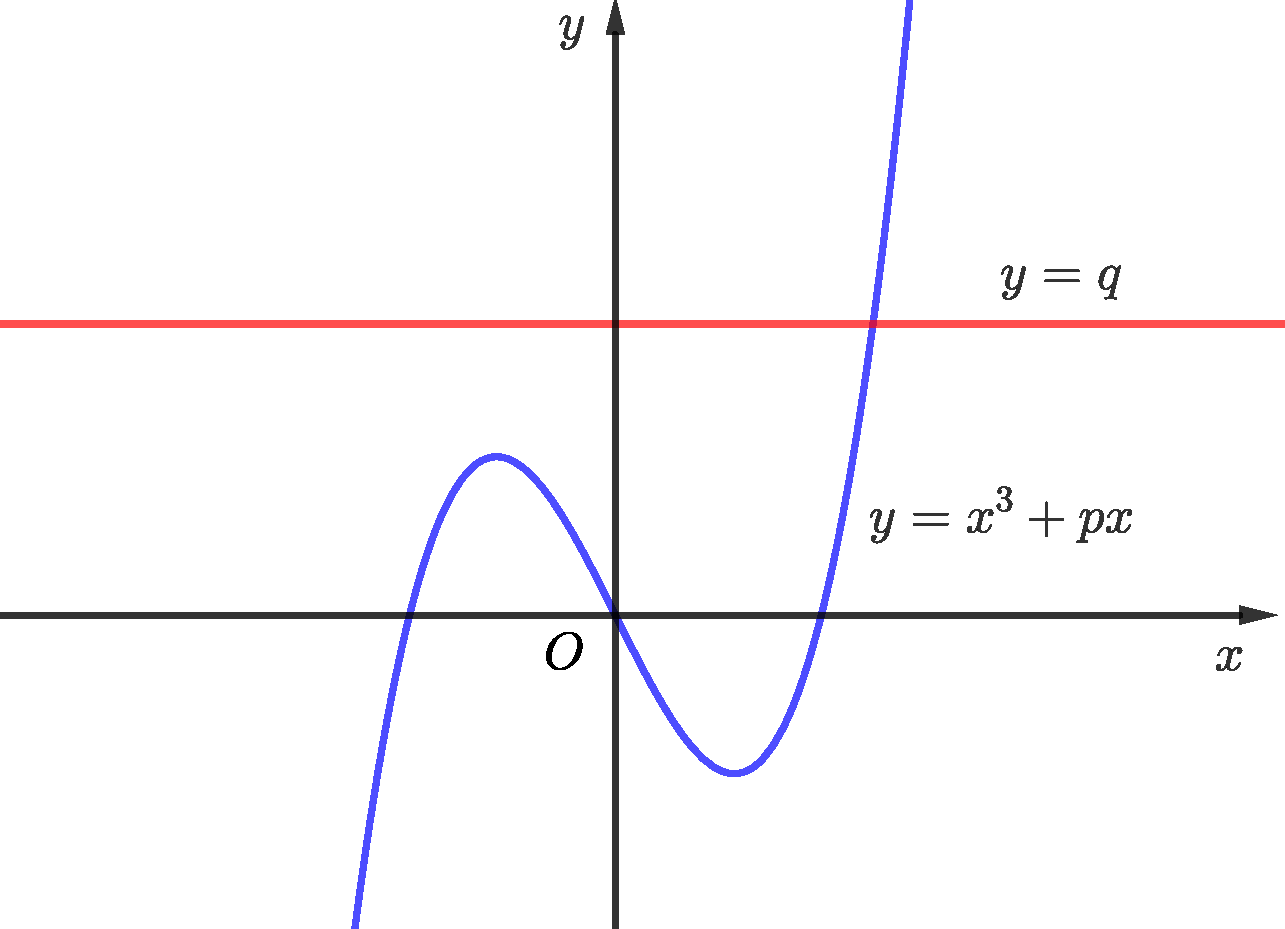
\includegraphics[width=0.8\textwidth]{grafici/cubica}
	\caption{L'equazione \ref{compl:iniziale} rappresentata graficamente tramite le funzioni $y=x^3+px$ e $y=q$.}
	\label{compl:cubica}
\end{figure}

\begin{proof}
	Partendo dalla \ref{compl:iniziale}, pongo $x=u+v$.
	\begin{align}
		(u+v)^3+p (u+v)            & = q \notag                  \\
		u^3+3u^2v+3uv^2+v^3+p(u+v) & = q \notag                  \\
		u^3+v^3+(3uv+p)(u+v)       & = q \label{compl:raddoppia}
	\end{align}
	La sostituzione $x = u + v$ non impone alcuna unicità, fissato il valore di $x$, delle due incognite sostitutive (l'equazione sostitutiva ha infinite soluzioni). Questo permette di scegliere una seconda relazione, per esempio che annulli il fattore $3uv + p$, che va a formare con la prima un sistema lineare in due equazioni in due incognite che, fissato $x$, ammette una e una sola soluzione (valori unici per $u$ e $v$):
	\begin{equation}
		\label{compl:sostsist}
		\begin{cases}
			x = u + v \\
			3uv + p = 0
		\end{cases}
	\end{equation}
	La relazione scelta permette di semplificare notevolmente l'equazione \ref{compl:raddoppia}, che si può ora esprimere tramite il sistema:
	\begin{subequations}
		\begin{numcases}{}
			3uv+p=0 \notag \\
			u^3+v^3=q \label{compl:u3v3}
		\end{numcases}
		\begin{numcases}{}
			v=-p/3u \notag \\
			u^3-\dfrac{p^3}{27u^3}=q \label{compl:quadratica-nascosta}
		\end{numcases}
	\end{subequations}
	Prendendo in considerazione l'equazione \ref{compl:quadratica-nascosta} e moltiplicando entrambi i membri\footnote{Risolvendo in $u$ il sistema \ref{compl:sostsist} si può notare che la variabile non è mai nulla, poiché supposto $p \neq 0$.} per $u^3$:
	\begin{align}
		u^3-\frac{p^3}{27u^3}-q     & = 0 \notag \\
		(u^3)^2-qu^3-\frac{p^3}{27} & = 0 \notag
	\end{align}
	Interpreto come un'equazione quadratica in $u^3$ e risolvo:
	\begin{gather}
		u^3=\frac{q\pm\sqrt{q^2+\dfrac{4p^3}{27}}}{2}= \notag \\ =\frac{q}{2}\pm\frac{1}{2}\sqrt{q^2+\frac{4p^3}{27}}= \notag \\
		=\frac{q}{2}\pm\sqrt{\frac{1}{4}\left(q^2+\frac{4p^3}{27}\right)}= \notag \\ =\frac{q}{2}\pm\sqrt{\left(\frac{q}{2}\right)^2+\left(\frac{p}{3}\right)^3}
	\end{gather}
	dove il radicando $\left(\frac{q}{2}\right)^2+\left(\frac{p}{3}\right)^3$ è detto discriminante ($\Delta$) dell'equazione iniziale (\ref{compl:iniziale}). Per $v^3$ si ottiene un risultato simmetrico, come si può dimostrare sfruttando l'uguaglianza \ref{compl:u3v3}:
	\[
		v^3 = q - u^3 = q - \left(\frac{q}{2} \pm \sqrt{\left(\frac{q}{2}\right)^2 + \left(\frac{p}{3}\right)^3}\right) = \frac{q}{2} \mp \sqrt{\left(\frac{q}{2}\right)^2 + \left(\frac{p}{3}\right)^3}
	\]
	In altre parole, quando si applica il più per $u$ si applica il meno per $v$ e viceversa. Tornando alla variabile $x=u+v$ risolvo l'equazione iniziale (scelgo un segno qualunque, pur mantenendo la coerenza tra i due, in quanto la somma è commutativa):
	\begin{equation}
		x = u + v = \sqrt[3]{\frac{q}{2} + \sqrt{\left(\frac{q}{2}\right)^2+\left(\frac{p}{3}\right)^3}}+\sqrt[3]{\frac{q}{2}-\sqrt{\left(\frac{q}{2}\right)^2+\left(\frac{p}{3}\right)^3}} \label{compl:risolutiva}
	\end{equation}
\end{proof}
\begin{examp}
	\begin{gather*}
		x^3 + 6x = 20 \\
		\Delta = \left( \frac{q}{2} \right)^2 + \left( \frac{p}{3} \right)^3 = \left( \frac{20}{2} \right)^2 + \left( \frac{6}{3} \right)^3 = 10^2 + 2^3 = 108 \\
		x = \sqrt[3]{10 + \sqrt{108}} + \sqrt[3]{10 - \sqrt{108}}
	\end{gather*}
	Ma
	\begin{align*}
		(1 \pm \sqrt3)^3 & =                                                                     \\
		                 & = 1^3 \pm 3 \cdot 1^2 \cdot \sqrt3 + 3 \cdot 1 \cdot (\pm \sqrt 3 )^2 \\
		                 & = 1 \pm 3 \sqrt 3 + 9 \pm 3 \sqrt 3                                   \\
		                 & = 10 \pm \sqrt{108}
	\end{align*}
	Quindi
	\[
		x=\sqrt[3]{10+\sqrt{108}}+\sqrt[3]{10-\sqrt{108}}=1+\sqrt3+1-\sqrt3=2
	\]
\end{examp}
La peculiarità della formula \ref{compl:risolutiva} è che permette di trovare la radice reale anche quando il discriminante è negativo. Infatti, applicando un ragionamento analogo a quello dell'esempio:
\begin{gather*}
	x^3 - 15x = 4 \\
	\Delta=\left(\frac{q}{2}\right)^2+\left(\frac{p}{3}\right)^3=\left(\frac{4}{2}\right)^2+\left(\frac{-15}{3}\right)^3=2^2+(-5)^3=-121 < 0 \\
	x=\sqrt[3]{2+\sqrt{-121}}+\sqrt[3]{2-\sqrt{-121}}
\end{gather*}
Il simbolo $\sqrt{-121}$ non ha significato. Tuttavia si può pensare di estendere la proprietà per cui $(\sqrt{a})^2=a$:
\begin{gather*}
	( 2 \pm \sqrt{-1} )^3 = 8 + 3*4( \pm \sqrt{-1} ) + 3*2( \pm \sqrt{-1} )^2 + ( \pm \sqrt{-1} )^3 = \\
	8 \pm 12\sqrt{-1} + 6(-1) + (-1)( \pm \sqrt{-1} ) = 2 \pm 11\sqrt{-1} = 2 \pm \sqrt{-121}
\end{gather*}
Quindi
\[
	x=\sqrt[3]{2+\sqrt{-121}}+\sqrt[3]{2-\sqrt{-121}}=2+\sqrt{-1}+2-\sqrt{-1}=4
\]
In questo modo senza comprendere il significato del simbolo $\sqrt{-1}$ possiamo ricavare la radice reale.

\section{Complessi}
Ragionamenti di questo tipo hanno portato alla creazione di un nuovo campo numerico: quello dei \textbf{complessi} (insieme $\C$).

\begin{defin}
	Si chiama insieme $\C$ dei numeri complessi l'insieme $\R^2$ (ovvero $\R\times\R$) e numero complesso ciascun elemento di $\C$, ossia una coppia ordinata di numeri reali.
\end{defin}
Per convenzione e semplicità il numero complesso $z$, che in quanto elemento di un prodotto cartesiano dovrebbe essere espresso con una coppia di coordinate nella forma $(a;b)$, si esprime invece nella forma
\[
	z = a + bi
\]
Il numero $a$ si chiama parte reale del numero complesso e si indica con $\re z$, il numero $b$ si chiama parte immaginaria del numero complesso e si indica con $\im z$. La parte reale e quella immaginaria si possono omettere quando rispettivamente $a$ e $b$ sono uguali a $0$.

\begin{defin}
	Due numeri complessi $z$ e $w$ si dicono:
	\begin{itemize}
		\item \emph{Uguali} se $\re z=\re w\land\im z=\im w$
		\item \emph{Coniugati} se $\re z=\re w\land\im z=-\im w$. Il coniugato di un numero $z$ si indica con $\bar z$
		\item \emph{Opposti} se $\re z=-\re w\land\im z=-\im w$
	\end{itemize}
	Inoltre si definisce modulo di un numero complesso $z$ e si indica con $\abs{z}$ il numero
	\[
		\sqrt{a^2+b^2}
	\]
\end{defin}


\subsection{Operazioni in \texorpdfstring{$\C$}{C}}
In $\C$ appare una proprietà del tutto nuova:
\[
	i^2=-1
\]
Presa in considerazione tale proprietà, in $\C$ si definiscono le seguenti operazioni, analoghe a ciò che avverrebbe nei reali considerando $a+bi$ un binomio nella variabile $i$:
\begin{defin}{Addizione di complessi}
	\[
		(a+bi)+(c+di)=(a+c)+(b+d)i
	\]
\end{defin}
\begin{defin}{Moltiplicazione di complessi}
	\begin{gather*}
		(a+bi)(c+di)=\\
		=ac+adi+bci+bdi^2=\\
		=ac+(ad+bc)i+bd(-1)=\\
		=(ac-bd)+(ad+bc)i
	\end{gather*}
\end{defin}

\subsubsection{Proprietà}
Nell'insieme $\C$ le operazioni godono di proprietà analoghe a quelle che valgono in $\R$.
\begin{description}
	\item[Addizione] L'addizione è commutativa e associativa, inoltre
		\begin{itemize}
			\item ha come elemento neutro il numero complesso $0+0i$ (o $0$)
			\item ogni numero complesso $a+bi$ ammette come opposto il numero $-a-bi$
		\end{itemize}
	\item[Moltiplicazione] La moltiplicazione è commutativa, associativa e distributiva rispetto all'addizione, inoltre
		\begin{itemize}
			\item ha come elemento neutro il numero complesso $1+0i$ (o $1$)
			\item ogni numero complesso $a+bi$, diverso da $0$, ammette come reciproco il numero $\dfrac{\bar z}{\abs{z}^2}=\dfrac{a-bi}{a^2+b^2}$, ossia il loro prodotto è uguale a $1$:
			      \begin{gather*}
				      ( a + bi ) \left( \frac{a - bi}{a^2 + b^2} \right) = \\
				      = \frac{a^2 - abi + abi + b^2}{a^2 + b^2} = \\
				      = \frac{a^2 + b^2}{a^2 + b^2} = 1
			      \end{gather*}
		\end{itemize}
\end{description}

\subsubsection{Proprietà del coniugio e del modulo}
L'operazione di coniugio, cioè di determinazione del coniugato di un numero complesso, e quella di modulo hanno alcune proprietà:
\begin{prop}
	Dati due numeri complessi $z=a+bi$ e $w=c+di$, valgono le seguenti proprietà:
	\begin{align}
		\label{compl:comouno}
		\bullet~ & \bar z=z\iff z\in\R                                  \\
		\label{compl:comodue}
		\bullet~ & \bar z=-z\iff z\in i\R                               \\
		\label{compl:comotre}
		\bullet~ & \overline{z+w}=\bar z+\bar w                         \\
		\label{compl:comoquattro}
		\bullet~ & \overline{z*w}=\bar z\bar w                          \\
		\label{compl:comocinque}
		\bullet~ & \abs{\bar z}=\abs{z}                                 \\
		\label{compl:comosei}
		\bullet~ & \abs{zw}=\abs{z}\abs{w}                              \\
		\label{compl:comosette}
		\bullet~ & \overline{\left(\frac{1}{z}\right)}=\frac{1}{\bar z} \\
		\label{compl:comootto}
		\bullet~ & z*\bar z=\abs{z}^2
	\end{align}
\end{prop}

% TODO: riformattare in un unico proof con un itemize/description con i ref ai vari punti
\begin{proof}[\ref{compl:comouno}]
	\begin{gather*}
		\bar z = z \iff \re \bar z = \re z \land \im \bar z = \im z \\
		a = a \quad \forall a \in \R \qquad b = -b \iff b = 0
	\end{gather*}
\end{proof}
\begin{proof}[\ref{compl:comodue}]
	Analogo alla precedente.
\end{proof}

\begin{proof}[\ref{compl:comotre}]
	\begin{equation*}
		\overline{z+w}=\overline{a+bi+c+di}=\overline{(a+c)+(b+d)i}=(a+c)-(b+d)i\\
	\end{equation*}
	\center al contempo:
	\begin{equation*}
		\bar z+\bar w= \overline{a+bi}+\overline{c+di}=a-bi+c-di=(a+c)-(b+d)i
	\end{equation*}
\end{proof}
\begin{proof}[\ref{compl:comoquattro}]
	\begin{equation*}
		\overline{z*w}=\overline{(a+bi)(c+di)}=\overline{(ac-bd)+(bc+ad)i}=(ac-bd)-(bc+ad)i\\
	\end{equation*}
	\center al contempo:
	\begin{equation*}
		\bar z*\bar w=\overline{a+bi}*\overline{c+di}=(a-bi)(c-di)=(ac-bd)-(bc+ad)i
	\end{equation*}
\end{proof}
\begin{proof}[\ref{compl:comocinque}]
	\begin{equation*}
		\abs{z} = \sqrt{a^2 + b^2} \\
	\end{equation*}
	\center al contempo:
	\begin{equation*}
		\abs{\bar z} = \sqrt{a^2 + ( -b )^2} = \sqrt{a^2 + b^2}
	\end{equation*}
\end{proof}
\begin{proof}[\ref{compl:comosei}]
	\begin{align*}
		\abs{zw} & = \sqrt{(ac-bd)^2+(bc+ad)^2} =                   \\
		         & = \sqrt{a^2c^2-2abcd+b^2d^2+b^2c^2+2abcd+a^2d^2} \\
	\end{align*}
	\center al contempo:
	\begin{align*}
		\abs{z}\abs{w} & = \sqrt{a^2+b^2}\sqrt{c^2+d^2}      \\
		               & =\sqrt{a^2c^2+a^2d^2+b^2c^2+b^2d^2}
	\end{align*}
\end{proof}
\begin{proof}[\ref{compl:comosette}]
	\begin{equation*}
		\overline{\left(\frac{1}{z}\right)}=\overline{\left(\frac{1}{a}+\frac{1}{b}i\right)}=\frac{1}{a}-\frac{1}{b}i\\
	\end{equation*}
	\center al contempo:
	\begin{equation*}
		\frac{1}{\bar z}=\frac{1}{\overline{a+bi}}=\frac{1}{a-bi}=\frac{1}{a}-\frac{1}{b}i
	\end{equation*}
\end{proof}
\begin{proof}[\ref{compl:comootto}]
	\begin{gather*}
		z*\bar z=(a+bi)(a-bi)=a^2-bi^2=a^2+b^2=\left(\sqrt{a^2+b^2}\right)^2=\abs{z}^2
	\end{gather*}
\end{proof}


\subsection{Rappresentazione grafica}
La definizione di numero complesso come coppia ordinata di numeri reali suggerisce una naturale rappresentazione geometrica dei numeri complessi nel piano cartesiano: il numero complesso $a+bi$ è rappresentato dal punto di coordinate $(a;b)$.\\
In questo contesto:
\begin{itemize}
	\item il piano viene chiamato \emph{piano di Argand-Gauss}
	\item l'asse $x$ viene chiamato \emph{asse reale}
	\item l'asse $y$ viene chiamato \emph{asse immaginario}
\end{itemize}

\subsubsection{Operazioni nel piano}
Se il numero complesso $z=a+bi$ può essere rappresentato nel piano di Argand-Gauss come un punto di coordinate $(a;b)$, può anche essere rappresentato con il vettore $\vec z$ di tali componenti. Questo permette di interpretare graficamente le operazioni di somma e differenza. Dati due numeri complessi $z$ e $w$:
\begin{itemize}
	\item il vettore che rappresenta $z+w$ è la somma dei vettori che rappresentano $z$ e $w$ (figura \vref{compl:fig1}).
	\item il vettore che rappresenta $z-w$ è la differenza dei vettori che rappresentano $z$ e $w$.
\end{itemize}

\begin{figure}[ht]
	\centering
	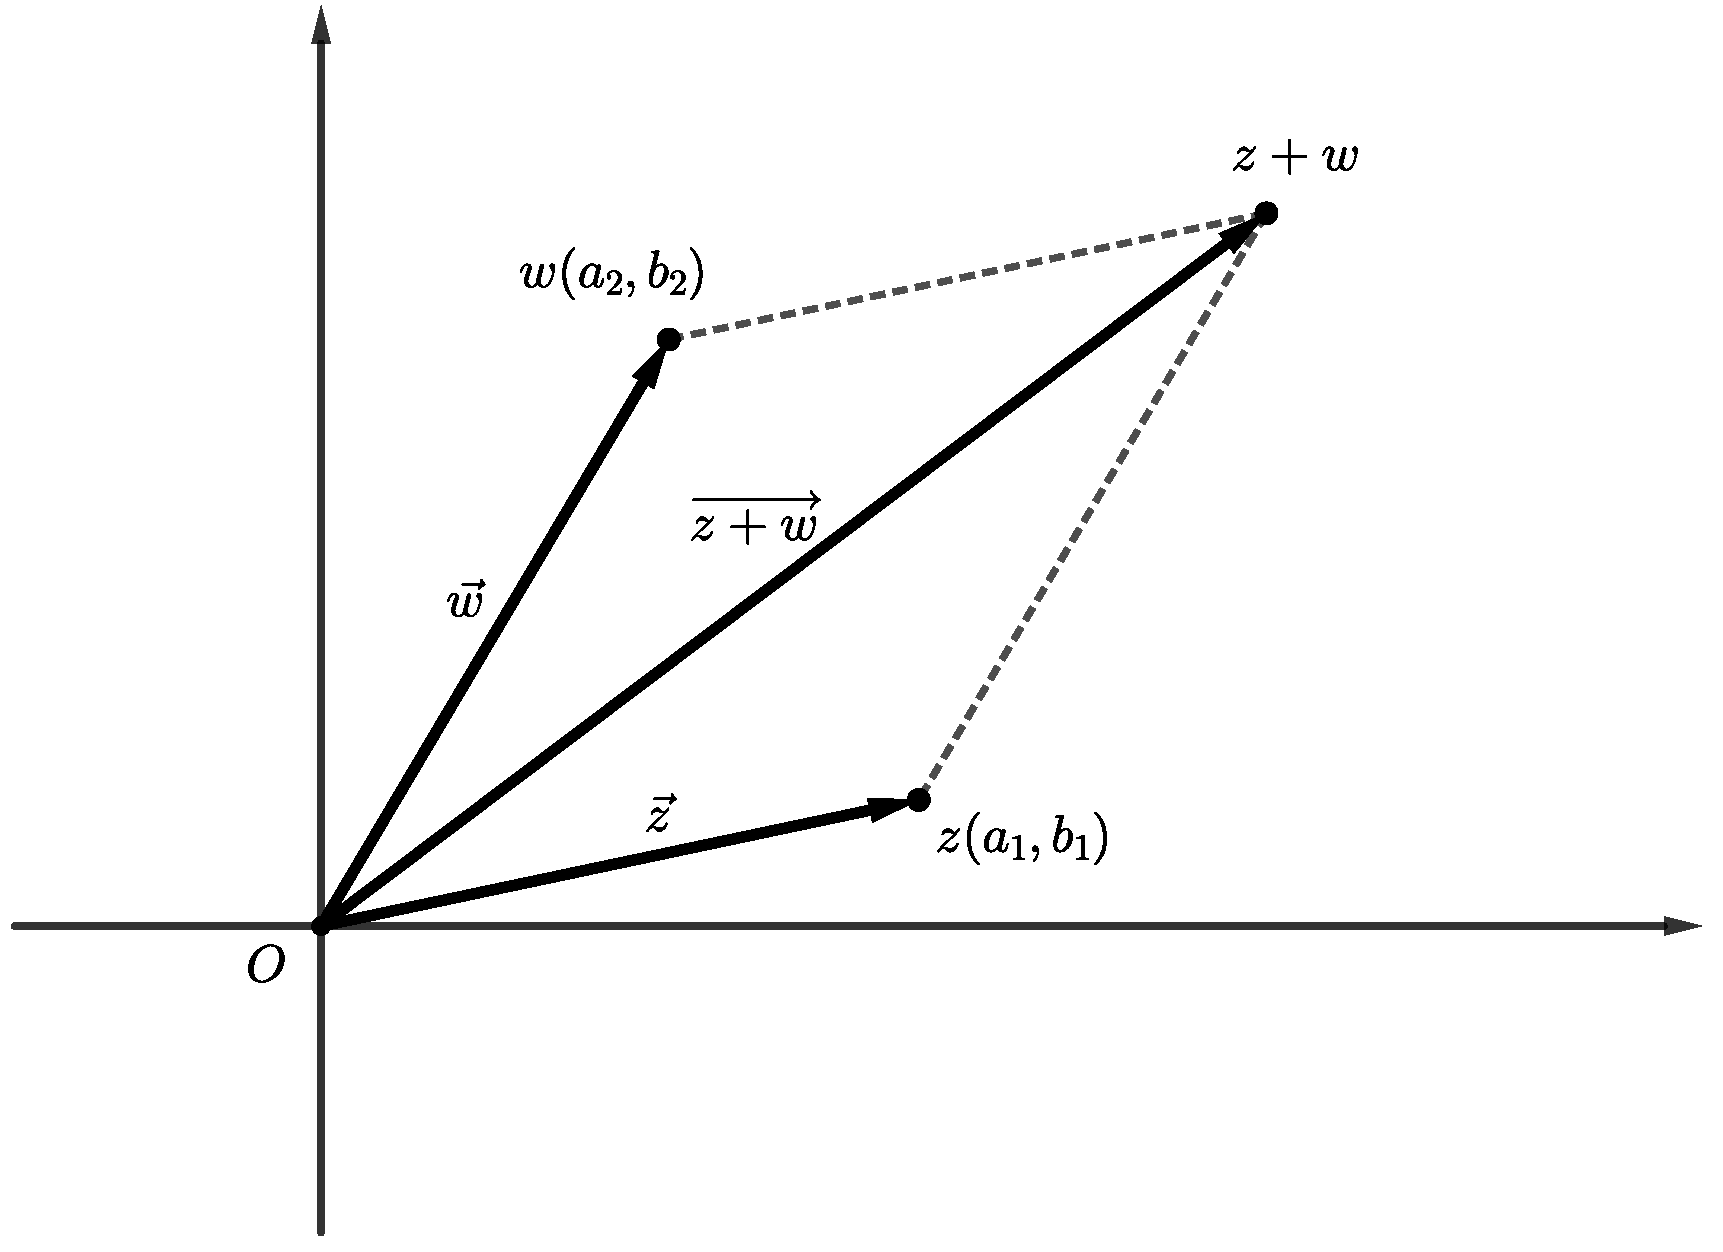
\includegraphics[width=0.7\textwidth]{grafici/complessi1}
	\caption{Due numeri complessi e la loro somma rappresentati nel piano di Argand-Gauss.}
	\label{compl:fig1}
\end{figure}


\subsection{Notazione trigonometrica}
I numeri complessi possono essere espressi in una forma, detta trigonometrica, la quale, pur essendo equivalente alla forma algebrica\footnote{Basti pensare che $\rho\cos\theta$ e $\rho\sin\theta$ sono le componenti del vettore $\vec z$}, possiede delle comode proprietà grafiche in riferimento al piano di Argand-Gauss:
\begin{equation}
	\label{compl:trigo}
	z=\rho(\cos\theta+i\sin{\theta})
\end{equation}
Dove $\rho$ indica il modulo $\abs{z}$ e $\theta$ l'argomento di $z$, ossia l'angolo che il vettore $\vec z$ forma con l'asse dei reali.

\begin{figure}[ht]
	\centering
	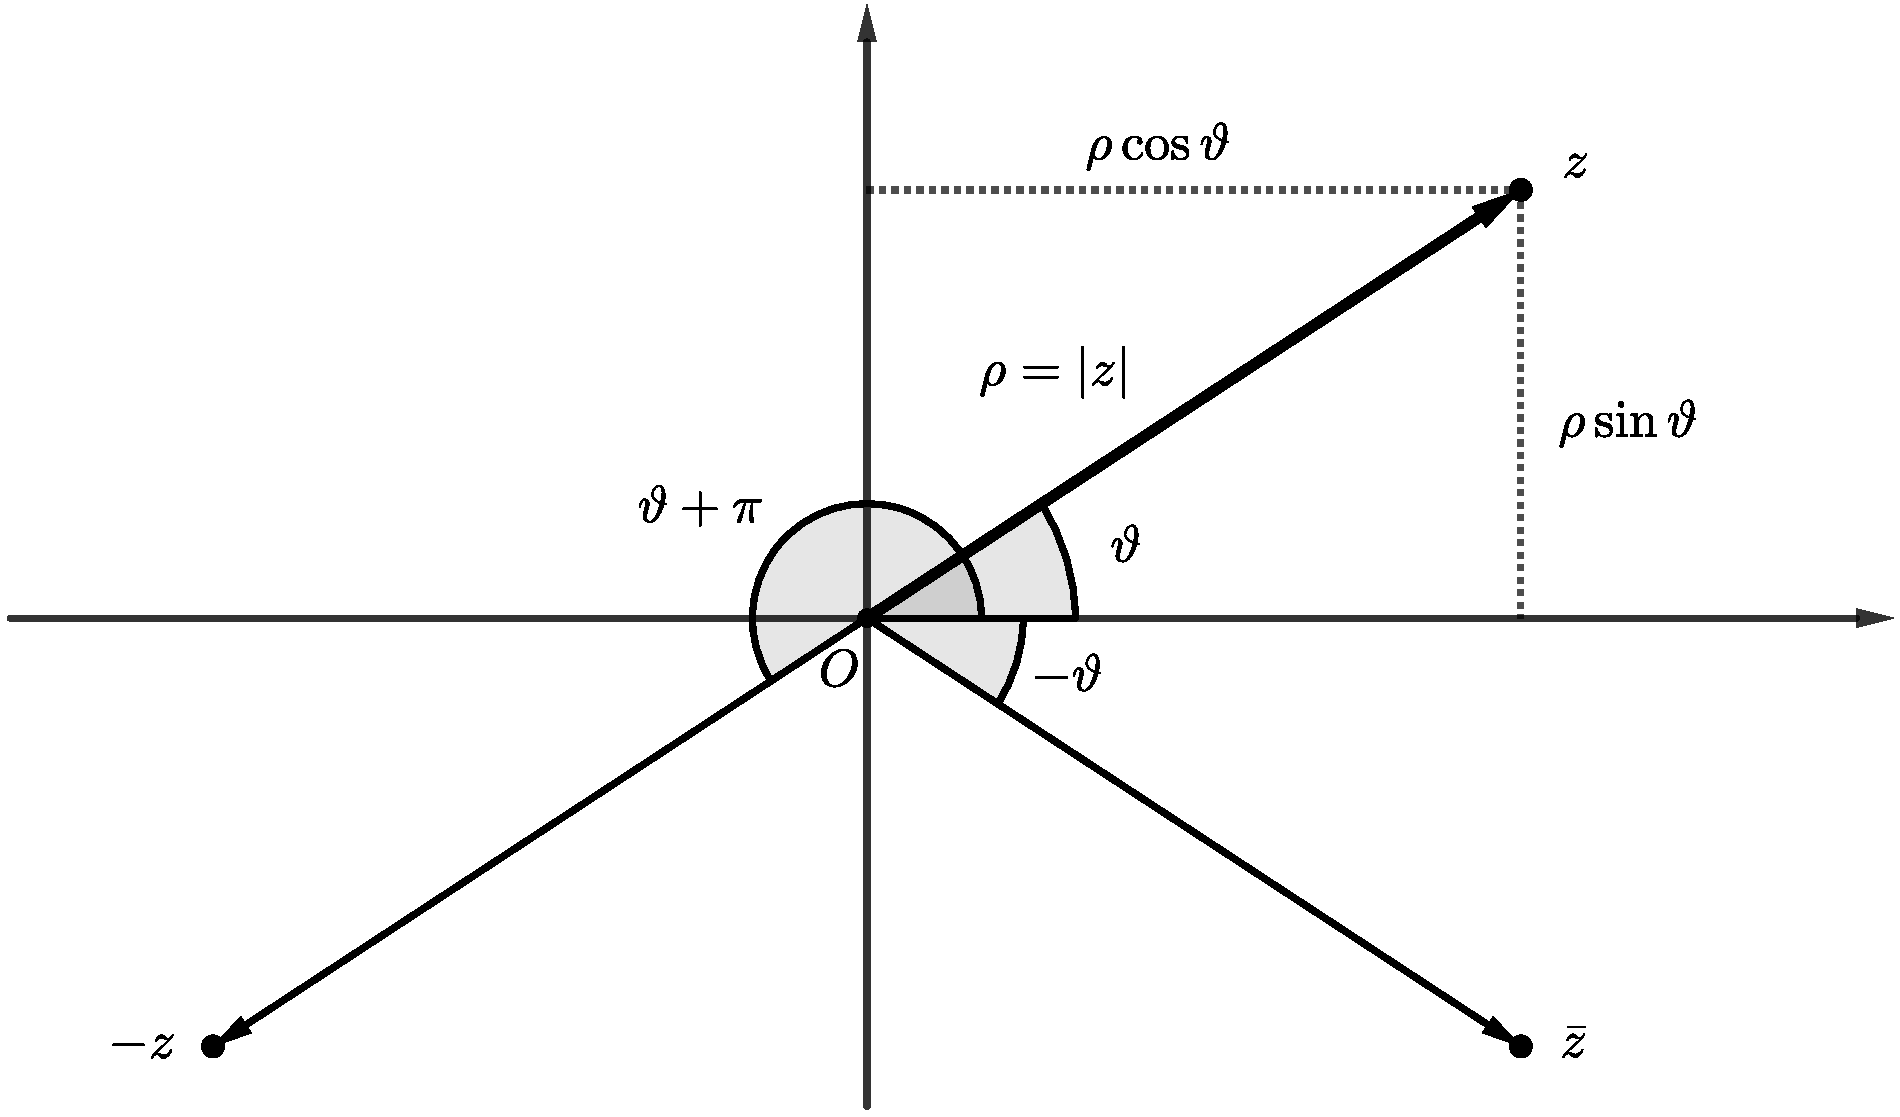
\includegraphics[width=0.9\textwidth]{grafici/complessi2b}
	\caption{Il numero complesso $z$, i suoi opposto e coniugato e i relativi parametri trigonometrici nel piano di Argand-Gauss}
	\label{compl:fig2}
\end{figure}

\subsubsection{Operazioni in forma trigonometrica}
In questo contesto due numeri complessi $z_1=\rho(\cos\theta+i\sin\theta)$ e $z_2=\sigma(\cos\varphi+i\sin\varphi)$ sono uguali se
\[
	\begin{cases}
		\rho=\sigma \\
		\theta=\varphi+2k\pi\qquad\text{con }k\in\Z
	\end{cases}
\]

Si possono facilmente esprimere alcune operazioni tra complessi in forma trigonometrica:
\begin{gather*}
	z_1\cdot z_2=\rho(\cos\theta+i\sin{\theta})\sigma(\cos\varphi+i\sin{\varphi})=\\
	\rho\sigma(\cos\theta\cos\varphi-\sin\theta\sin\varphi+i(\cos\theta\sin\varphi+\sin\theta\sin\varphi))=\\
	\rho\sigma(\cos(\theta+\varphi)+i\sin(\theta+\varphi))
\end{gather*}
Il prodotto di due numeri complessi in forma trigonometrica è un numero complesso che ha per modulo il prodotto dei moduli e per argomento la somma degli angoli. Geometricamente, avviene una dilatazione (o compressione) della distanza dall'origine e una rotazione rispetto agli assi. È facile dunque definire la potenza come moltiplicazione ripetuta:
\[
	z^n=\rho^n(\cos(n\theta)+i\sin(n\theta))
\]
E la potenza a esponente negativo come una potenza del reciproco:
\[
	z^{-n}=\frac{1}{\rho^{n}}(\cos(-n\theta)+i\sin(-n\theta))
\]

Alcuni numeri complessi notevoli in riferimento a $z$ così come espresso nella forma \ref{compl:trigo} (figura \vref{compl:fig2}):
\begin{align*}
	\bullet~ & -z=\rho(\cos(\theta+\pi)+i\sin(\theta+\pi))                                  \\
	\bullet~ & \bar z=\rho(\cos(-\theta)+i\sin(-\theta))                                    \\
	\bullet~ & z^{-1}=\frac{\bar z}{\abs{z}^2}=\frac{1}{\rho}(\cos(-\theta)+i\sin(-\theta))
\end{align*}


\section{Scomposizioni di polinomi a coefficienti reali}
Il teorema fondamentale dell'algebra, la quale dimostrazione non trattiamo, cita:
\begin{teor}[fondamentale dell'algebra]
	Ogni polinomio complesso (a coefficienti complessi) $P_n(z)$ di grado $n\geq1$ ammette radici complesse. In simboli:
	\begin{gather*}
		\forall P(z) \mid \text{\emph{grado}}(P(z))\geq1 \qquad \exists z_1\in\C \mid P(z)=(z-z_1)(P'(z))\\
		\text{con \emph{grado}} (P'(z))= \text{\emph{grado}} (P(z))-1
	\end{gather*}
\end{teor}
Poiché ogni $P'(z)$ ha anch'esso radici complesse, ogni polinomio ha $n$ radici e può essere espresso tramite prodotto di $n$ fattori di primo grado $(z-z_n)$

Per i polinomi a coefficienti reali vale inoltre un'altra proprietà:
\begin{teor}
	Se $P(z)$ è un polinomio a coefficienti reali, allora:
	\[
		\overline{P(z)}=P(\bar z)
	\]
\end{teor}
\begin{proof}
	\begin{gather*}
		\overline{P(z)}=\overline{a_0z^n+a_1z^{n-1}+\dots+a_{n-1}z+a_n}=\\
		=\overline{a_0z^n}+\overline{a_1z^{n-1}}+\dots+\overline{a_{n-1}z}+\bar a_n=\\
		=\bar a_0(\bar z)^n+\bar a_1(\bar z)^{n-1}+\dots+\bar a_{n-1}\bar z+\bar a_n=\\
		\text{essendo i coefficienti reali:}\\
		=a_0(\bar z)^n+a_1(\bar z)^{n-1}+\dots+a_{n-1}(\bar z)+a_n=P(\bar z)
	\end{gather*}
\end{proof}
\begin{corol}
	Le radici complesse di un polinomio a coefficienti reali vengono a coppie coniugate
\end{corol}
\begin{proof}
	\[
		P(z) = 0 \Rightarrow \overline{P(z)} = 0 \Rightarrow P(\bar z) = 0
	\]
	Per il teorema di Ruffini $z$ e $\bar z$ sono radici del polinomio.
\end{proof}
Si osserva che il prodotto di due fattori di primo grado derivanti da radici complesse coniugate è un polinomio di secondo grado a coefficienti reali:
\[
	(z-z_1)(z- \bar z_1)=z^2-(z_1+\bar z_1)z+\abs{z_1}^2
\]
Facendo dunque la scomposizione di un polinomio a coefficienti reali secondo il teorema fondamentale dell'algebra e moltiplicando a due a due i fattori a radici complesse coniugate, si ottiene una scomposizione in fattori di primo e secondo grado a coefficienti unicamente reali.

Inoltre osservando che la somma dei gradi dei fattori è uguale al grado del polinomio iniziale, si possono individuare due corollari relativi ai polinomi a coefficienti reali di grado pari e dispari:
\begin{corol}
	Ogni polinomio di grado dispari ha almeno una radice reale\footnote{È questa radice quella trovata per le cubiche depresse al paragrafo \ref{compl:cubidepresse}}
\end{corol}
\begin{corol}
	Ogni polinomio di grado pari ha radici reali in numero pari (zero incluso)
\end{corol}
Quanto al problema di determinare tali radici:
\begin{itemize}
	\item un'equazione di primo grado $ax+b=0$ ha un'unica soluzione: $z=-\dfrac{b}{a}$
	\item un'equazione di secondo grado $ax^2+bx+c=0$ ha due soluzioni:
	      \[
		      z_i=\frac{-b+d_i}{2a}
	      \]
	      dove $d_1$ e $d_2$ sono le due radici complesse di $\Delta=b^2-4ac$. Le soluzioni sono quindi reali se e solo se $\Delta\geq0$, altrimenti sono complesse coniugate.
\end{itemize}

\subsection{Scomposizioni in fratti semplici}
\label{frattisemplici}
Un'applicazione pratica della scomposizione dei polinomi a coefficienti reali è la scomposizione di un rapporto di polinomi in una somma di fratti semplici, cioè di rapporti del tipo $\frac{P(x)}{S(x)}$ in cui il grado del numeratore è minore del grado del denominatore e il denominatore è irriducibile in $\R$.

Dato un rapporto di polinomi $\frac{P(x)}{S(x)}$:
\begin{itemize}
	\item Se il grado di $P(x)$ è maggiore di quello di $S(x)$ si esegue la divisione, il quale risultato è in forma $Q(x)+R(x)$ (con $Q$ quoziente e $R$ resto) e si riscrive il rapporto iniziale nella forma
	      \[
		      \dfrac{P(x)}{S(x)}=\dfrac{Q(x)S(x)+R(x)}{S(x)}=Q(x)+\dfrac{R(x)}{S(x)}
	      \]
	      per poi ragionare su $\frac{R(x)}{S(x)}$ secondo il metodo seguente;
	\item Se il grado di $P(x)$ è minore di quello di $S(x)$ si riscrive il polinomio su un modello del tipo:
	      \begin{equation}
		      \label{compl:scomp}
		      \frac{P(x)}{S(x)}=\sum_k\sum_{m=1}^n \frac{A_m}{(x-a_k)^m}+\sum_j \frac{B_jx+C_j}{(x-z_j)(x-\bar z_j)}
	      \end{equation}
	      Dove $k$, e $j$ sono indici per le diverse radici e $n$ è la molteplicità di una radice di primo grado. Il prodotto dei due binomi con le radici complesse coniugate nella seconda sommatoria viene espresso in forma reale (cioè sviluppando il prodotto).
\end{itemize}
Per trovare A, B, C si applica poi il principio di identità dei polinomi:
\begin{enunc}[Principio di identità dei polinomi]
	Due polinomi sono identici se e solo se i coefficienti dei termini dello stesso grado sono uguali.
\end{enunc}
Quindi, si riduce l'intero polinomio sotto un unico minimo comune denominatore e ne si uguaglia la somma dei coefficienti delle $x$ all'n-esimo grado con il coefficiente dell'n-esimo grado di $x$ del polinomio originale. Mettendo a sistema le uguaglianze si ricavano i vari $A$, $B$ e $C$ e si riscrive il polinomio sostituendoli nella forma \ref{compl:scomp}.


\chapter{Reali, razionali e interi}
%% Copyright (C) 2019-2021 Alessandro Clerici Lorenzini
%
% This work may be distributed and/or modified under the
% conditions of the LaTeX Project Public License, either version 1.3
% of this license or (at your option) any later version.
% The latest version of this license is in
%   http://www.latex-project.org/lppl.txt
% and version 1.3 or later is part of all distributions of LaTeX
% version 2005/12/01 or later.
%
% This work has the LPPL maintenance status `maintained'.
%
% The Current Maintainer of this work is Alessandro Clerici Lorenzini
%
% This work consists of the files listed in work.txt


\section{Concetti di insiemistica}
In questa sezione si applicano a $\R$ e ai suoi sottoinsiemi concetti algebrici generalizzabili a un'ampia classe di insiemi.

\subsection{Maggioranti e minoranti}
\begin{defin}
	Posto $\emptyset\neq A\subset\R$ si dice insieme dei maggioranti di $A$ e si indica con $A^*$:
	\[
		A^*:=\{M\in\R\mid\forall a\in A\quad a\leq M\}
	\]
\end{defin}
% TODO: grafico retta reali
E, analogamente:
\begin{defin}
	Posto $\emptyset\neq A\subset\R$ si dice insieme dei minoranti di $A$ e si indica con $A_*$:
	\[
		A_*=:\{m\in\R\mid\forall a\in A\quad a\geq m\}
	\]
\end{defin}
Si osserva che $M\in A^*\land M'\geq M\Rightarrow M'\in A^*$ (se un numero $M'$ è maggiore o uguale a un maggiorante $M$ esso stesso è un maggiorante). Cosa analoga avviene per i minoranti. Ciò significa che i maggioranti e i minoranti sono descritti da intervalli illimitati, i primi del tipo $[M,+\infty)$ e i secondi del tipo $(-\infty,m]$.

Si ricorda che la negazione della proposizione che definisce i maggioranti (e allo stesso modo quella dei minoranti) è:
\begin{propo}
	\[
		M\notin A^*\iff\exists a\in A\mid a>M
	\]
\end{propo}


\subsection{Massimo e minimo}
\begin{defin}
	Si dice massimo di un insieme $\emptyset\neq A\subseteq\R$ e si indica con $\max A$:
	\[
		\max A=M\quad\Leftrightarrow\quad M\in A\land M\in A^*
	\]
\end{defin}
E, analogamente:
\begin{defin}
	Si dice minimo di un insieme $\emptyset\neq A\subseteq\R$ e si indica con $\min A$:
	\[
		\min A=m\quad\Leftrightarrow\quad m\in A\land m\in A_*
	\]
\end{defin}

Quando esiste, il massimo (così come il minimo) è unico:
\begin{proof}
	\begin{gather*}
		M,M'\in A^*\cap A\\
		\begin{cases}
			M\in A \\
			M'\in A^*
		\end{cases}\Rightarrow M\leq M'\\
		\begin{cases}
			M'\in A \\
			M\in A^*
		\end{cases}\Rightarrow M'\leq M
	\end{gather*}
	Ciò è possibile se e solo se $M=M'$
\end{proof}


\subsection{Estremi}
\begin{defin}
	Si dice estremo superiore di un insieme $\emptyset\neq A\subseteq\R$ e si indica con $\sup A$:
	\[
		\sup A:=
		\begin{cases}
			\min A^*\qquad & \text{se }A^*\neq\emptyset \\
			+\infty\qquad  & \text{se }A^*=\emptyset
		\end{cases}
	\]
\end{defin} E,
analogamente:
\begin{defin}
	Si dice estremo inferiore di un insieme $\emptyset\neq A\subseteq\R$ e si indica con $\inf A$:
	\[
		\inf A:=
		\begin{cases}
			\max A_*\qquad & \text{se  }A_*\neq\emptyset \\
			-\infty\qquad  & \text{se }A_*=\emptyset
		\end{cases}
	\]
\end{defin}
Si osservi che per dimostrare che un numero $S'$ non è un maggiorante è sufficiente:
\begin{gather*}
	\sup A=:S\\ S'<S\Rightarrow S'\notin A^*\\
	\text{ovvero, ponendo un $\varepsilon>0$ arbitrario:}\\
	S' = S-\varepsilon\notin A^*
\end{gather*}

Per gli insiemi definiti da un intervallo che non contiene l'estremo superiore, ossia insiemi del tipo $[a,b)$ oppure $(a,b)$, il massimo non esiste (mentre non esiste il minimo di insiemi definiti da intervalli che non contengono l'estremo inferiore):
\begin{proof}
	\begin{gather*}
		A=[a,b)\\
		b\notin A\Rightarrow b\neq M\\
		\text{pongo una variabile arbitraria } \varepsilon>0\\
		b-\varepsilon\notin A^*\Leftarrow b-\frac{\varepsilon}{2}>b-\varepsilon\land b-\frac{\varepsilon}{2}\in A
	\end{gather*}
	Il che vale per ogni valore possibile di $\varepsilon$ e quindi implica l'impossibilità dell'esistenza di un massimo.
\end{proof}
Analoga, ovviamente, è la dimostrazione nel caso del minimo.

%% Copyright (C) 2019-2021 Alessandro Clerici Lorenzini
%
% This work may be distributed and/or modified under the
% conditions of the LaTeX Project Public License, either version 1.3
% of this license or (at your option) any later version.
% The latest version of this license is in
%   http://www.latex-project.org/lppl.txt
% and version 1.3 or later is part of all distributions of LaTeX
% version 2005/12/01 or later.
%
% This work has the LPPL maintenance status `maintained'.
%
% The Current Maintainer of this work is Alessandro Clerici Lorenzini
%
% This work consists of the files listed in work.txt


\section{Fondamenti di logica}
Per implicazione si intende una proposizione, cioè un'affermazione di cui è possibile determinare il valore di verità, del tipo
\[
	A\Rightarrow B
\]
Dove $A$ e $B$ sono a loro volta proposizioni.
Per determinare il valore di verità dell'implicazione è necessario conoscere quello delle proposizioni che la compongono. Nella fattispecie:
\[
	\begin{array}{ccc}
		\toprule
		A & B & A\Rightarrow B \\
		\midrule
		V & V & V              \\
		V & F & F              \\
		F & V & V              \\
		F & F & V              \\
		\bottomrule
	\end{array}
\]
\subsubsection{Dimostrazione diretta}
Nella dimostrazione diretta, per dimostrare che la tesi $B$ è vera, si dimostra tramite un'implicazione logica $A\Rightarrow B$ valida (composta eventualmente da più passi) che l'ipotesi $A$ genera $B$ (eliminazione di implicazione). Ciò è possibile in quanto l'unico caso in cui l'ipotesi e l'implicazione sono vere è quello in cui la tesi è anch'essa vera.

\subsubsection{Dimostrazione contronominale}
Nella dimostrazione contronominale, vicina a quella per assurdo, si ottiene una tesi falsa tramite un'implicazione vera, il che significa come sancisce la tabella all'ultima riga che l'ipotesi è falsa.


\subsection{Il principio di induzione}
Il principio di induzione punta a dimostrare che una proposizione $P(n)$ sia vera per ogni $n$ maggiore o uguale a $k$. Esso si articola in due fasi:
\begin{description}
	\item[Base] dimostrare che $P(k)$ è verificata;
	\item[Passo] dimostrare a partire dall'ipotesi che $P(n)$ (dove $n$ è generico) sia verificata che lo sia anche $P(n+1)$ (implicazione $P(n)\Rightarrow P(n+1)$). Ogni passaggio deve valere per qualunque valore di $n\geq k$.
\end{description}
Questo come sancisce la tabella dimostra che anche $P(k+1)$ è verificata (tesi) e che quindi ripetendo il processo prendendo la tesi come ipotesi la proposizione è vera per ogni $n$ maggiore o uguale a $k$.

\begin{examp}
	Si intende dimostrare che la proposizione
	\[
		P(n): 0+1+\dots+n=\frac{n(n+1)}{2}
	\]
	è vera per ogni $n$ in $\N$.
	\begin{description}
		\item[Base] si dimostra che $P(0)$ è vera:
			\[
				0={0(0+1)}{2}
			\]
		\item[Passo] si dimostra che sapendo che $P(n)$ è vera anche $P(n+1)$ lo è:
			\begin{align*}
				0+1+\dots+n+n+1                 & =\frac{(n+1)[(n+1)+1]}{2}        \\
				\text{Poiché so che } 0+1       & +\dots+n=\frac{n(n+1)}{2}        \\
				\frac{n(n+1)}{2}+n+1            & =(n+1)\left(\frac{n+2}{2}\right) \\
				(n+1)\left(\frac{n}{2}+1\right) & =(n+1)\left(\frac{n}{2}+1\right)
			\end{align*}
	\end{description}
	La proposizione per il principio di induzione è quindi vera per ogni $n\in\N$.
\end{examp}
È fondamentale che nell'applicazione del secondo passo del principio di induzione non vengano applicate restrizioni all'insieme, come si può vedere dal seguente esempio:
\begin{examp}
	Si dimostra che se almeno una donna in un gruppo di $n$ donne è bionda, allora tutte le donne del gruppo sono bionde.
	\begin{description}
		\item[Base] in un gruppo di una donna c'è almeno una donna bionda, e tutte e $n=1$ le donne sono bionde ($(P(1)$ vera)
		\item[Passo] posto che la proposizione sia vera per $n$, è facile prendere da un gruppo di $n+1$ donne due gruppi distinti di $n$ donne che contengano la stessa donna bionda in modo che l'unione dei due contenga tutte le donne, e poiché la proposizione è vera per ipotesi per i gruppi di $n$ donne lo è anche per l'intero gruppo di $n+1$.
	\end{description}
	Questa dimostrazione concluderebbe che la proposizione è vera per ogni $n$, e che quindi le donne bionde sarebbero o tutte o nessuna. Chiaramente la proposizione non è vera: ci si pone dunque il problema di identificare l'errore.

	Esso avviene nel secondo passaggio. Il ragionamento applicato infatti si può utilizzare in tutti i casi tranne uno: quello di $n=1$. In questo caso, nell'insieme di $n+1=2$ donne è impossibile prendere due insiemi di una donna che abbiano tale donna in comune e la cui unione sia l'intero insieme. Poiché sono state applicate restrizioni al ragionamento, tutto il principio cade e la dimostrazione non è valida.
\end{examp}


\subsubsection{La disuguaglianza di Bernoulli}
\begin{teor}[Disuguaglianza di Bernoulli]
	\label{dis_berno}
	\[
		(1+x)^n\geq1+nx \qquad\forall x>-1,n\in\N
	\]
\end{teor}
\begin{proof}
	Per induzione su $n$:
	\begin{description}
		\item[Base]
			\[
				P(0): (1+x)^0\geq1+0x
			\]
			Ottengo $1\geq1$ che è vera.
		\item[Passo]
			\begin{gather}
				\label{eq:bernoB}
				P(n)\Rightarrow P(n+1): (1+x)^{n+1}\geq1+(n+1)x\\
				\text{riscrivo il primo membro}\notag\\
				(1+x)^{n+1}=(1+x)(1+x)^n\notag
			\end{gather}
			Ma $(1+x)^n>1+nx$ per ipotesi. Moltiplicando questa disuguaglianza per $(1+x)$ (cosa che posso fare in quanto la proposizione stessa impone la condizione $x>-1$) ottengo:
			\[
				(1+x)(1+x)^n\geq(1+x)(1+nx)
			\]
			Se quindi si dimostra che $(1+x)(1+nx)$, minore del primo membro della \ref{eq:bernoB}, è maggiore del suo secondo membro $1+(n+1)x$ (per ogni $n\in\N$), allora si dimostra l'implicazione:
			\[
				(1+x)(1+x)^n\geq(1+x)(1+nx)\geq1+(n+1)x
			\]
			Dimostrando:
			\begin{align*}
				(1+x)(1+nx) & \geq1+(n+1)x \\
				1+x+nx+nx^2 & \geq1+nx+x   \\
				nx^2        & \geq0
			\end{align*}
			L'ultima disequazione è sempre verificata per $n\in\N$, quindi l'implicazione è dimostrata.
	\end{description}
	L'ipotesi e l'implicazione sono vere per ogni $n\in\N$, quindi anche la tesi è dimostrata.
\end{proof}




\subsection{Proposizioni definitivamente vere}
\begin{defin}
	Si dice che una proposizione $P(n)$ con $n\in\N$ è definitivamente vera quando
	\[
		\exists\nu\in\N\mid P(n) \text{ è verificata }\forall n\geq\nu
	\]
	Mentre si dice che è definitivamente falsa quando è falsa per ogni $n$ maggiore o uguale a $\nu$
\end{defin}

Posta una proposizione definitivamente vera, è possibile fare alcune osservazioni:
\begin{lemma} \label{lem:defveresoglia}
	Se $P(n)$ è definitivamente vera per una soglia $\nu$ e $Q(n)=P(n+k)$, con $k\in\Z$, allora anche $Q(n)$ è definitivamente vera per $n>\nu-k$.
\end{lemma}
\begin{lemma}
	Poste due proposizioni definitivamente vere $P(n)$ per soglia $\nu_1$ e $Q(n)$ per $\nu_2$, la proposizione $P(n)\land Q(n)$ è definitamente vera per il maggiore dei $\nu$, il cui verifica contemporaneamente entrambe le proposizioni.
\end{lemma}


\subsubsection{La negazione}
È utile analizzare il significato della negazione di definitivamente vera:
\[
	\neg(\exists\nu\in\N\mid P(n) \text{ è verificata }\forall n\geq\nu)
\]
ossia
\[
	\forall\nu\in\N \quad\exists n\geq\nu\mid P(n) \text{ è falsa}
\]
Ciò significa che i valori di $n$ per cui $P(n)$ è falsa sono infiniti e arbitrariamente grandi.
\begin{examp}
	\[
		(-1)^n>0
	\]
	La proposizione non è né definitivamente vera né definitivamente falsa in quanto esistono valori di $n$ arbitrariamente grandi per cui essa è falsa, esattamente come valori arbitrariamente grandi per cui è vera. Comunque scelto un $\nu$, quindi, la proposizione sarà vera per alcuni valori di $n\geq\nu$ e falsa per altri.
\end{examp}


\chapter{Limiti di successioni}
%% Copyright (C) 2019-2021 Alessandro Clerici Lorenzini
%
% This work may be distributed and/or modified under the
% conditions of the LaTeX Project Public License, either version 1.3
% of this license or (at your option) any later version.
% The latest version of this license is in
%   http://www.latex-project.org/lppl.txt
% and version 1.3 or later is part of all distributions of LaTeX
% version 2005/12/01 or later.
%
% This work has the LPPL maintenance status `maintained'.
%
% The Current Maintainer of this work is Alessandro Clerici Lorenzini
%
% This work consists of the files listed in work.txt


\section{Successioni numeriche}
\begin{defin}
	Una successione è una funzione che ha come dominio l'insieme $\N$. Una successione nella variabile naturale $n$ viene indicata con $a_n$ (invece che con la notazione $a(n)$, più comune per le funzioni di dominio reale)
\end{defin}


\subsection{Progressioni}
\label{succ:progr}
Esempi notevoli di successioni sono le progressioni. Esse si dividono in
\begin{itemize}
	\item Progressioni aritmetiche come
	      \[
		      b_n=2n+3
	      \]
	      Nelle progressioni aritmetiche è costante la differenza tra valori consecutivi assunti dalla successione (cioè, per ogni $n$, $a_{n+1}-a_n$; nell'esempio $b_{n+1}=b_n+2$).
	\item Progressioni geometriche come
	      \[
		      c_n=3\cdot 2^n
	      \]
	      Nelle progressioni geometriche è invece costante il rapporto tra valori consecutivi della successione (nell'esempio $\frac{3\cdot2^{n+1}}{3\cdot2^n}=2$)
\end{itemize}
Nelle progressioni il valore che rimane costante tra successivi viene detto ragione della progressione.

\begin{prop}
	Per le progressioni aritmetiche vale:
	\begin{gather}
		b_{n+1}-b_n=d \\
		b_n=b_0+nd
	\end{gather}
\end{prop}
\begin{prop}
	Per le progressioni geometriche vale:
	\begin{gather}
		\frac{c_{n+1}}{c_n}=q \\
		c_n=c_0*q^n
	\end{gather}

\end{prop}
dimostrabili facilmente per induzione.


\subsection{Monotonia e limitatezza}

\subsubsection{Monotonia}
Due proprietà delle successioni sono fondamentali per il calcolo dei relativi limiti:
\begin{defin}[Monotonia]
	Una successione si dice monotòna crescente quando
	\[
		\forall n\in\N \qquad a_n\leq a_{n+1}
	\]
	E decrescente quando
	\[
		\forall n\in\N \qquad a_n\geq a_{n+1}
	\]
\end{defin}
\begin{examp}
	\[
		a_n=n^2-10n
	\]
	Mi chiedo se la successione è monotona crescente, cioè se
	\begin{align*}
		n^2-10n & \leq(n+1)^2-10n(n+1) \\
		n^2-10n & \leq n^2+2n+1-10n-10 \\
		2n-9    & \geq0
	\end{align*}
	La disuguaglianza non è vera per ogni $n$ naturale, ma solo per $n\geq\frac{9}{2}$. Ciò significa che la successione non è monotona crescente ma definitivamente crescente (cioè crescente a partire da un certo valore).
\end{examp}

\subsubsection{Limitatezza}
\begin{defin}[Limitatezza]
	Una successione si dice:
	\begin{itemize}
		\item \textbf{limitata superiormente} se esistono maggioranti della sua immagine:
		      \begin{gather*}
			      \{a_n\mid n\in\N\}^*\neq\emptyset\\
			      \text{Ovvero}\\
			      \exists M\in\R\mid a_n\leq M \qquad\forall n\in\N
		      \end{gather*}
		\item \textbf{limitata inferiormente} se esistono minoranti della sua immagine:
		      \[
			      \{a_n\mid n\in\N\}_*\neq\emptyset\\
		      \]
		\item \textbf{limitata} (o limitata bilateralmente) se esistono sia maggioranti sia minoranti della sua immagine:
		      \begin{gather*}
			      \{a_n\mid n\in\N\}^*\neq\emptyset \land \{a_n\mid n\in\N\}_*\neq\emptyset\\
			      \text{ovvero}\\
			      \exists R\in\R\mid \abs{a_n}\leq R \qquad\forall n\in\N
		      \end{gather*}
		      dove nella seconda espressione si utilizza $-R$ come minorante e $R$ come maggiorante.\footnote{Questa scelta non è limitante in quanto si sta scegliendo semplicemente uno dei minoranti (o maggioranti), e non l'estremo inferiore o superiore (ovvero si sceglie un $R$ che rispetti sia le condizioni per essere maggiorante che quelle cui il suo opposto sia minorante)}.
	\end{itemize}
\end{defin}
Una successione limitata è anche definitivamente limitata: se la condizione di limitatezza è verificata per ogni $n$ lo è anche per $n\geq k$. È vero però anche il contrario: una successione definitivamente limitata per $n\geq k$ con $a_n\leq R_1$ è anche limitata. È infatti sempre possibile determinare un valore $R_2$ che sia maggiore o uguale a $a_n$ per tutti i valori di $n$, in quanto i valori di $n$ minori di $k$ sono finiti (mentre per $n\geq k$ la condizione è verificata per ipotesi, a patto che $R_2\geq R_1$).
% TODO: aggiungere grafico

%% Copyright (C) 2019-2021 Alessandro Clerici Lorenzini
%
% This work may be distributed and/or modified under the
% conditions of the LaTeX Project Public License, either version 1.3
% of this license or (at your option) any later version.
% The latest version of this license is in
%   http://www.latex-project.org/lppl.txt
% and version 1.3 or later is part of all distributions of LaTeX
% version 2005/12/01 or later.
%
% This work has the LPPL maintenance status `maintained'.
%
% The Current Maintainer of this work is Alessandro Clerici Lorenzini
%
% This work consists of the files listed in work.txt


\section{Limiti}
Ci si potrebbe chiedere se al crescere di $n$ la successione si avvicini a un certo valore, finito o infinito. Lo studio di questo avvicinamento è lo studio del \textbf{limite} della successione.


\subsection{Limiti finiti}
Se una successione $a_n$, al crescere di $n$, si avvicina a un valore reale e finito $a$, si studia la distanza di $a_n$ da $a$, ovvero $\abs{a_n-a}$, in modo che sia minore di un errore arbitrario $\varepsilon>0$. Questa relazione deve valere definitivamente.
% TODO: limiti a valori $a^-$ e $a^+$
\begin{defin}[Limite finito di una successione]
	Il limite della successione $a_n$ è $a\in\R$ se e solo se
	\label{limsuc:defin}
	\[
		\forall\varepsilon>0\quad\exists\nu_\varepsilon\mid\abs{a_n-a}<\varepsilon\quad\forall n>\nu_\varepsilon
	\]
	In tal caso si scrive $a_n\to a$ (letto: $a_n$ tende ad $a$)
\end{defin}
% TODO: aggiungere grafico

\begin{examp}
	Dimostriamo che $\frac{1}{n}\to 0$:
	\begin{align*}
		(\frac{1}{n}-0) & <\varepsilon           \\
		n               & >\frac{1}{\varepsilon}
	\end{align*}
	Dove $\frac{1}{\varepsilon}$ è la soglia $\nu$ di cui alla definizione \ref{limsuc:defin}, che esiste per ogni valore scelto arbitrariamente di $\varepsilon$.
\end{examp}

\subsubsection{Restrizioni del dominio di $\varepsilon$}
Ci si può chiedere se l'arbitrarietà di $\varepsilon$ si può restringere a un sottoinsieme di $\R^+$.
\begin{itemize}
	\item dimostrando un limite per $\varepsilon>k$ (con $k\in\R^+$) si otterrebbe:
	      \[
		      \begin{cases}
			      \abs{a_n-a}<\varepsilon \\
			      \varepsilon>k
		      \end{cases}
	      \]
	      e non si avrebbe alcuna informazione per valori sufficientemente grandi di $n$ per cui $\abs{a_n-a}\leq k$.
	\item dimostrando un limite per $0<\varepsilon<k$ (con $k\in\R^+$), si dimostra che la disuguaglianza
	      \[
		      \abs{a_n-a}<\varepsilon<k
	      \]
	      è vera definitivamente. Ciò implica che $\abs{a_n-a}$ sia automaticamente minore definitivamente di ogni valore maggiore di k, per cui la dimostrazione è del tutto equivalente.
\end{itemize}

\subsubsection{Restrizioni del dominio di $n$}
Inoltre vale la seguente proprietà:
\begin{prop}
	\label{suc:trasl}
	\begin{equation}
		a_n\to a \quad\Rightarrow\quad a_{n+k}\to a
	\end{equation}
	Ossia
	\begin{equation*}
		\forall\varepsilon>0~\exists\nu_\varepsilon\mid\abs{a_n-a}<\varepsilon\quad\forall n>\nu_\varepsilon \Rightarrow \exists\nu'_\varepsilon\mid\abs{a_{n+k}-a}<\varepsilon\quad\forall n>\nu'_\varepsilon,\forall k\in\Z
	\end{equation*}
\end{prop}
% TODO dimostrazione
Ovvero: se $a_n$ tende ad $a$, significa che la distanza $\abs{a_n-a}$ è minore di un $\varepsilon>0$ arbitrario definitivamente, ciò significa che, a costo di una variazione della soglia, anche $a_{n+k}$ tende ad $a$, dal momento che si sta semplicemente ponendo un punto di partenza diverso per la successione (si veda anche il lemma \ref{lem:defveresoglia}).

In conclusione:
\begin{prop}
	\label{prop:epsn}
	Durante la dimostrazione di un limite si possono aggiungere condizioni, scegliendo di considerare $\varepsilon$ sufficientemente piccoli o $n$ sufficientemente grandi.
\end{prop}

\begin{examp}
	Cerco, se esiste, la soglia per cui $\frac{n+3}{2n-9}$ tende a $\frac{1}{2}$ definitivamente. In questo esempio viene sfruttata la proprietà \ref{prop:epsn} applicata a $n$:
	\begin{align*}
		\abs{\frac{n+3}{2n-9}-\frac{1}{2}} & <\varepsilon                         \\
		\abs{\frac{2n+6-2n+9}{2(2n-9)}}    & <\varepsilon                         \\
		\frac{15}{2\abs{2n-9}}             & <\varepsilon                         \\
		\abs{2n-9}                         & >\frac{15}{2\varepsilon}             \\
		\text{noto che } \abs{2n-9}        & = 2n-9 \text{ definitivamente}       \\
		2n-9                               & >\frac{15}{2\varepsilon}             \\
		n                                  & >\frac{15}{4\varepsilon}+\frac{9}{2}
	\end{align*}
\end{examp}
\begin{examp}
	Cerco, se esiste, la soglia per cui $\dfrac{1}{n-2\pi}\to 1$:
	\begin{align*}
		\abs{\frac{1}{n-2\pi}-1} & <\varepsilon                \\
		\frac{1}{n-2\pi}-1       & < 0\text{ definitivamente:} \\
		\frac{n-1-2\pi}{n-2\pi}  & <\varepsilon                \\
		n-1-2\pi                 & <\varepsilon(n-2\pi)        \\
		2\pi\varepsilon-1-2\pi   & <(\varepsilon-1)n
	\end{align*}
	Arrivati a questo punto, in cui il processo logico successivo sarebbe di dividere per $(\varepsilon-1)$ entrambi i membri, non si può porre $\varepsilon>1$, ma solo $\varepsilon<1$. Questo però ci porta a:
	\[
		n <\frac{2\pi\varepsilon-1-2\pi}{\varepsilon-1}
	\]
	Ovvero la disuguaglianza è definitivamente falsa, e in particolare non definitivamente vera. In questo caso il limite non è dimostrato.
\end{examp}


\subsection{Definizione generale}
Per il calcolo di limiti infiniti è necessario introdurre la definizione generale di limite di una successione, che certamente include anche il caso in cui il limite sia finito. È necessaria una definizione propedeutica:
\begin{defin}
	Viene definito intorno di un numero $a\in\R$ un insieme definito da un intervallo del tipo $(a-\varepsilon,a+\varepsilon)$ con $\varepsilon\in\R^+$. Si definisce intorno di $+\infty$ o $-\infty$ un intervallo del tipo $(M,+\infty)$ o $(-\infty,M)$ rispettivamente. L'insieme degli intorni di $a$ si indica generalmente con $I(a)$.
\end{defin}
\begin{defin}[Limite di una successione]
	Si definisce limite $l$ di una successione $a_n$, con $l\in\R^*$, un numero che gode della seguente proprietà:
	\[
		\forall U\in I(l)\quad a_n\in U\quad\text{definitivamente}
	\]
	Se il limite di una successione è finito si dice che essa converge, se esso è infinito si dice che essa diverge.
\end{defin}
\begin{examp}
	Dimostriamo che la successione $n^2-2n+5$ tende a $+\infty$:
	\begin{align*}
		n^2-2n+5         & >M     \\
		n^2-2n+5-M       & >0     \\
		\frac{\Delta}{4} & =1-5+M
	\end{align*}
	Per $M$ sufficientemente grandi, $\Delta>0$. Questo tipo di supposizioni su $M$ si possono fare perché si parla di intorni di $+\infty$, per cui diminuisce l'"ampiezza" dell'intorno. È un ragionamento analogo a quello espresso per $\varepsilon$ nella proprietà \ref{prop:epsn}, con la differenza che qui si possono scegliere solo $M$ più grandi. Ovviamente tutto il contrario vale per gli intorni di $-\infty$. La soluzione è quindi:
	\[
		n>1+\sqrt{M-4}\lor n<1-\sqrt{M-4}
	\]
	Mentre la seconda non è utile ai fini della dimostrazione, la prima fornisce una soglia per $n$ oltre la quale la successione appartiene all'intorno.
\end{examp}


\subsection{Proprietà}

\subsubsection{Unicità del limite}
\begin{prop}[Unicità del limite]
	Il limite di una successione, se esiste, è unico.
\end{prop}
\begin{proof}
	Si procede per assurdo, supponendo:
	\[
		a_n\to a\land a_n\to b \land a\neq b
	\]
	Se i numeri sono diversi, è possibile individuare due intorni degli stessi che non si intersechino:
	\begin{gather*}
		U\in I(a),V\in I(b)\\
		U\cap V=\emptyset
	\end{gather*}
	Per la definizione di limite, $a\in U$ definitivamente, e allo stesso tempo $a\in V$ definitivamente. Poiché la congiunzione di due proposizioni vere definitivamente è vera definitivamente, vale $a\in U\cap V$ definitivamente. Si è giunti a una contraddizione, per cui la tesi dev'essere vera. La dimostrazione si può estendere analogamente ai casi di limiti infiniti.
\end{proof}

\begin{prop}
	\[
		\begin{cases}
			a_n\to a \\
			a<b
		\end{cases}\Rightarrow a_n<b \text{ definitivamente}
	\]
\end{prop}
\begin{proof}
	Se per la definizione di limite comunque preso un intorno di $a$, $a_n$ appartiene all'intorno definitivamente, è sufficiente scegliere un intorno di $a$ che non includa $b$ per dimostrare che $b>a_n$ per ogni valore maggiore della soglia relativa a tale intorno.
\end{proof}

\begin{prop} \label{prop:permsegn}
	\[
		\begin{cases}
			a_n\to a \\
			a_n<b \text{ definitivamente}
		\end{cases}\Rightarrow a\leq b
	\]
\end{prop}
\begin{proof}
	Per assurdo, se $a$ fosse maggiore di $b$ si potrebbe scegliere un intorno di $a$ che non contiene $a_n$ definitivamente, in quanto $a_n<b$ definitivamente. Ciò ovviamente è in contraddizione con l'ipotesi che $a$ sia il limite della successione.
\end{proof}
Si noti che per $b=0$ la proprietà \ref{prop:permsegn} dimostra che una successione definitivamente negativa che ammette limite ha limite negativo, così come analogamente una successione definitivamente positiva che ammette limite ha limite positivo. Questo risultato è noto come \textbf{teorema di permanenza del segno}.

\begin{prop}
	\[
		\begin{cases}
			a_n\to a \\
			a\in\R
		\end{cases}\Rightarrow a_n \text{ è limitata}
	\]
\end{prop}
\begin{proof}
	Comunque scelto un intorno del limite, ognuno degli infiniti valori che $a_n$ assume oltre la soglia $\nu_\varepsilon$ è minore dell'estremo maggiore dell'intorno, mentre i valori esterni all'intorno sono finiti (essendo la successione definitivamente appartenente all'intorno) e si può quindi trovare un valore $M$ che sia maggiore di tutti.
\end{proof}
\begin{teor}[Piccolo teorema del confronto]
	\label{suc:confr1}
	\[
		\begin{cases}
			b_n\geq a_n \text{ definitivamente} \\
			a_n\to+\infty
		\end{cases}\Rightarrow b_n\to+\infty
	\]
\end{teor}
\begin{proof}
	Scelto arbitrariamente un $M$, vale per la definizione di limite la relazione $a_n>M$ definitivamente. Poiché $b_n>a_n$ definitivamente, oltre una certa soglia vale anche $b_n>M$, ovvero $b_n\to+\infty$. Lo stesso vale per relazioni d'ordine opposte che tendono a $-\infty$.
\end{proof}
\begin{teor}[Teorema del confronto]
	\label{teor:confronto}
	\[
		\begin{cases}
			a_n\leq b_n \leq c_n \text{ definitivamente} \\
			a_n\to l                                     \\
			c_n\to l
		\end{cases}\Rightarrow b_n\to l
	\]
\end{teor}
\begin{proof}
	Scelto un qualunque intorno di $l$, $a_n$ e $c_n$ vi appartengono definitivamente. Poiché $a_n\leq b_n \leq c_n$ definitivamente, esiste sicuramente una soglia oltre la quale $b_n$ appartiene all'intorno.
\end{proof}


\subsection{Casi notevoli}
Casi notevoli di limiti di successioni sono
\begin{itemize}
	\item
	      \begin{equation}
		      \frac{1}{n}\to 0^+
	      \end{equation}
	      La successione tende a $0^+$, cioè si avvicina a $0$ all'aumentare di $n$ mantenendo sempre valori positivi, ovvero $0\leq\frac{1}{n}<\varepsilon$. Se una successione si avvicina a $0$ dai valori negativi (per esempio $-\frac{1}{n}$) si dice che tende a $0^-$.
	\item
	      \begin{equation}
		      \frac{(-1)^n}{n}\to 0
	      \end{equation}
	      In questo caso la successione non tende né a $0^+$ né a $0^-$ in quanto l'avvicinamento della successione a $0$ assume sia valori positivi sia negativi qualunque sia l'ampiezza scelta dell'intorno.
	\item Il limite per la successione $(-1)^n$ non esiste, in quanto essa assume solo i valori $-1$ e $1$. Scegliendo un intorno di uno di questi due numeri in modo che escluda l'altro (così come un qualunque altro numero) è facile notare che il numero non può essere il limite.
	\item $n^\alpha$:
	      \begin{align}
		       & \to +\infty & \text{per }\alpha>0 \\
		       & \to 1       & \text{per }\alpha=0 \\
		       & \to 0^+     & \text{per }\alpha<0
	      \end{align}
	      \begin{itemize}
		      \item Nel primo caso $n^\alpha$ è crescente, per cui $n^\alpha>M$ con $M$ arbitrario, da cui la soglia $n>\sqrt[\alpha]{M}$;
		      \item nel secondo caso la successione è costante e uguale a $1$;
		      \item nel terzo caso $n^\alpha<\varepsilon$, cioè $n^{-\alpha} > \dfrac{1}{\varepsilon}$, da cui $n>\sqrt[-\alpha]{\dfrac{1}{\varepsilon}}$.
	      \end{itemize}
	\item $q^n$:
	      \begin{align}
		       & \to +\infty & \text{per }q>1       \label{eq:limnot3a} \\
		       & \to 1       & \text{per }q=1                           \\
		       & \to 0^+     & \text{per }0\leq q<1 \label{eq:limnot3c} \\
		       & \dots       & \text{per }q<0
	      \end{align}
	      \begin{itemize}
		      \item Nel primo caso $q^n>M$ si risolve in $n>\log_q M$;
		      \item nel secondo caso la successione è costante e uguale a $1$;
		      \item nel terzo caso $q^n<\varepsilon$ si risolve in $n>\log_q \varepsilon$;
		      \item per $q<0$, $q=-\abs{q}$, quindi $q^n=(-1)^n\abs{q}^n$. Il secondo fattore si riconduce al caso precedente, mentre il primo cambia costantemente valore tra $-1$ e $1$. Si deve dunque nuovamente distinguere tre casi:
		            \begin{itemize}
			            \item Per $\abs{q}>1$ il limite non esiste, in quanto per esponenti pari la successione si avvicina a $+\infty$, e per esponenti dispari a $-\infty$, per cui preso qualunque intorno di ciascuno dei due esso non conterrebbe i valori dell'altra parità di $n$;
			            \item per $\abs{q}=1$ il limite non esiste, in quanto la successione varia tra i valori $-1$ e $+1$ (vedi terzo caso notevole);
			            \item per $0<\abs{q}<1$ il limite è $0$, in quanto assume valori che cambiano costantemente segno e si avvicinano a $0$ analogamente caso (\ref{eq:limnot3c}), per la soglia $n>\log_{\abs{q}} \varepsilon$.
		            \end{itemize}
	      \end{itemize}
	\item $\log_\alpha n$:
	      \begin{align*}
		       & \to +\infty & \text{per }\alpha>1   \\
		       & \to -\infty & \text{per }0<\alpha<1
	      \end{align*}
	      \begin{itemize}
		      \item Nel primo caso la successione è monotona crescente e si trova la soglia $n>\alpha^M$;
		      \item nel secondo caso la successione è monotona decrescente e si trova la soglia $n>\alpha^M$.
	      \end{itemize}
	\item $n!$ e $n^n$ sono maggiori definitivamente di $n$, che tende a $+\infty$. Per il teorema \ref{suc:confr1} tendono quindi a $+\infty$.
\end{itemize}

\subsection{Algebra dei limiti}
\label{alglim}
Date due successioni $a_n\to a$ e $b_n\to b$, con $a,b\in\R$, si verificano le seguenti proprietà:
\begin{itemize}
	\item $a_n+b_n\to a+b$
	\item $a_n-b_n\to a-b$
	\item $a_n^{b_n}\to a^b$
	\item $\frac{a_n}{b_n}\to \frac{a}{b}$
\end{itemize}
Si dimostra la prima proprietà. Le dimostrazioni delle successive si basano su logica analoga.
\begin{proof}
	La tesi si traduce in:
	\begin{align*}
		\abs{(a_n+b_n)-(a+b)}                  & <\varepsilon \quad \forall\varepsilon>0 \\
		\text{ovvero}                                                                    \\
		\abs{(a_n-a)+(b_n-b)}                  & <\varepsilon                            \\
		\text{per disuguaglianza triangolare } & \text{sul primo membro:}                \\
		\abs{(a_n-a)+(b_n-b)}                  & < \abs{a_n-a}+\abs{b_n-b}
	\end{align*}
	I due addendi del secondo membro sono per ipotesi minori di qualunque errore positivo definitivamente, per esempio di $\frac{\varepsilon}{2}$. La loro somma è quindi minore di $\varepsilon$, comunque esso sia stato scelto:
	\[
		\abs{(a_n+b_n)-(a+b)}<\abs{a_n-a}+\abs{b_n-b}<\varepsilon
	\]
	Questo dimostra la tesi.
\end{proof}
Estendiamo la dimostrazione al caso in cui una delle due successioni, $b_n$, tende a $+\infty$. In questo caso la somma delle due tenderà anch'essa a $+\infty$.
\begin{proof}
	La disuguaglianza che bisogna provare è
	\[
		a_n+b_n>M
	\]
	Se $a_n$ converge, significa che è limitata, ovvero che $\abs{a_n}\leq R\quad\forall n$. Se $a_n>-R$, la disuguaglianza iniziale si riduce a:
	\begin{align*}
		-R+b_n & >M   \\
		b_n    & >M+R
	\end{align*}
	La disuguaglianza è verificata definitivamente in quanto $b_n\to+\infty$.
\end{proof}
Estendendo il problema a più di una successione divergente, si ottiene:
\begin{itemize}
	\item $+\infty+\infty=+\infty$
	\item $-\infty-\infty=-\infty$
\end{itemize}
Rimangono però operazioni che sembrano non poter essere svolte tra infiniti:
\begin{itemize}
	\item $+\infty-\infty$
	\item $\pm\infty*0$
	\item $\dfrac{0}{0}$
	\item $\dfrac{\infty}{\infty}$
	\item $\pm\infty^0$
	\item $0^0$
	\item $1^{\pm\infty}$
\end{itemize}
Questi sono detti casi di indecisione. I limiti di una successione composta da successioni che tendono ai valori di cui sopra non possono essere calcolati a prescindere, ma si ha bisogno di ulteriori informazioni sulla natura delle successioni.


\subsection{Numero di Nepero}
Si dimostra che l'interesse del $100\%$ di un capitale diviso in $n$ capitalizzazioni è uguale a
\[
	a_n=\left(n+\frac{1}{n}\right)^n
\]
Grazie alla disuguaglianza di Bernoulli (di cui al paragrafo \vref{dis_berno}) si dimostra che la successione è monotona crescente:
\begin{proof}
	Dire che la successione è crescente equivale a dire che, per $n\geq2$:
	\[
		\frac{a_n}{a_{n-1}}\geq1
	\]
	\begin{gather*}
		\frac{a_n}{a_{n-1}}=\frac{\left(n+\dfrac{1}{n}\right)^n}{\left(n+\dfrac{1}{n-1}\right)^{n-1}}=\frac{\left(\dfrac{n+1}{n}\right)^n}{\left(\dfrac{n}{n-1}\right)^{n-1}}=\\
		\left(\frac{n-1}{n}\right)^{n-1}\left(\frac{n+1}{n}\right)^n=\left(\frac{n}{n-1}\right)\left(\frac{n-1}{n}\right)^n\left(\frac{n+1}{n}\right)^n=\\
		\left(\frac{n}{n-1}\right)\left(\frac{n^2-1}{n^2}\right)^n=\left(\frac{n}{n-1}\right)\left(1-\frac{1}{n^2}\right)^n
	\end{gather*}
	Si nota che l'ultimo fattore rispetta i requisiti per applicare la disuguaglianza di Bernoulli:
	\begin{gather*}
		(1+x)^n\geq1+nx\qquad\forall n\geq0,x>-1\\
		-\frac{1}{n^2}>-1\qquad\forall n\geq2\\
	\end{gather*}
	Si può dunque applicare la disuguaglianza e moltiplicarla per il primo fattore, $\left(\dfrac{n}{n-1}\right)$, in quanto se ne conosce il segno, che è positivo:
	\[
		\left(\frac{n}{n-1}\right)\left(1-\frac{1}{n^2}\right)^n\geq\left(\frac{n}{n-1}\right)\left(1+n\left(-\frac{1}{n^2}\right)\right)
	\]
	Semplificando il secondo membro:
	\begin{gather*}
		\left(\frac{n}{n-1}\right)\left(1+n\left(-\frac{1}{n^2}\right)\right)=\frac{n}{n-1}-\left(\frac{n}{n-1}*\frac{n}{n^2}\right)=\\
		\frac{n}{n-1}-\frac{1}{n-1}=\frac{n-1}{n-1}=1
	\end{gather*}
	Quindi, in conclusione:
	\[
		\frac{a_n}{a_{n-1}}=\left(\frac{n}{n-1}\right)\left(1-\frac{1}{n^2}\right)^n\geq1
	\]
	La successione è monotona crescente.
\end{proof}
Tuttavia, calcolarne il limite non è immediato, in quanto si presenta nella forma di indecisione $1^{+\infty}$. Si introduce allora una seconda successione, questa volta strettamente decrescente:
\[
	b_n=\left(n+\frac{1}{n}\right)^{n+1}=\left(n+\frac{1}{n}\right)^n\cdot\left(n+\frac{1}{n}\right)
\]
Il primo fattore è uguale ad $a_n$, mentre il secondo è sempre maggiore di $1$. Si verifica quindi che $b_n>a_n$. Se le due successioni sono monotone in verso opposto e la seconda maggiore della prima, si deduce che non possono divergere. In particolare, è facile dimostrare l'esistenza di un maggiorante di $a_n$ (e analogamente di un minorante di $b_n$): $\forall n\in\N^+\exists b_1\in\R\mid a_n<b_n<b_1$, dove la prima disuguaglianza è vera per dimostrazione precedente e la seconda perché $b_n$ è strettamente decrescente. Viene naturale dedurre che $a_n$ tenda al minimo dei maggioranti, ovvero $a_n\to \sup\{a_n\}$.
\begin{teor}[Teorema di regolarità delle successioni monotone]
	\label{suc:rego}
	Se una successione $a_n$ è monotona crescente, ovvero $a_{n+1}\geq a_n \quad\forall n\in\N$, e $A=\{a_n\mid n\in\N\}$, allora $a_n\to \sup A$. Analogamente il limite di una successione monotona decrescente è uguale all'estremo inferiore dell'insieme delle sue immagini.
\end{teor}
\begin{proof} ~
	\begin{itemize}
		\item Se $A^*\neq\emptyset$ allora $l=\sup A\in\R$. Dimostrare che $l$ è il limite di $a_n$ significa dimostrare che la disuguaglianza
		      \[
			      \abs{a_n-l}<\varepsilon \qquad\forall\varepsilon>0
		      \]
		      è vera definitivamente. Dividendo la disequazione nelle due possibilità portate dal modulo:
		      \begin{itemize}
			      \item La disequazione
			            \begin{align*}
				            a_n-l & < \varepsilon   \\
				            a_n   & < l+\varepsilon
			            \end{align*}
			            è vera per ogni $n$ in quanto un numero maggiore di $l$ è senz'altro maggiorante di $A$;
			      \item quanto alla disequazione
			            \begin{equation*}
				            a_n-l>-\varepsilon
			            \end{equation*}
			            poiché $l$ è l'estremo superiore di $A$, esiste sicuramente un numero $l-\varepsilon$ che non sia un maggiorante, di cui quindi esiste almeno un valore di $a_n$ che sia maggiore:
			            \[
				            \exists\nu_\varepsilon\in\N\mid l-\varepsilon<a_{\nu_\varepsilon}
			            \]
			            Questo non dimostra il valore definitivo della verità della tesi, ma solo che esiste un valore $a_{\nu_\varepsilon}$ per cui la disuguaglianza è verificata. Introducendo l'ipotesi che $a_n$ sia monotona, tuttavia, vale
			            \[
				            n\geq\nu_\varepsilon\Rightarrow a_n>a_{\nu_\varepsilon}\qquad\forall n\in\N
			            \]
			            E poiché $a_{\nu_\varepsilon}>l-\varepsilon$, si verifica che $a_n>l-\varepsilon\quad\forall\varepsilon\in\R,\forall n\in\N$, ovvero che la tesi è vera definitivamente.
		      \end{itemize}
		\item Se $A^*=\emptyset$ bisogna dimostrare che $a_n\to\infty$, ovvero che la disuguaglianza
		      \[
			      a_n>M \qquad\forall M\in\R
		      \]
		      è vera definitivamente. poiché l'insieme dei maggioranti di $A$ è vuoto, $M$ non è un maggiorante. Procedendo come nella dimostrazione precedente per $l-\varepsilon$, si giunge alla conclusione che $a_n>M$ definitivamente.
	\end{itemize}
\end{proof}
Applicando il teorema alla successione di cui sopra si definisce il numero di Nepero $e$:
\[
	\left(1+\frac{1}{n}\right)^n\to e = 2.7182818\dots
\]
Siccome $a_n$ è strettamente crescente e $b_n$ strettamente decrescente, le due successioni consistono in approssimazioni rispettivamente per difetto e per eccesso di $e$ ($b_n$ tende a $e$ essendo equivalente al prodotto di $a_n$ per un fattore che tende a $1$). Per un'approssimazione più precisa, è utile stimare anche la distanza tra le due, che ovviamente tende a $0$:
\[
	b_n-a_n=\left(1+\frac{1}{n}\right)^n\left(\left(1+\frac{1}{n}\right)-1\right)
\]


\subsection{Soluzione dei casi di indecisione}
Ci si pone il problema di svolgere limiti di successioni composte da successioni che tendono a infinito nei modi dei casi di indecisione descritti al paragrafo \ref{alglim}. In alcuni casi avviene un'eliminazione puramente algebrica:
\[
	\frac{n^2}{n^3}=\frac{1}{n}\to0^+
\]
In altri casi è necessario individuare quale infinito ha un maggiore "impatto" sull'andamento della successione. I criteri della radice e del rapporto permettono, calcolando un limite ausiliario, di dedurre il limite della successione.
\begin{teor}[criteri della radice e del rapporto]
	\label{teor:sucradice}
	Data una successione $c_n$
	\[
		\begin{cases}
			c_n\geq0\quad\text{definitivamente} \\[1ex]
			\dfrac{c_{n+1}}{c_n}\to l\quad\lor\quad\sqrt[n]{c_n}\to l
		\end{cases}\Rightarrow
		\begin{cases}
			c_n\to0^+\quad     & \text{se }l<1 \\
			c_n\to+\infty\quad & \text{se }l>1
		\end{cases}
	\]
\end{teor}
\begin{proof}
	Si dimostra il teorema nel caso della radice $\sqrt[n]{c_n}$. Si noti che $l$ non può essere negativo in quanto la successione $c_n$ è positiva definitivamente (teorema di permanenza del segno).
	\begin{itemize}
		\item Se $0\leq l<+\infty$ allora per ogni intorno da $l-\varepsilon=p$ a $l+\varepsilon=q$ la successione $\sqrt[n]{c_n}$ vi cade definitivamente:
		      \[
			      p<\sqrt[n]{c_n}<q
		      \]
		      E quindi, definitivamente:
		      \[
			      p^n<c_n<q^n
		      \]
		\item Se $l=+\infty$ comunque scelto un valore $p$ positivo la successione ne è maggiore definitivamente:
		      \[
			      p<\sqrt[n]{c_n}
		      \]
		      Ovvero, definitivamente:
		      \[
			      p^n<c_n
		      \]
	\end{itemize}
	Si studia ora l'andamento delle successioni $p^n$ e $q^n$ al variare di $p$ e $q$.
	\begin{itemize}
		\item Se $q<1$ allora $q^n\to0^+$ (per la (\ref{eq:limnot3c})). Poiché per ipotesi $c_n\geq0$ si hanno tutte le ipotesi per applicare il teorema del confronto (\vref{teor:confronto}), considerando lo $0$ come una successione costante e tendente a $0$:
		      \[
			      \begin{cases}
				      0\leq c_n<q^n \\
				      q^n\to0^+
			      \end{cases}\Rightarrow c_n\to0^+
		      \]
		\item Se $p>1$ allora $p^n\to+\infty$ (per la (\ref{eq:limnot3a})). Si hanno tutte le ipotesi per applicare il teorema \vref{suc:confr1}:
		      \[
			      \begin{cases}
				      c_n>p^n \\
				      p^n\to+\infty
			      \end{cases}\Rightarrow c_n\to+\infty
		      \]
	\end{itemize}
	In tutti gli altri casi non si può concludere niente di utile alla dimostrazione. È sufficiente dunque scegliere $p$ e $q$ sufficientemente vicini al limite di $\sqrt[n]{c_n}$ (in particolare, $q<1$ se $l<1$ e $p>1$ se $l>1$) per dimostrare che a $l>1$ corrisponde $c_n\to+\infty$ e che a $l<1$ corrisponde $c_n\to0^+$. Si dimostra che lo stesso vale per il limite del rapporto; si può inoltre dimostrare che i due limiti $l$ sono uguali.
\end{proof}


\subsection{Limiti di successioni tipo}
Applichiamo ora il teorema per trovare i limiti di alcuni casi caratteristici:
\begin{itemize}
	\item
	      \[
		      c_n=\frac{n^\alpha}{q^n}\qquad\text{con }\alpha>0,q>1
	      \]
	      Sfruttando il criterio del rapporto:
	      \[
		      \frac{c_{n+1}}{c_n}=\frac{(n+1)^\alpha}{q^{n+1}}\cdot \frac{q^n}{n^\alpha}=\frac{q^n}{q\cdot q^n}\cdot \left(\frac{n+1}{n}\right)^\alpha=\frac{1}{q}\left(1+\frac{1}{n}\right)^\alpha
	      \]
	      Il secondo fattore tende a $1$, quindi il rapporto tende a $\frac{1}{q}$. Per ipotesi $q>1$, quindi il limite è minore di $1$. Per criterio del rapporto $c_n$ tende a $0^+$. Si noti che per $0<q\leq1$ il limite iniziale sarebbe stato immediato, da cui l'introduzione dell'ipotesi $q>1$.
	\item
	      \begin{gather*}
		      c_n=\frac{q^n}{n!}\qquad\text{con }q>1\\
		      \frac{c_{n+1}}{c_n}=\frac{q^{n+1}}{(n+1)!}\cdot \frac{n!}{q^n}=\frac{q}{n+1}\to0^+<1
	      \end{gather*}
	      Quindi $c_n\to0^+$.
	\item
	      \begin{gather*}
		      c_n=\frac{n!}{n^n}\\
		      \frac{c_{n+1}}{c_n}=\frac{(n+1)!}{(n+1)^{n+1}}\cdot \frac{n^n}{n!}=\frac{(n+1)n!}{(n+1)(n+1)^n}\cdot \frac{n^n}{n!}=\\
		      =\left(\frac{n}{n+1}\right)^n=\frac{1}{\left(1+\frac{1}{n}\right)^n}\to\frac{1}{e}<1
	      \end{gather*}
	      Quindi $c_n\to0^+$.
	\item
	      \[
		      c_n=\frac{\log_q n}{n^\alpha}\qquad\text{con }q>1
	      \]
	      Il metodo del rapporto ci porta a dimostrare che $\frac{c_{n+1}}{c_n}\to1$, unico caso in cui non si può dedurre niente sul limite di $c_n$. Per altre vie si può dimostrare che $c_n\to0^+$.
\end{itemize}


\chapter{Simboli di Landau}
%% Copyright (C) 2019-2021 Alessandro Clerici Lorenzini
%
% This work may be distributed and/or modified under the
% conditions of the LaTeX Project Public License, either version 1.3
% of this license or (at your option) any later version.
% The latest version of this license is in
%   http://www.latex-project.org/lppl.txt
% and version 1.3 or later is part of all distributions of LaTeX
% version 2005/12/01 or later.
%
% This work has the LPPL maintenance status `maintained'.
%
% The Current Maintainer of this work is Alessandro Clerici Lorenzini
%
% This work consists of the files listed in work.txt


% TODO: cosa succede se l'argomento dei simboli è 0?
Ai fini di semplificare e risolvere problemi nell'ambito dei limiti di successioni, è utile introdurre una nuova terminologia, sviluppata dal matematico tedesco Edmund Landau.

\section{\texorpdfstring{$o(\cdot)$ (o piccolo)}{o piccolo}}
Il primo simbolo è quello di $o(a_n)$ ($o$ piccolo di $a_n$), che viene definito come segue:
\begin{defin}
	\[
		o(b_n)=\left\{a_n \mid \frac{a_n}{b_n}\to0\right\}
	\]
	Inoltre, per notazione:
	\[
		a_n=o(b_n)\iff a_n\in o(b_n)
	\]
\end{defin}
Questo simbolo definisce una relazione, ma non un'uguaglianza. Questa relazione non gode infatti di due proprietà tipiche delle relazioni di equivalenza, la proprietà riflessiva e quella simmetrica (come si può dimostrare con semplici controesempi) mentre gode della proprietà transitiva:
\begin{prop}[Transitiva]
	\label{optrans}
	\[
		\forall a_n,b_n,c_n:
		\begin{cases}
			a_n=o(b_n) \\
			b_n=o(c_n)
		\end{cases}\Rightarrow a_n=o(c_n)
	\]
\end{prop}
\begin{proof}
	Per definizione, bisogna dimostrare che:
	\[
		\frac{a_n}{c_n}\to0
	\]
	Moltiplicando e dividendo per $b_n$:
	\[
		\frac{a_n}{b_n}\cdot \frac{b_n}{c_n}
	\]
	Per ipotesi entrambi i fattori tendono a $0$, quindi il limite del prodotto è $0$.
\end{proof}

\subsection{Proprietà e relazioni}
Un "uguaglianza" tra due $o$ non è riflessiva né simmetrica. In particolare:
\[
	o(a_n)=o(b_n)
\]
significa che ogni elemento dell'insieme $o(a_n)$ appartiene all'insieme $o(b_n)$, ovvero che l'insieme $o(a_n)$ è contenuto nell'insieme $o(b_n)$:
\[
	o(a_n)\subseteq o(b_n)
\]

\subsubsection{Somma di un $o$ e una successione}
Si introduce ora quello che si può considerare l'analogo per $o$ del primo principio di equivalenza delle equazioni.
\begin{teor}
	\[
		o(a_n)=b_n+o(c_n)\iff o(a_n)-b_n=o(c_n)
	\]
\end{teor}
\begin{proof}
	Si nota che il secondo membro (della prima proposizione) è la somma di un elemento con un insieme, cioè l'insieme delle somme di $b_n$ con ciascun elemento $\delta_n$ dell'insieme $o(c_n)$:
	\[
		b_n+o(c_n) = \{b_n+\delta_n\mid\delta_n\in o(c_n)\}
	\]
	Quindi la relazione iniziale si traduce nel dire che se un elemento $\gamma_n$ appartiene a $o(a_n)$, esso appartiene anche all'insieme dei $b_n+\delta_n$ (per quanto detto nel paragrafo precedente), ovvero esiste un $\delta_n$ in $o(c_n)$ tale che $\gamma_n=b_n+\delta_n$, dove l'ultimo $=$ ha il significato ordinario (non essendo applicato a $o$):
	\[
		\gamma_n=o(a_n)\Rightarrow\gamma_n=b_n+o(c_n)\Rightarrow\exists\delta_n=o(c_n)\mid\gamma_n=b_n+\delta_n
	\]
	E ciò vale per ogni $\gamma_n$ appartenente a $o(a_n)$. Essendo l'ultima un'equazione "classica" e quindi simmetrica, si può applicare:
	\[
		\delta_n=\gamma_n-b_n
	\]
	Quindi se $\delta_n$ appartiene a $o(c_n)$, significa che
	\[
		\gamma_n=o(a_n)\Rightarrow\gamma_n-b_n=o(c_n)
	\]
	In virtù del fatto che la relazione vale per ogni $\gamma_n$ che appartenga a $o(a_n)$, si può utilizzare $o(a_n)$ per indicare ogni elemento che vi appartiene:
	\[
		o(a_n)-b_n=o(c_n)
	\]
	% TODO: spiegare meglio
	Che tradotto usando la definizione significa anche
	\[
		\frac{\gamma_n}{a_n}\to0\Rightarrow\frac{\gamma_n-b_n}{c_n}\to0
	\]
	Analogo vale per l'implicazione inversa.
\end{proof}

\subsubsection{Prodotto di $o$ e una successione}
Esiste anche un analogo del secondo principio di equivalenza delle equazioni:
\[
	o(a_n)=b_n\cdot o(c_n)\iff\frac{o(a_n)}{b_n}=o(c_n)
\]


\subsection{Operazioni}

\subsubsection{Somma di $o(a_n)$ con se stesso}
\begin{teor}
	\[
		o(a_n)+o(a_n)=o(a_n)
	\]
\end{teor}
\begin{proof}
	Questa espressione equivale a dire, per la definizione, che la somma di due successioni $\gamma_{1_n}$ e $\gamma_{2_n}$ che divise per $a_n$ tendono a zero, a sua volta, se divisa per $a_n$, tende a zero. In simboli:
	\[
		\begin{cases}
			\dfrac{\gamma_{1_n}}{a_n}\to0 \\\\
			\dfrac{\gamma_{2_n}}{a_n}\to0 \\
		\end{cases}\Rightarrow\frac{\gamma_{1_n}+\gamma_{2_n}}{a_n}\to0\qquad\forall\gamma_{1_n},\gamma_{2_n}
	\]
	La dimostrazione è quasi immediata:
	\[
		\frac{\gamma_{1_n}+\gamma_{2_n}}{a_n}=\frac{\gamma_{1_n}}{a_n}+\frac{\gamma_{2_n}}{a_n}
	\]
	Poiché entrambi gli addendi tendono a $0$ per ipotesi, la somma tende a $0$, quindi $o(a_n)+o(a_n)=o(a_n)$.
\end{proof}

\subsubsection{Prodotto per una costante}
Come è facile dimostrare, i seguenti insiemi sono uguali:
\[
	o(c\cdot a_n)\qquad c\cdot o(a_n)\qquad o(a_n)
\]
\begin{proof}
	Si utilizza $o(a_n)$ per indicare ogni suo elemento.
	\begin{description}
		\item[$\bullet~ o(c\cdot a_n)=o(a_n)$] A partire dalla definizione:
			\[
				\frac{o(a_n)}{c\cdot a_n}\to 0\qquad\Rightarrow\qquad\frac{o(a_n)}{a_n}\cdot \frac{1}{c}\to0
			\]
			Nella seconda espressione, il secondo fattore è costante, quindi il primo tende a zero.
		\item[$\bullet~ c\cdot o(a_n) = o(a_n)$]
			\[
				c\cdot \frac{o(a_n)}{a_n}\to0
			\]
			Il primo fattore è una costante e il secondo tende a zero per definizione: il limite è zero.
		\item[$\bullet$] Per definizione, da $o(a_n)$:
			\[
				\frac{o(a_n)}{a_n}\to0
			\]
			Si può moltiplicare o dividere l'espressione per una costante, in quanto il limite rimane invariato. È possibile quindi svolgere un'operazione inversa rispetto alle due dimostrazioni precedenti e ottenere le espressioni che definiscono gli altri due insiemi.
	\end{description}
\end{proof}

\subsubsection{Differenza}
La differenza di due $o(a_n)$ non è altro che la somma del primo per il secondo moltiplicato per $-1$. Quindi, in virtù delle dimostrazioni precedenti:
\[
	o(a_n)-o(a_n)=o(a_n)+-1\cdot o(a_n)=o(a_n)+o(a_n)=o(a_n)
\]

\subsubsection{Prodotto per una successione}
I seguenti insiemi sono uguali:
\[
	b_n\cdot o(a_n)\qquad o(a_n\cdot b_n)
\]
pur non essendo uguali a $o(a_n)$.
\begin{proof} ~
	\begin{itemize}
		\item $b_n\cdot o(a_n)=o(a_n\cdot b_n)$:
		      \[
			      \frac{b_n\cdot o(a_n)}{a_n\cdot b_n}\to0\qquad\text{ovvero}\qquad\frac{o(a_n)}{a_n}
		      \]
		      Che tende a $0$ per definizione.
		\item $o(a_n\cdot b_n)=b_n\cdot o(a_n)$:
		      Utilizzando il "secondo principio":
		      \[
			      \frac{o(a_n\cdot b_n)}{b_n}=o(a_n)
		      \]
		      % TODO: ???
		      Ovvero, tradotto in limiti:
		      \[
			      \frac{o(a_n\cdot b_n)}{b_n\cdot a_n}\to0
		      \]
		      che è vero per definizione.
	\end{itemize}
\end{proof}

\subsubsection{$o(1)$ ($o$ piccolo di $1$)}
$o(1)$ è uno strumento che può tornare utile alla semplificazione di calcoli e nelle dimostrazioni. Infatti:
\begin{gather*}
	o(1)=\{a_n\mid a_n\to0\}\\
	o(a_n)\equiv o(a_n\cdot 1)\equiv a_n\cdot o(1)
\end{gather*}
Dove il simbolo $\equiv$ significa "equivale a"

Ecco un esempio di implementazione di questa proprietà:
\begin{examp}
	Stabilire per quali valori di $\alpha$ vale $o(n^\alpha)=o(n \ln n)$. Traducendo l'espressione tramite definizione:
	\[
		\frac{o(n^\alpha)}{n\ln n}\to0
	\]
	Traducendo in espressioni equivalenti:
	\[
		\frac{o(n^\alpha)}{n\ln n}\equiv\frac{n^\alpha}{n\ln n}\cdot o(1)\equiv\frac{n^{\alpha-1}}{\ln n}\cdot o(1)
	\]
	Per $\alpha>1$ il primo fattore tende a $+\infty$, producendo una forma di indecisione, mentre per $a\leq1$ il primo fattore tende a $0^+$, per cui moltiplicato per $o(1)$ tende a $0$.
\end{examp}

\subsubsection{$o(\cdot)$ composti}
Per la proprietà transitiva della relazione definita da $o$ (dimostrata come proprietà \vref{optrans}), vale la relazione:
\[
	o(o(a_n))=o(a_n)
\]

\section{\texorpdfstring{$\sim$ (asintotico)}{Asintotico}}
Il simbolo di asintotico viene così definito:
\begin{defin}
	\[
		a_n\sim b_n:\qquad\frac{a_n}{b_n}\to1
	\]
\end{defin}


\subsection{Proprietà}
La relazione gode di proprietà riflessiva (poiché $\frac{a_n}{a_n}=1$), simmetrica (poiché il reciproco di una successione che tende a 1 tende a 1) e transitiva:
\begin{proof}
	\begin{gather*}
		a_n\sim b_n\land b_n\sim c_n\Rightarrow a_n\sim c_n\\
		\frac{a_n}{c_n}=\frac{a_n}{b_n}*\frac{b_n}{c_n}\to1
	\end{gather*}
	In quanto i due fattori tendono a 1 per ipotesi.
\end{proof}
L'asintotico è quindi una relazione di equivalenza. Si dimostra che tutti gli elementi di una classe di equivalenza hanno lo stesso limite:
\begin{teor}
	\[
		\begin{cases}
			a_n\sim b_n \\
			b_n\to l
		\end{cases}\Rightarrow a_n\to l
	\]
\end{teor}
\begin{proof}
	\[
		a_n=\frac{a_n}{b_n}
	\]
	Che tende a $l$ in quanto il primo fattore tende a $1$ per definizione di asintotico e il secondo tende a $l$ per ipotesi.
\end{proof}


\subsection{Operazioni}
\begin{prop}
	\[
		\begin{cases}
			a_n\sim b_n \\
			A_n\sim B_n
		\end{cases}
		\begin{aligned}
			 & \Rightarrow\frac{a_n}{A_n}\sim\frac{b_n}{B_n}             \\
			 & \Rightarrow a_n\cdot A_n\sim b_n\cdot B_n                 \\
			 & \Rightarrow a_n^\alpha\sim b_n^\alpha\quad\forall\alpha>0
		\end{aligned}
	\]
\end{prop}
\begin{proof}
	Si dimostra la prima implicazione, in quanto le altre ne seguono direttamente. Traducendo la tesi in simboli:
	\[
		\frac{a_n/A_n}{b_n/B_n}\to1
	\]
	Semplificando l'espressione:
	\[
		\frac{a_n}{b_n}\cdot \frac{B_n}{A_n}
	\]
	Che tende a $1$ in quanto prodotto di due successioni tendenti a $1$ per ipotesi.
\end{proof}
Somme ed esponenziali non godono delle stesse proprietà, mentre per i logaritmi si pone un'ulteriore condizione:
% TODO: aggiungere controesempio per necessaria seconda condizione: n/(n+1) e (n+1)/n
\begin{prop}
	\[
		\begin{cases}
			a_n\sim b_n   \\
			b_n\to+\infty \\
			0<q\neq1
		\end{cases}\Rightarrow\log_qa_n\sim\log_qb_n
	\]
\end{prop}
\begin{proof}
	\[
		\frac{\log_qa_n}{\log_qb_n}=\frac{\log_q\left(\dfrac{a_n}{b_n}\cdot b_n\right)}{\log_qb_n}=\frac{\log_q(a_n/b_n)+\log_qb_n}{\log_qb_n}=\frac{\log_q(a_n/b_n)}{\log_qb_n}+1
	\]
	L'ultima espressione è la somma di un addendo che tende a $0$ e $1$, quindi il limite è $1$.
\end{proof}

La seguente è una proprietà dell'asintotico, utile in particolare in alcune dimostrazioni, che gli permette di essere scambiato con l'$o$ piccolo:
\begin{prop}
	\[
		a_n\sim b_n\iff a_n=b_n+o(b_n)
	\]
\end{prop}
\begin{proof}
	\begin{gather*}
		\frac{a_n}{b_n}\to1\\
		\text{quindi}\\
		\frac{a_n}{b_n}-1\to0\\
		\frac{a_n-b_n}{b_n}\to0\\
		\text{ergo}\\
		a_n-b_n=o(b_n)\\
		a_n=b_n+o(b_n)
	\end{gather*}
\end{proof}
\begin{examp}
	\begin{gather*}
		n^2+n\log n+\frac{n^6}{2^n}=\\
		n^2+o(n^2)+o(1)=n^2+o(n^2)+o(n^2)=n^2+o(n^2)\sim n^2\to+\infty
	\end{gather*}
\end{examp}

\begin{teor}
	\[
		a_n\sim b_n\Rightarrow o(a_n)\equiv o(b_n)
	\]
\end{teor}
\begin{proof}
	Si dimostra solo l'implicazione $o(a_n)=o(b_n)$. Poiché l'ipotesi è simmetrica, anche la tesi lo sarà. Traducendo la tesi secondo la definizione:
	\[
		\frac{o(a_n)}{b_n}=\frac{a_n\cdot o(1)}{b_n}=\frac{a_n}{b_n}\cdot o(1)
	\]
	Che tende a $0$ in quanto prodotto di un fattore che tende a $1$ (per ipotesi) e uno che tende a $0$ (per definizione).
\end{proof}

\section{\texorpdfstring{$O$, $\Omega$ e $\Theta$}{O, Omega e Theta} grandi}
I cosiddetti simboli grandi di Landau vengono definiti non più con un limite, ma con un intervallo limitante, nei modi che seguono:
\begin{defin}
	\begin{align*}
		\bullet~ & a_n=O(b_n):\quad\exists:                &       & \abs{\frac{a_n}{b_n}}\leq C\quad & \text{definitivamente} \\
		\bullet~ & a_n=\Omega(b_n):\quad\exists c>0:       &       & \abs{\frac{a_n}{b_n}}\geq c\quad & \text{definitivamente} \\
		\bullet~ & a_n=\Theta(b_n):\quad\exists 0<c\leq C: & c\leq & \abs{\frac{a_n}{b_n}}\leq C\quad & \text{definitivamente}
	\end{align*}
\end{defin}

\subsection{Proprietà}
Come è immediato dimostrare, poiché una successione è asintotica a se stessa, tutte le precedenti relazioni godono della proprietà riflessiva. Diverso è per la proprietà simmetrica:
\begin{gather*}
	a_n=O(b_n)\overset{?}{\Rightarrow} b_n=O(a_n)\\
	\exists C<+\infty: \abs{\frac{a_n}{b_n}}\leq C\quad\text{definitivamente}\\
	\text{ovvero}\\
	\exists C<+\infty: \abs{\frac{b_n}{a_n}}\geq \frac{1}{C}\quad\text{definitivamente}
\end{gather*}
L'ultima proposizione corrisponde con la definizione di $b_n=\Omega(a_n)$ (dove $1/C>0$ poiché $C\in\R$), infatti:
\[
	a_n=O(a_n)\iff b_n=\Omega(a_n)
\]
Lo stesso vale per $\Omega$, mentre per $\Theta$:
\begin{gather*}
	a_n=\Theta(a_n)\iff b_n=\Theta(a_n)\\
	\exists 0<c\leq C<+\infty: c\leq\abs{\frac{a_n}{b_n}}\leq C\quad\text{definitivamente}\\
	\text{ovvero}
	\exists 0<c\leq C<+\infty: \frac{1}{c}\geq\abs{\frac{b_n}{a_n}}\geq\frac{1}{C}\quad\text{definitivamente}
\end{gather*}
Che rispetta ancora la definizione di $a_n=\Theta(b_n)$.

La proprietà transitiva è invece propria di tutti i simboli grandi di Landau:
\begin{prop}
	\[
		\begin{cases}
			a_n=\Omega(b_n) \\
			b_n=\Omega(c_n)
		\end{cases}\Rightarrow a_n=\Omega(c_n)
	\]
\end{prop}
\begin{proof}
	\begin{gather*}
		\exists c>0: \abs{\frac{a_n}{b_n}}\geq c\quad\text{definitivamente}\\
		\abs{\frac{a_n}{b_n}}=\abs{\frac{a_n}{b_n}}\abs{\frac{b_n}{c_n}}
	\end{gather*}
	Il primo fattore è maggiore definitivamente di un valore $c_1$ per ipotesi, e il secondo di un valore $c_2$. Il loro prodotto sarà quindi maggiore del valore $c_1*c_2$ definitivamente, il che significa che $a_n=\Omega(c_n)$.
\end{proof}
\begin{examp}
	\[
		n^2+n\overset{?}{=}O(n^2)
	\]
	Per dimostrare la relazione, bisogna trovare un $C<+\infty$ per cui la seguente disuguaglianza è verificata definitivamente:
	\begin{align*}
		\abs{\frac{n^2+n}{n^2}} & \leq C   \\
		\frac{n^2+n}{n^2}       & \leq C   \\
		1+\frac{1}{n}           & \leq C   \\
		\frac{1}{n}             & \leq C-1
	\end{align*}
	Poiché $1/n$ è sempre minore o uguale a $1$, è sufficiente l'esempio $C=2$ per dimostrare che esiste un $C$ consono alla definizione:
	\[
		\frac{1}{n}\leq 2-1
	\]
	Quanto al problema di determinare tutte le possibili $C$, si riscrive la disequazione nel seguente modo:
	\[
		1\leq(C-1)n
	\]
	La quale si comporta diversamente a seconda del valore di $C$:
	\begin{align*}
		\bullet~ & C>1:\quad & n & \geq\frac{1}{C-1}\quad & \text{definitivamente vera}  \\
		\bullet~ & C=1:\quad & 1 & \leq0\quad             & \text{falsa}                 \\
		\bullet~ & C<1:\quad & n & \leq\frac{1}{C-1}\quad & \text{definitivamente falsa}
	\end{align*}
	Quindi il primo caso è l'unico in cui la condizione è verificata.
\end{examp}

Un teorema molto utile nel caso in cui il rapporto di due successioni tenda a un limite (ma che non dice niente in caso contrario) è il seguente:
\begin{teor}
	Posto:
	\[
		\abs{\frac{a_n}{b_n}}\to L
	\]
	Allora:
	\begin{align*}
		\bullet~ a_n=O(b_n)      & \iff L<+\infty   & \text{con }C\geq L \\
		\bullet~ a_n=\Omega(b_n) & \iff L>0         & \text{con }c\leq L \\
		\bullet~ a_n=\Theta(b_n) & \iff 0<L<+\infty &
	\end{align*}
\end{teor}
\begin{proof}
	Si dimostra il teorema per $\Omega$. Le dimostrazioni per gli altri simboli sono analoghe.
	\begin{itemize}
		\item $L>0 \Rightarrow a_n=\Omega(b_n)$: poiché $\abs{\frac{a_n}{b_n}}$ ammette limite e questo è maggiore di $0$, è sufficiente prendere la parte sinistra di un intorno di $L$ che non includa $0$ e scegliervi un $c$ per dimostrare che $0<c\leq\abs{\frac{a_n}{b_n}}$ definitivamente (per definizione di limite la successione appartiene definitivamente all'intorno - esattamente come nel teorema di permanenza del segno).
		\item $a_n=\Omega(b_n)\Rightarrow L>0$: poiché $\abs{\frac{a_n}{b_n}}\geq c>0$ definitivamente e poiché per ipotesi $\abs{\frac{a_n}{b_n}}$ ammette limite, questo limite dev'essere maggiore di $c$ e di conseguenza anche maggiore di $0$.
	\end{itemize}
	Le due proposizioni si implicano dunque a vicenda.
\end{proof}


\subsubsection{$O$ grande}
Si noti che $O(1)$ non è altro che l'insieme delle successioni limitate (definitivamente, e quindi essendo discrete anche totalmente), in quanto è l'insieme delle successioni comprese definitivamente tra $-C$ e $C$ (ovvero, il cui modulo è minore o uguale a $C$). Per $O$ valgono molte delle proprietà che valgono per $o$. Eccone alcune:
\begin{prop}
	\[
		a_n\cdot O(b_n)=O(a_n\cdot b_n)
	\]
\end{prop}
\begin{proof}
	\begin{gather*}
		\abs{\frac{a_n\cdot O(b_n)}{a_n\cdot b_n}}\leq C\\
		\abs{\frac{O(b_n)}{b_n}}\leq C
	\end{gather*}
	Che è vera per definizione.
\end{proof}
Analogamente valgono:
\begin{itemize}
	\item $O(a_n\cdot b_n)=a_n\cdot O(b_n)$
	\item $\frac{1}{a_n}\cdot O(b_n)=O(b_n)$
	\item $O(a_n)\cdot O(b_n)\equiv O(a_n\cdot b_n)$
	\item $O(a_n)\equiv a_n\cdot O(1)$
\end{itemize}
E, per quanto riguarda la somma:
\begin{prop}
	\[
		O(a_n)+O(a_n)=O(a_n)
	\]
\end{prop}
\begin{proof}
	\begin{gather*}
		\abs{\frac{O(a_n)+O(a_n)}{a_n}}\leq C\quad\text{definitivamente}\\
		\text{per disuguaglianza triangolare:}\\
		\abs{\frac{O(a_n)}{a_n}+\frac{O(a_n)}{a_n}}\leq \abs{\frac{O(a_n)}{a_n}}+\abs{\frac{O(a_n)}{a_n}}
	\end{gather*}
	Se ogni addendo è minore o uguale a un certo $c$, la somma sarà minore o uguale a $2c$.
\end{proof}


\subsubsection{$\Omega$ e $\Theta$}
Omega grande si comporta similmente rispetto alla moltiplicazione ma diversamente per la somma. Infatti, la disuaguaglianza triangolare utilizzata nell'ultima dimostrazione non può avere luogo per $\Omega$, visto l'opposto verso della disequazione. Ecco un semplice controesempio che dimostra la falsità di $\Omega(a_n)+\Omega(a_n)=\Omega(a_n)$:
\begin{gather*}
	\begin{cases}
		n=\Omega(n) \\
		-n+1=\Omega(n)
	\end{cases}\\
	n+(-n+1)=\Omega(n)+\Omega(n)\overset{?}{=}\Omega(n)\\
	1\neq\Omega(n)\quad\text{in quanto tende a $0$}
\end{gather*}

Proprietà del tutto analoghe valgono per $\Theta$. Per fare un analogia con la limitatezza in $O$, che evita un intorno di $+\infty$, si può dire che $\Omega$ evita invece un intorno di $0$.

Riguardo i simboli grandi di Landau vale per le successioni la seguente proprietà:
\begin{prop}
	\label{suc:glelandau}
	Siano $a_n$ e $b_n$ due successioni.
	\begin{itemize}
		% TODO: in modulo? Controesempio: x >= -x^2
		\item $a_n\geq b_n \text{ definitivamente}\quad\Rightarrow\quad a_n=\Omega(b_n)\land b_n=O(a_n)$
		\item $a_n\leq b_n \text{ definitivamente}\quad\Rightarrow\quad a_n=O(b_n)\land b_n=\Omega(a_n)$
		\item $a_n=b_n \text{ definitivamente}\quad\Rightarrow\quad a_n\sim b_n$
	\end{itemize}
\end{prop}
\begin{proof}
	Per $a_n\geq b_n$ vale, definitivamente:
	\[
		\abs{\frac{a_n}{b_n}}\geq 1
	\]
	Poiché $1>0$ la condizione soddisfa la definizione di $\Omega$ (e inversamente di $O$). La seconda proprietà non è altro l'inversa della prima. Per quanto riguarda la terza, vale, definitivamente:
	\[
		\frac{a_n}{b_n}=1
	\]
	Quindi il limite dell'espressione è $1$, da cui l'asintoticità.
\end{proof}


\subsection{Confronto di simboli grandi e piccoli}
Valgono le seguenti proprietà
\begin{prop} \label{prop:landaugp} ~
	\begin{enumerate}
		\item $o(a_n)=O(a_n)$ in quanto se una successione tende a $0$ è limitata. Non vale chiaramente l'inverso, in quanto una successione limitata può, ad esempio, tendere a un numero diverso da $0$.
		\item Per quanto riguarda le potenze di $a_n$:
		      \begin{gather*}
			      O(a_n^\alpha)\overset{?}{=}o(a_n^\beta)\\
			      \frac{O(a_n^\alpha)}{a_n^\beta}=\frac{a_n^\alpha}{a_n^\beta}O(1)=\frac{O(1)}{a_n^{\beta-\alpha}}
		      \end{gather*}
		      La relazione è verificata solo per $\beta>\alpha$.
		\item $O(o(a_n))=o(a_n)$ in quanto
		      \[
			      \frac{o(a_n)\cdot O(1)}{a_n}
		      \]
		      è il prodotto di una successione limitata e zero, e tende quindi a $0$. È sicuramente vero che $O(o(a_n))=O(a_n)$ (per ragioni appena dimostrate), ma in questo caso si va a perdere precisione.
		\item Una somma del tipo $o(a_n)+O(a_n)$ è uguale a $O(a_n)$, con perdita di informazione. Ci si può chiedere se $o(a_n)+O(a_n)=o(a_n)$:
		      \[
			      \frac{o(a_n)+O(a_n)}{a_n}=\frac{o(a_n)}{a_n}+\frac{O(a_n)}{a_n}
		      \]
		      La relazione è vera solo se il secondo addendo tende a $0$. Questa condizione dipende dalla successione $a_n$ e va quindi discussa per caso.
		\item $a_n\sim b_n\Rightarrow a_n=\Theta(b_n)$ in quanto se $\frac{a_n}{b_n}\to1$ la successione rapporto è distante sia da $0$ che da $+\infty$;
		\item $a_n\sim b_n\Rightarrow O(a_n)\equiv O(b_n)$ e $a_n\sim b_n\Rightarrow \Omega(a_n)\equiv \Omega(b_n)$
	\end{enumerate}
\end{prop}


\chapter{Continuità e limiti di funzioni}
%% Copyright (C) 2019-2021 Alessandro Clerici Lorenzini
%
% This work may be distributed and/or modified under the
% conditions of the LaTeX Project Public License, either version 1.3
% of this license or (at your option) any later version.
% The latest version of this license is in
%   http://www.latex-project.org/lppl.txt
% and version 1.3 or later is part of all distributions of LaTeX
% version 2005/12/01 or later.
%
% This work has the LPPL maintenance status `maintained'.
%
% The Current Maintainer of this work is Alessandro Clerici Lorenzini
%
% This work consists of the files listed in work.txt


\section{Limite di una funzione}
È naturale chiedersi come si estenda il concetto di limite nel contesto delle funzioni, ovvero in $\R$.
\begin{defin}[Limite di funzione]
	Si dice limite di una funzione $f(x)$ per $x$ che tende a $x_0\in\Rt$ (dove $\Rt$ è l'insieme dei reali più $\pm\infty$, detto anche $\R$ esteso e talvolta indicato anche con $\R^*$) e si indica con
	\[
		\lim_{x\to x_0} f(x)=L
	\]
	il numero $L$ per cui
	\[
		\forall U\in I(L): \exists V\in I(x_0)\mid f(x)\in U \quad\forall x\in V\setminus\{x_0\}
	\]
\end{defin}
In questa definizione, in analogia con quella di limite di successione, si può individuare una "soglia" ($\nu$ nelle successioni) nell'intorno $V$ di $x_0$, e un errore ($\varepsilon$ nelle successioni) nell'intorno $U$ di $L$. Affinché il limite sia $L$ è necessario che presone un qualunque intorno (ovvero scelto un errore che si è disposti a commettere) esiste un intorno di $x_0$ (sufficientemente piccolo) di cui ogni elemento, eccetto al più $x_0$, ha immagine secondo la funzione $f$ nell'intorno scelto di $L$. Il vero cambiamento rispetto ai limiti di successioni è proprio nell'intorno di $x_0$, che prende il posto del definitivamente (il cui si poteva tradurre in un intorno di $+\infty$, cioè $(\nu, +\infty)$) e che può qui essere collocato ovunque in $\Rt$, a seconda di $x_0$. La definizione potrebbe quindi essere letta come "scelto un intervallo di errore $U$ intorno al limite $L$, la funzione vi cade definitivamente, cioè per $x$ abbastanza vicine a $x_0$ (eccetto al più $x_0$ stesso)".

Il ruolo dell'omissione di $x_0$ è quello di distinguere il comportamento della funzione in $x_0$ (dove ad esempio può non essere definita) dal suo comportamento nei pressi di $x_0$. La differenza tra questi due concetti tornerà utile nello studio della continuità di una funzione.

\paragraph{Metodo risolutivo}
\label{lim:metodo}
Per verificare un limite è consentito fare assunzioni che riducano l'ampiezza degli intorni: per esempio, per $x$ che tende a $0$ si possono prendere $x$ arbitrariamente piccoli per semplificare i calcoli.

Nella maggior parte delle verifiche e in altre dimostrazioni è estremamente utile una forma equivalente della definizione. Posto che il raggio dell'intorno del limite $l$ sia $\varepsilon$, l'intorno consiste nell'intervallo $(l-\varepsilon,l+\varepsilon)$. Questo significa che la funzione $f(x)$ deve ricadere (per un certo intorno) in questo intervallo:
\begin{gather*}
	l-\varepsilon<f(x)<l+\varepsilon\\
	-\varepsilon<f(x)-l<\varepsilon\\
	\text{che equivale a}\\
	\abs{f(x)-l}<\varepsilon
\end{gather*}
Se il limite è $l$ la soluzione di questa disequazione conterrà un intorno di $x$. Il raggio di questo intorno viene invece tipicamente indicato con $\delta$.
% TODO: intorni di -+infinito


\subsection{Limite destro e sinistro}
% TODO: definizioni di intorno destro e sinistro
Vengono inoltre definiti i limiti destro e sinistro, rispettivamente relativi a un intorno destro e sinistro di $x_0$:
\begin{defin}[Limite destro e sinistro]
	~
	\begin{itemize}
		\item Si dice limite destro di una funzione $f(x)$ per $x$ che tende a $x_0\in\R$ e si indica con
		      \[
			      \lim_{x\to x_0^+} f(x)=L
		      \]
		      il numero $L$ per cui
		      \[
			      \forall U\in I(L): \exists V\in I^+(x_0)\mid f(x)\in U \quad\forall x\in V\setminus\{x_0\}
		      \]
		\item Si dice limite sinistro di una funzione $f(x)$ per $x$ che tende a $x_0\in\R$ e si indica con
		      \[
			      \lim_{x\to x_0^-} f(x)=L
		      \]
		      il numero $L$ per cui
		      \[
			      \forall U\in I(L): \exists V\in I^-(x_0)\mid f(x)\in U \quad\forall x\in V\setminus\{x_0\}
		      \]
	\end{itemize}
	Il limite per $x$ che tende a $x_0$ di $f(x)$ esiste se e solo se il limite destro e il limite sinistro di $f(x)$ in $x_0$ esistono e sono uguali.
\end{defin}

\section{Continuità}
La nozione di continuità di una funzione in un punto viene definita come segue:
\begin{defin}
	\label{defin:continua}
	Una funzione $f(x)$ si dice continua in un punto $x_0$ del suo dominio se
	\[
		\lim_{x\to x_0} f(x) = f(x_0)
	\]
	Una funzione continua in tutti i punti del suo dominio si dice semplicemente continua.
\end{defin}
Parafrasando, si può dire che se una funzione si comporta nei pressi di $x_0$ così come in $x_0$ stesso, allora essa è continua in quel punto. Chiaramente, il limite dev'essere finito, infatti una funzione non può assumere i valori $\pm\infty$.


\subsection{Proprietà}
Una proprietà straordinariamente utile nel calcolo dei limiti è quella che riguarda il cambio di variabili:
\begin{prop}
	\label{lim:var}
	\[
		\begin{cases}
			\displaystyle\lim_{x\to x_0} g(x)=y_0 \\
			\displaystyle\lim_{y\to y_0} f(y)=z_0 \\
			g(x)\neq y_0
		\end{cases}\Rightarrow
		% TODO: chiarire per quali x valga la terza condizione
		\lim_{x\to x_0} f(g(x))=z_0
	\]
\end{prop}
\begin{proof}
	Per la definizione di limite:
	\begin{gather*}
		\forall W\in I(y_0) ~\exists V\in I(x_0)\mid g(x)\in W\quad\forall x\in V\setminus\{x_0\}\\
		\text{e, al contempo:}\\
		\forall U\in I(z_0) ~\exists W\in I(y_0)\mid f(y)\in U\quad\forall y\in W\setminus\{y_0\}
	\end{gather*}
	Secondo la prima proposizione, ogni elemento di $V$ viene proiettato tramite $g(x)$ in $W$. Secondo la seconda proposizione, ogni elemento di $W$ viene proiettato tramite $f(x)$ in $U$. Poiché ogni elemento dell'intorno $V$ ha immagine tramite $f(g(x))$ in $U$, il limite dell'intera funzione è $z_0$, ovvero il centro dell'intorno $U$, per definizione. La terza condizione del teorema, inoltre, evita il possibile conflitto dovuto al fatto che il secondo limite non garantisce che $f(y_0)\in U$, per cui $x\in V$, una volta trasportato in $W$ tramite $f(x)$, dev'essere diverso da $y_0$. Questa condizione è sufficiente, ma non necessaria, infatti per le funzioni continue si può elidere.
	% TODO: disegno con gli insiemi
\end{proof}
\begin{examp}
	Un tipico utilizzo di questo teorema è quello di convertire i limiti per $x$ che tende a $0$ in limiti per $x$ che tende a $+\infty$ e viceversa:
	\begin{gather*}
		\lim_{x\to 0^-} e^{\frac{1}{x}}\\
		\text{pongo }y(x)=\frac{1}{x}\\
		\lim_{x\to 0^-} y(x)=\lim_{x\to 0^-} \frac{1}{x}=-\infty\\
		\lim_{y\to -\infty} e^y=0^+
	\end{gather*}
\end{examp}


\subsection{Continuità di funzioni notevoli}
Tutte le funzioni elementari sono continue: trattiamone alcune.
\begin{examp}
	Verifichiamo la continuità nel punto $x=0$ di
	\[
		f(x)=\sqrt{x}
	\]
\end{examp}
\begin{proof}
	$f(0)=0$. Scegliamo ora un'intorno destro di $0$ (poiché la radice non è mai negativa), diciamo $[0,\varepsilon)$. La funzione deve ricadere in questo intorno per $x$ che appartengono a un intorno di $0$ (in questo caso si potrebbe considerare solo un intorno destro, in quanto la funzione radice non è definita per radicandi minori di $0$). Utilizzando il metodo descritto al paragrafo \ref{lim:metodo}:
	\begin{gather*}
		\abs{\sqrt{x}-\sqrt{0}}<\varepsilon\\
		\sqrt{x}<\varepsilon\\
		0\leq x<\varepsilon^2
	\end{gather*}
	L'intervallo ottenuto non è altro che l'intorno che si cercava, per cui la continuità è verificata.
\end{proof}

Dimostriamo ora un teorema utile a verificare la continuità della funzione $y=\abs{x}$:
\begin{teor}
	\label{disug:contrario}
	\[
		\abs{\abs{x}-\abs{x_0}}\leq\abs{x-x_0}\qquad\forall x\in\R
	\]
\end{teor}
\begin{proof}
	Per disuguaglianza triangolare:
	\[
		\abs{a+b}\leq\abs{a}+\abs{b}
	\]
	quindi, se rispettivamente $a=x_0$ o $a=x$ e $b=\pm(x-x_0)$:
	\begin{gather*}
		\begin{cases}
			\abs{x}=\abs{x_0+(x-x_0)}\leq\abs{x_0}+\abs{x-x_0} \\
			\abs{x_0}=\abs{x+(x_0-x)}\leq\abs{x}+\abs{x_0-x}
		\end{cases}\\
		\text{Ovvero (elidendo il termine centrale):}\\
		\begin{cases}
			\abs{x}-\abs{x_0}\leq\abs{x-x_0} \\
			\abs{x_0}-\abs{x}\leq\abs{x_0-x} \\
		\end{cases}
	\end{gather*}
	Notando che i due secondi membri sono uguali e i due primi membri sono opposti, poiché $a<\varepsilon\land a>-\varepsilon\Rightarrow\abs{a}<\varepsilon$:
	\[
		\abs{\abs{x}-\abs{x_0}}\leq\abs{x-x_0}
	\]
\end{proof}

Come preannunciato, questo teorema si utilizza per dimostrare la continuità nel generico $x_0$ (cioè nell'intero dominio) della funzione $y=\abs{x}$:
\begin{examp}
	\[
		f(x)=\abs{x}
	\]
	Dimostrare la continuità nel generico $x_0$ significa dimostrare che
	\[
		\lim_{x\to x_0}\abs{x}=\abs{x_0}
	\]
	Utilizzando il metodo di rappresentazione della definizione di limite tramite valore assoluto:
	\[
		\abs{\abs{x}-\abs{x_0}}\leq\varepsilon\qquad\forall\varepsilon>0
	\]
	Per il teorema \ref{disug:contrario} appena dimostrato:
	\[
		\abs{\abs{x}-\abs{x_0}}\leq\abs{x-x_0}
	\]
	% TODO: spiegare meglio
	Ovvero $x_0-\varepsilon<x<x_0+\varepsilon$, l'intorno di $x$ che si cercava.
\end{examp}

%% Copyright (C) 2019-2021 Alessandro Clerici Lorenzini
%
% This work may be distributed and/or modified under the
% conditions of the LaTeX Project Public License, either version 1.3
% of this license or (at your option) any later version.
% The latest version of this license is in
%   http://www.latex-project.org/lppl.txt
% and version 1.3 or later is part of all distributions of LaTeX
% version 2005/12/01 or later.
%
% This work has the LPPL maintenance status `maintained'.
%
% The Current Maintainer of this work is Alessandro Clerici Lorenzini
%
% This work consists of the files listed in work.txt


\section{Operazioni tra funzioni continue}
Operazioni tra funzioni continue sono continue, in quanto per $x_0$ finiti le funzioni assumono valori finiti, che non si possono quindi tradurre in casi di indecisione. Ad esempio:
\[
	\lim_{x\to x_0} (f(x)+g(x))=\lim_{x\to x_0} f(x)+\lim_{x\to x_0} g(x)=f(x_0)+g(x_0)
\]
che è un numero finito. Questo vale solo parzialmente per i rapporti, in quanto non si può dividere per una funzione che assuma il valore $0$ in $x_0$:
\[
	f(x_0)=\lim_{x \to x_0} f(x_0) \land x_0 \neq 0\Rightarrow \frac{1}{f(x)}=\lim_{x\to x_0} \frac{1}{f(x)}
\]
Per quanto riguarda la composizione:
\[
	\begin{cases}
		\lim_{x\to x_0} g(x)=g(x_0) \\
		\lim_{x\to g(x_0)} f(x)=f(g(x_0))
	\end{cases}\Rightarrow
	\lim_{x\to x_0} (f\circ g)(x)=(f\circ g)(x_0)
\]
che si dimostra utilizzando il teorema \ref{lim:var} per cambiare la variabile del limite della funzione composta:
\[
	\lim_{x\to x_0} (f\circ g)(x)=\lim_{x\to x_0} f(g(x))=\lim_{y\to g(x_0)} f(y)
\]
che per la seconda ipotesi è uguale a $f(g(x_0))$.

%% Copyright (C) 2019-2021 Alessandro Clerici Lorenzini
%
% This work may be distributed and/or modified under the
% conditions of the LaTeX Project Public License, either version 1.3
% of this license or (at your option) any later version.
% The latest version of this license is in
%   http://www.latex-project.org/lppl.txt
% and version 1.3 or later is part of all distributions of LaTeX
% version 2005/12/01 or later.
%
% This work has the LPPL maintenance status `maintained'.
%
% The Current Maintainer of this work is Alessandro Clerici Lorenzini
%
% This work consists of the files listed in work.txt


\section{Simboli di Landau in \texorpdfstring{$\R$}{R}}
I simboli di Landau vengono applicati alle funzioni reali in riferimento all'avvicinamento a un valore $x_0\in\tilde\R$ e hanno le stesse proprietà precedentemente descritte per le successioni. Le definizioni sono infatti analoghe:
\begin{defin}[Simboli di Landau per le funzioni]
	% TODO: sostituire il definitivamente in termini di intorno di x_0
	Per $x\to x_0\in\Rt$
	\begin{align*}
		f(x)\sim g(x):     & \qquad \lim_{x\to x_0} \frac{f(x)}{g(x)}=1\quad                            &                        & \\
		f(x)=o(g(x)):      & \qquad \lim_{x\to x_0} \frac{f(x)}{g(x)}=0\quad                            &                        & \\
		f(x)=O(g(x)):      & \qquad \exists C<+\infty: \abs{\frac{f(x)}{g(x)}}\leq C\quad               & \text{definitivamente} & \\
		f(x)=\Omega(g(x)): & \qquad \exists C>0: \abs{\frac{f(x)}{g(x)}}\geq c\quad                     & \text{definitivamente} & \\
		f(x)=\Theta(g(x)): & \qquad \exists c>0,C<+\infty\mid: c\leq \abs{\frac{f(x)}{g(x)}}\leq C\quad & \text{definitivamente} &
	\end{align*}
\end{defin}
Si noti che se una successione definitivamente limitata ($O(1)$) è anche limitata, lo stesso non vale per le funzioni, che assumono infiniti valori per ogni intervallo scelto tra le $x$.

Nelle funzioni, i simboli di Landau sono utili ad esempio per studiare la presenza di asintoti all'infinito di una funzione (ovvero orizzontali o obliqui, poiché gli asintoti verticali non si trovano all'infinito):
\subsubsection{Asintoti a $+\infty$}
Gli asintoti a infinito possono essere definiti tramite i simboli di Landau. In particolare:
\begin{defin}[Asintoto all'infinito]
	Si dice asintoto all'infinito di una funzione la retta $y=mx+q$, se esiste, che soddisfa la seguente proprietà:
	\[
		\exists m,q\in\R\mid f(x)-(mx+q)=o(1)\quad x\to +\infty
	\]
\end{defin}
Posto che l'asintoto esista, per $x\to+\infty$:
\begin{itemize}
	\item Per $m=0$:
	      \begin{gather*}
		      f(x)-(mx+q)=o(1)\\
		      f(x)=q+o(1)\to q
	      \end{gather*}
	\item Per $m\neq0$:
	      \begin{gather*}
		      f(x)-(mx+q)=o(1)\\
		      \text{dividendo per $x$:}\\
		      \frac{f(x)}{x}=\frac{mx+q}{x}+\frac{o(1)}{x}\to m\\
		      \text{mentre per quanto riguarda $q$:}\\
		      f(x)-(mx+q)=o(1)\\
		      f(x)-mx=q+o(1)\to q
	      \end{gather*}
\end{itemize}
Questo procedimento dimostra anche l'unicità dell'asintoto, poiché il limite è unico. La stessa definizione e procedimento vale per $x\to-\infty$. Gli asintoti verticali si trovano invece nei punti $x_i$ in cui i limiti destro e sinistro sono infiniti.
\begin{examp}
	Per esempio, la funzione $f(x)=\frac{x^2+x}{x+2}$ ha un asintoto. Svolgendo la divisione:
	\[
		\frac{x^2+x}{x+2}=x-1+\frac{2}{x+2}=x-1+o(1)
	\]
	La retta $y=x-1$ è quindi un asintoto obliquo di $f(x)$.
\end{examp}

\section{Teoremi fondamentali sulla continuità}
% TODO: aggiungere introduzione e teoremi

\subsection{Teorema degli zeri}
Si vedano le note del docente

\subsection{Teorema di Weierstrass}
Si vedano le note del docente


\chapter{Calcolo differenziale}
\section{La derivata}
Il calcolo differenziale è lo strumento fondamentale alla base dello studio di funzione, il procedimento che permette di ricavare il grafico probabile, cioè approssimativo, di una funzione. Il problema che si pone per introdurre il concetto di derivata è quello di determinare la tangente a una funzione in un punto $x_0$. La tangente viene ricavata mettendo insieme un elemento geometrico, quello della secante per due punti, a uno algebrico, il limite che porta i due punti a coincidere.

Posto che i due punti in cui la retta seca la funzione siano quelli di coordinate $(x_0, f(x_0))$ e $(x+h, f(x+h))$ (dove $h$ è una distanza in ascissa), la retta che passa per essi è data dal fascio di rette passanti per il punto di ascissa $x_0$:
\begin{equation}
	\label{fasciof}
	y-f(x_0)=m(x-x_0)
\end{equation}
in cui $m$ assume il valore $\frac{\Delta y}{\Delta x}$, detto anche rapporto incrementale:
\[
	\frac{f(x_0+h)-f(x_0)}{h}
\]

La tangente in questa forma esiste se e solo se esiste ed è finito il seguente limite, che prende il nome di derivata (o derivata prima):
\begin{defin}[Derivata]
	Si dice derivata di $f(x)$ nel punto $x_0$ il limite, se esiste:
	\label{defin:deriv}
	\[
		f'(x_0)=\lim_{h\to0} \frac{f(x_0+h)-f(x_0)}{h}
	\]
	La funzione $f$ si dice derivabile se tale limite esiste e non derivabile se esso non esiste.
\end{defin}
La tangente in $x_0$ assumerà quindi l'espressione
\[
	y=f(x_0)+f'(x_0)(x-x_0)
\]

La tangente in $x_0$ di una funzione viene anche definita come la retta che meglio approssima la funzione in $x_0$. In questa prospettiva studiamo la distanza per $x$ che tende a $x_0$ tra i valori che assume la funzione e i valori che assume il fascio di rette dell'espressione \ref{fasciof}:
\[
	\lim_{x\to x_0} f(x)-[f(x_0)+m(x-x_0)]
\]
Notiamo che l'ultimo addendo tende a $0$, mentre il rimanente $f(x)-f(x_0)$ tende a $0$ se e solo se la funzione è continua in $x_0$. Questo significa che qualunque secante del fascio approssima la funzione, se essa è continua, per $x$ che tende a $x_0$. Per trovare quale delle infinite rette del fascio è quella che meglio approssima la funzione, si cerca un valore per $m$ tale per cui la distanza studiata sia $o(x-x_0)$:
\[
	f(x)-[f(x_0)+m(x-x_0)]=o(x-x_0)\qquad x\to x_0
\]
Risolvendo secondo la definizione di $o$:
\begin{gather*}
	\lim_{x\to x_0}\frac{f(x)-f(x_0)-m(x-x_0)}{x-x_0}=0\\
	\lim_{x\to x_0}\frac{f(x)-f(x_0)}{x-x_0}-m=0\\
	\text{Ovvero, poiché m non dipende da $x$:}\\
	m=\lim_{x\to x_0} \frac{f(x)-f(x_0)}{x-x_0}
\end{gather*}
che non è altro che la definizione di derivata, in quanto nella definizione \ref{defin:deriv} $h=x-x_0$.


\subsection{Sviluppo della funzione incrementata}
\begin{teor}
	\label{derivo}
	\[
		f'(x_0)=m \iff f(x_0+h)=f(x_0)+mh+o(h)\qquad h\to0
	\]
	dove la prima proposizione implica anche la derivabilità.
\end{teor}
\begin{proof}
	\begin{gather*}
		\lim_{h\to0} \frac{f(x_0+h)-f(x_0)}{h}=m\\
		f(x_0+h)-f(x_0)-mh=o(h)\qquad h\to0\\
		f(x_0+h)=f(x_0)+mh+o(h)
	\end{gather*}
	Poiché i passaggi sono tutti invertibili (e inoltre la derivata, se esiste, è unica), vale anche l'implicazione inversa.
\end{proof}

\begin{corol}
	Se una funzione è derivabile in un punto, allora essa è continua in quel punto.
\end{corol}
\begin{proof}
	Utilizzando la derivata così come espressa nel teorema \ref{derivo}:
	\[
		f(x_0+h)=f(x_0)+mh+o(h)\qquad h\to0
	\]
	Poiché gli ultimi due addendi tendono a $0$, l'espressione equivale a
	\begin{align*}
		f(x_0+h)          & = f(x_0)+o(1)\qquad h\to0 \\
		f(x_0+h) - f(x_0) & = o(1)\qquad h\to0
	\end{align*}
	che è equivalente alla definizione \vref{defin:continua} di funzione continua nel punto $x_0$.
\end{proof}


\subsection{Tipi di non derivabilità}
Esistono casi in cui, nonostante la funzione sia continua in un punto, la sua derivata non esiste:
\begin{itemize}
	\item se i limiti destro e sinistro del rapporto incrementale esistono e valgono infiniti discordi, il punto di non derivabilità si dice cuspide;
	\item se i limiti destro e sinistro del rapporto incrementale esistono e valgono infiniti concordi, il punto di non derivabilità è un flesso a tangente verticale;
	\item se i limiti destro e sinitro esistono, sono diversi e almeno uno dei due è finito, il punto di non derivabilità si dice punto angoloso.
\end{itemize}
\begin{examp}
	La funzione $f(x)=\abs{x}$ ha in $x=0$ un punto angoloso:
	\[
		\lim_{h\to 0} \frac{\abs{0+h}-\abs{0}}{h} = \lim_{h\to 0} \frac{\abs{h}}{h}
	\]
	Questo limite non esiste, ma i limiti destro e sinistro valgono rispettivamente $+1$ e $-1$:
	\[
		\lim_{h\to 0^+} \frac{\abs{h}}{h}=1\qquad\lim_{h\to 0^-} \frac{\abs{h}}{h}=-1
	\]
\end{examp}

\begin{examp}
	Per analizzare un caso un po' più complicato, si prenda come esempio la funzione $f(x)=x^\alpha$, con $\alpha>0$, anche questa volta nel punto di ascissa $0$:
	\[
		\lim_{h\to0} \frac{f(0+h)-f(0)}{h} = \lim_{h\to0} \frac{h^\alpha}{h}=\lim_{h\to0} h^{\alpha-1}
	\]
	Questo limite assume diversi valori a seconda del valore di $\alpha$, in particolare:
	\[
		\lim_{h\to0} h^{\alpha-1}=
		\begin{cases}
			0^+ & \alpha>1 \\
			1   & \alpha=1
		\end{cases}
	\]
	Mentre per $0<\alpha<1$ i limiti destro e sinistro non coincidono:
	\[
		\lim_{h\to0^+} h^{\alpha-1}=+\infty\qquad\lim_{h\to0^-} h^{\alpha-1}=-\infty
	\]
	Nel primo e nel secondo caso la derivata esiste, mentre nell'ultimo caso i limiti destro e sinistro del rapporto incrementale assumono valori infiniti e discordi. Si ha quindi un punto di cuspide.
\end{examp}

%% Copyright (C) 2019-2021 Alessandro Clerici Lorenzini
%
% This work may be distributed and/or modified under the
% conditions of the LaTeX Project Public License, either version 1.3
% of this license or (at your option) any later version.
% The latest version of this license is in
%   http://www.latex-project.org/lppl.txt
% and version 1.3 or later is part of all distributions of LaTeX
% version 2005/12/01 or later.
%
% This work has the LPPL maintenance status `maintained'.
%
% The Current Maintainer of this work is Alessandro Clerici Lorenzini
%
% This work consists of the files listed in work.txt


\section{Calcolo di derivate}


\subsection{Derivate delle funzioni elementari}

\subsubsection{Asintotici notevoli}
I prossimi teoremi torneranno utili al calcolo delle derivate delle funzioni elementari e corrispondono ai cosiddetti limiti notevoli:
\begin{teor}
	\label{deriv:nepero}
	\[
		\ln(1+\varepsilon)\sim\varepsilon \qquad \varepsilon\to 0
	\]
\end{teor}
\begin{proof}
	Per cambio di variabili:
	\[
		\lim_{\varepsilon\to\infty} \left(1+\frac{1}{\varepsilon}\right)^\varepsilon=e\Rightarrow\lim_{\varepsilon\to0} (1+\varepsilon)^{1/\varepsilon}=e
	\]
	Tramite uguaglianza di logaritmi:
	\begin{gather*}
		\lim_{\varepsilon\to0} \ln [(1+\varepsilon)^{\frac{1}{\varepsilon}}]=\ln e\\
		\lim_{\varepsilon\to0} \frac{1}{\varepsilon}\ln(1+\varepsilon)=1\\
		\ln(1+\varepsilon)\sim\varepsilon
	\end{gather*}
\end{proof}

\begin{teor}
	\label{deriv:nepero2}
	\[
		e^\varepsilon-1\sim\varepsilon\qquad\varepsilon\to0
	\]
\end{teor}
\begin{proof}
	\[
		\lim_{\varepsilon\to0} \frac{e^\varepsilon-1}{\varepsilon} =
	\]
	Cambiando variabile, con $t=e^\varepsilon-1$ che tende a $0$ e quindi $\varepsilon=\ln(1+t)$:
	\[
		= \lim_{t\to0} \frac{t}{\ln(1+t)}
	\]
	Per il teorema precedente il denominatore è asintotico a $t$, quindi il limite vale $1$.
\end{proof}

\begin{teor}
	\label{deriv:nepero3}
	\[
		(1+\varepsilon)^\alpha-1\sim\alpha\varepsilon\qquad\varepsilon\to0
	\]
\end{teor}
\begin{proof}
	Applicando il teorema \ref{deriv:nepero} con $\varepsilon=(1+t)^\alpha-1$, e quindi $t=(\varepsilon+1)^{\frac{1}{\alpha}}-1$, che tende a $0$ per $\varepsilon$ tendente a $0$:
	\[
		1=\lim_{\varepsilon\to0}\frac{\ln (1+\varepsilon)}{\varepsilon}=\lim_{t\to0}\frac{\ln(1+[(1+t)^\alpha-1])}{(1+t)^\alpha-1}=\lim_{t\to0}\frac{\alpha\ln(1+t)}{(1+t)^\alpha-1}
	\]
	Applicando nuovamente il teorema \ref{deriv:nepero}, questa volta alla variabile $t$, otteniamo che $\ln(1+t)\sim t$, quindi, poiché l'asintotico non influisce sul risultato dei limiti:
	\[
		\lim_{t\to0}\frac{\alpha\ln(1+t)}{(1+t)^\alpha-1}=\lim_{t\to0}\frac{\alpha t}{(1+t)^\alpha-1}
	\]
	Poiché questo limite è uguale a $1$, è dimostrato che $\alpha t\sim (1+t)^\alpha-1$.
\end{proof}

I prossimi due teoremi riguardano asintotici relativi a funzioni goniometriche:
\begin{teor}
	\label{deriv:sin}
	\[
		\sin h\sim h\qquad h\to0
	\]
\end{teor}
\begin{proof}
	Si noti che nel limite da dimostrare
	\[
		\lim_{h\to0} \frac{\sin h}{h}=1
	\]
	le funzioni al numeratore e al denominatore sono entrambe dispari, per cui il loro quoziente è pari\footnote{Infatti, se si sostituisce ad $h$ il suo opposto $-h$ la frazione risultante sarà uguale a quella originaria: $\frac{\sin -h}{-h}=\frac{-\sin h}{-h}=\frac{\sin h}{h}$}. Da questo si può dedurre che l'esistenza del limite destro
	\[
		\lim_{h\to0^+} \frac{\sin h}{h}=1
	\]
	implica l'esistenza e l'uguaglianza del limite sinistro ($h\to0^-$), e quindi del limite di partenza ($h\to0$). Si può dunque per la dimostrazione ipotizzare che $h$ sia positivo, inoltre poiché tende a $0$ lo si può porre minore di qualunque soglia positiva, per esempio $0<h<\frac{\pi}{2}$.

	Si faccia riferimento alla figura \ref{fig:dersin}, in cui sulla circonferenza goniometrica unitaria $h$ è l'angolo in radianti, nonché misura dell'arco di circonferenza $BC$ (per la definizione di radiante).
	\begin{figure}[ht]
		\centering
		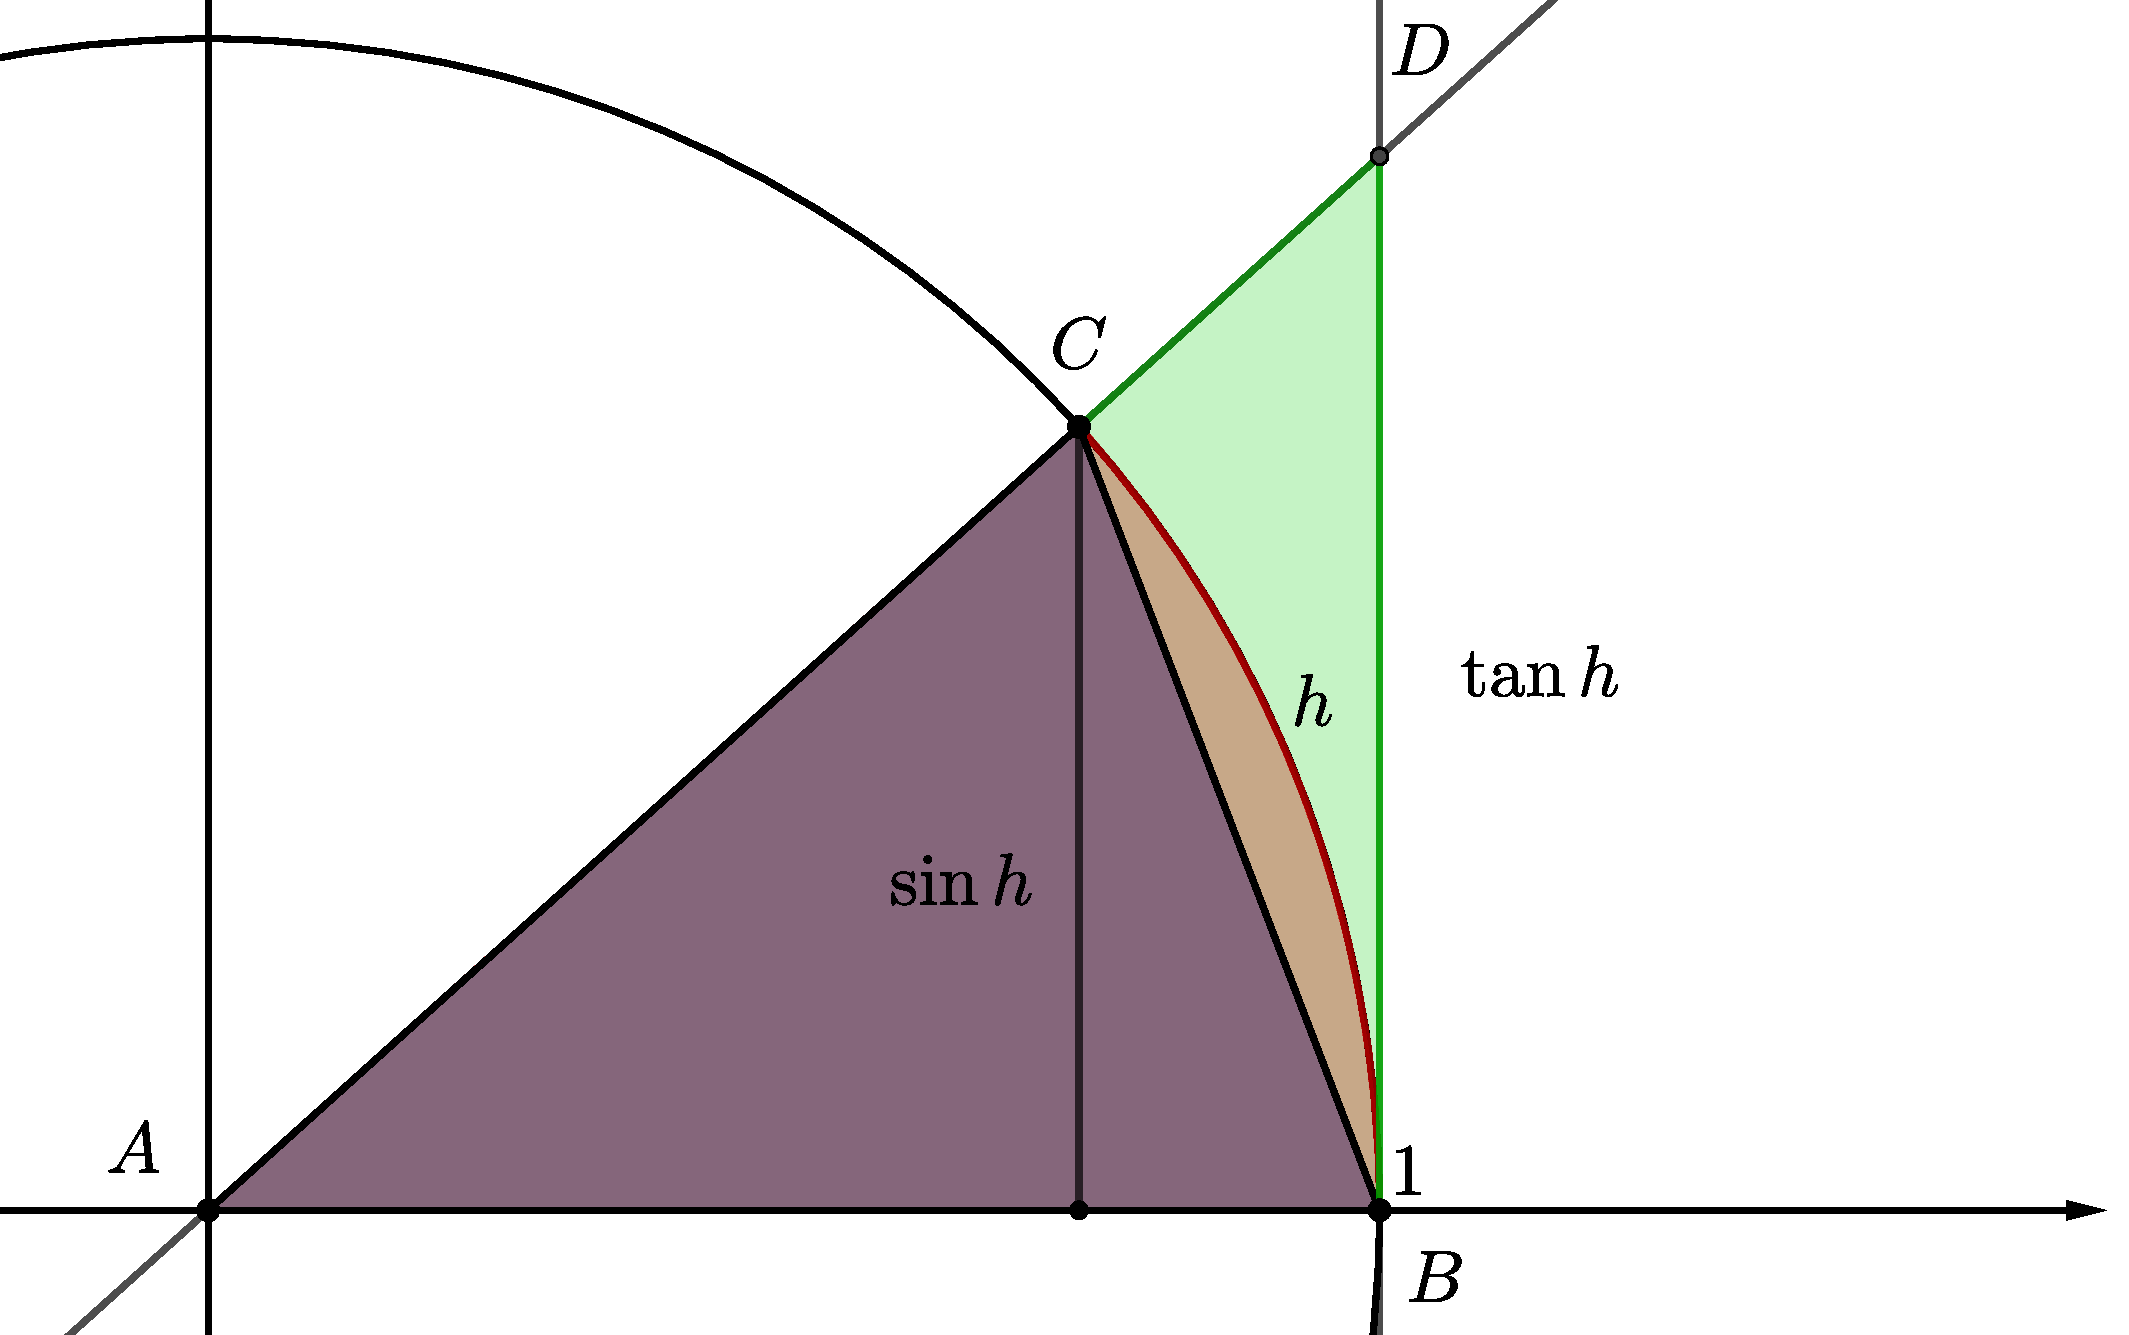
\includegraphics[width=0.7\textwidth]{grafici/sin_notevole}
		\caption{Le tre aree della disuguaglianza per la dimostrazione del limite notevole del seno.}
		\label{fig:dersin}
	\end{figure}
	Si nota che le aree del triangolo $ABC$, del settore circolare di angolo $h$, diciamo $S$ e del triangolo $ABD$ sono legate dalla relazione:
	\begin{equation}
		\label{dersin:dis}
		A_{ABC}<A_S<A_{ABD}
	\end{equation}
	La prima area vale $\frac{\overline{AB}*\sin h}{2}$, cioè, poiché $\overline{AB}=1$ per costruzione, $\frac{\sin h}{2}$. La terza area vale per lo stesso motivo $\frac{\tan h}{2}$. La seconda area invece è quella del settore circolare di angolo $h$, da cui per proporzionalità diretta con l'angolo giro vale:
	\[
		\frac{A_{\text{cerchio}}}{2\pi}=\frac{A_S}{h}
	\]
	Poiché l'area del cerchio unitario è $\pi\cdot 1^2=\pi$, $A_S=\frac{h}{2}$. La disuguaglianza \ref{dersin:dis} è quindi uguale a
	\[
		\frac{\sin h}{2}<\frac{h}{2}<\frac{\tan h}{2}
	\]
	Si moltiplica ora per $2$ e si divide per $\sin h$, che si sa essere positivo poiché $0<h<\frac{\pi}{2}$, per cui la disequazione mantiene il verso $<$:
	\begin{gather*}
		\frac{\sin h}{\sin h}<\frac{h}{\sin h}<\frac{\tan h}{\sin h}\\
		1<\frac{h}{\sin h}<\frac{1}{\cos h}
	\end{gather*}
	Poiché per $h\to0$ $\frac{1}{\cos h}$ tende a $1$, si applica il teorema del confronto (\vref{teor:confronto}) e si dimostra così che
	\[
		\lim_{h\to0^+} \frac{h}{\sin h}=\lim_{h\to0} \frac{\sin h}{h}=1
	\]
\end{proof}

\begin{teor}
	\label{deriv:cos}
	\[
		1-\cos h\sim \frac{h^2}{2}\qquad h\to0
	\]
\end{teor}
\begin{proof}
	In generale:
	\[
		1=\sin^2 h+\cos^2 h
	\]
	Per $h$ vicino a $0$ il coseno è positivo, quindi:
	\[
		\cos h=+\sqrt{1-\sin^2 h}
	\]
	Per il teorema precedente e per $h\to0$, $\sin h\sim h$, che in termini di $o$ piccolo equivale a $\sin h=h+o(h)$. Quindi l'uguaglianza equivale\footnote{si ricorda che nello sviluppo del quadrato $[h+o(h)]^2=h^2+2h*o(h)+[o(h)]^2$, il quadrato $[o(h)]^2$ è uguale a $o(h^2)$, mentre il doppio prodotto viene assorbito da $o(h^2)$} a
	\begin{equation}
		\label{eq:coseq}
		\cos h=\sqrt{1-[h+o(h)]^2}=\sqrt{1-h^2+o(h^2)}
	\end{equation}
	Traducendo il teorema \ref{deriv:nepero3} in termini di $o$ piccolo ($\varepsilon\to0$):
	\[
		(1+\varepsilon)^\alpha-1\sim\alpha\varepsilon\Rightarrow (1+\varepsilon)^\alpha-1=\alpha\varepsilon+o(\varepsilon)\Rightarrow (1+\varepsilon)^\alpha=1+\alpha\varepsilon+o(\varepsilon)
	\]
	applicato alla \ref{eq:coseq}, usando $\alpha=\frac{1}{2}$ e $\varepsilon=-h^2+o(h^2)$:
	\[
		\sqrt{1-h^2+o(h^2)}=1+\frac{1}{2}[-h^2+o(h^2)]+o[-h^2+o(h^2)]=
	\]
	Poiché $-h^2+o(h^2)\sim -h^2$:
	\[
		=1-\frac{1}{2}h^2+o(h^2)+o(h^2)=1-\frac{h^2}{2}+o(h^2)
	\]
	Riportandosi all'equazione iniziale:
	\[
		\cos h=1-\frac{h^2}{2}+o(h^2)\Rightarrow 1-\cos h=\frac{h^2}{2}+o(h^2)
	\]
	che tradotto in asintotico equivale a
	\[
		1-\cos h\sim\frac{h^2}{2}
	\]
\end{proof}

\subsubsection{Derivate elementari}
Calcoliamo ora, avvalendoci di tali teoremi, le derivate delle funzioni elementari:
\begin{itemize}
	\item $f(x)=\ln x$. Per $h\to0$:
	      \[
		      \frac{\ln (x_0+h)-\ln x_0}{h}=\frac{1}{h}\ln\left(\frac{x_0+h}{x_0}\right)=\frac{1}{h}\ln\left(1+\frac{h}{x_0}\right)
	      \]
	      Applicando il teorema \ref{deriv:nepero} con $\varepsilon=\frac{h}{x_0}$ (che tende a $0$):
	      \[
		      \frac{1}{h}\ln\left(1+\frac{h}{x_0}\right)\sim\frac{1}{h}\cdot \frac{h}{x_0}=\frac{1}{x_0}
	      \]
	\item $f(x)=\log_q x$. Considerato che, per cambio di base, $\log_q x=\log_q e\cdot \ln x_0$, il procedimento precedente può essere ripetuto con la costante moltiplicativa $\log_q e$, per cui la derivata sarà
	      \[
		      \frac{\log_q e}{x_0}
	      \]
	\item $f(x)=e^x$. Per $h\to0$:
	      \[
		      \frac{e^{x_0+h}-e^{x_0}}{h}=\frac{e^{x_0}e^h-e^{x_0}}{h}=e^{x_0}\frac{e^h-1}{h}
	      \]
	      Per il teorema \ref{deriv:nepero2}, con $\varepsilon=h\to0$:
	      \[
		      e^{x_0}\frac{e^h-1}{h}\sim e^{x_0}\frac{h}{h}=e^{x_0}
	      \]
	\item $f(x)=x^n$ con $n\in\N\setminus 0$. Per sviluppare la potenza della funzione incrementata si utilizza il binomio di Newton. Per $h\to0$:
	      \[
		      \frac{(x_0+h)^n-x_0^n}{h}=\frac{1}{h}\left[\left(\sum_{k=0}^n \binom{n}{k}h^k x_0^{n-k}\right)-x_0^n\right]
	      \]
	      Come si può intuire dallo sviluppo del teorema \ref{derivo}, sono i termini lineari in $h$ (cioè in cui $h$ è di primo grado) quelli a essere fondamentali per il calcolo della derivata; in particolare, tutti i termini che contengono $h$ elevato a esponenti maggiori o uguali a $2$ possono essere riassunti nel termine\footnote{con la semplificazione in $o(h)$ avviene una perdita di informazione, la cui però non ci è utile alla dimostrazione.} $o(h)$. La sommatoria può quindi essere semplificata in
	      \[
		      \frac{1}{h}\cdot \left[\left(x_0^n+\binom{n}{1}h x_0^{n-1}+o(h)\right)-x_0^n\right]=
	      \]
	      Sviluppando il coefficiente e ricordando che per definizione $\frac{o(h)}{h}=o(1)$:
	      \[
		      =\frac{x_0^n+nhx_0^{n-1}+o(h)-x_0^n}{h}=nx^{n-1}+o(1)\to nx^{n-1}
	      \]
	\item $f(x)=x^\alpha$, con $\alpha\in\R\land x\geq0$. Per $h\to0$:
	      \[
		      \frac{(x_0+h)^\alpha-x_0^\alpha}{h}=x_0^\alpha\cdot \frac{(1+\frac{h}{x_0})^\alpha-1}{h}
	      \]
	      Applicando il teorema \ref{deriv:nepero3}, con $\varepsilon=\frac{h}{x}\to0$:
	      \[
		      x_0^\alpha\cdot \frac{(1+\frac{h}{x_0})^\alpha-1}{h}\sim x^\alpha\cdot \frac{\alpha\frac{h}{x_0}}{h}\to\alpha x^{\alpha-1}
	      \]
	\item $f(x)=\sin x$. Utilizzando le formule goniometriche di addizione, per $h\to0$:
	      \begin{gather*}
		      \frac{\sin(x_0+h)-\sin x_0}{h}=\frac{\sin x_0\cos h+\cos x_0\sin h-\sin x_0}{h}=\\
		      \sin x_0 \cdot \frac{\cos h -1}{h}+\cos x_0 \cdot \frac{\sin h}{h}=
	      \end{gather*}
	      Applicando i teoremi \ref{deriv:sin} e \ref{deriv:cos}:
	      \[
		      =\sin x_0 \cdot \frac{-\frac{h^2}{2}}{h}+\cos x_0 \cdot \frac{h}{h}\to \cos x_0
	      \]
	\item $f(x)=\cos(x)$ Utilizzando le formule goniometriche di addizione, per $h\to0$:
	      \begin{gather*}
		      \frac{\cos(x_0+h)-\cos x_0}{h}=\frac{\cos x_0\cos h-\sin x_0\sin h-\cos x_0}{h}=\\
		      \cos x_0 \cdot \frac{\cos h -1}{h}-\sin x_0 \cdot \frac{\sin h}{h}=
	      \end{gather*}
	      Come nel caso precedente, si applicano i teoremi \ref{deriv:sin} e \ref{deriv:cos}:
	      \[
		      =\cos x_0 \cdot \frac{-\frac{h^2}{2}}{h}-\sin x_0 \cdot \frac{h}{h}\to-\sin x_0
	      \]
\end{itemize}


\subsection{Derivate non elementari}
Per calcolare la derivata di una funzione non elementare, è necessario ricavare metodi che permettano di calcolare la derivata di un'operazione tra funzioni (addizione, moltiplicazione, etc.). Questi metodi sono racchiusi in alcuni bteoremi. Le dimostrazioni di questi utilizzano per lo più lo sviluppo della funzione incrementata di cui al teorema \vref{derivo}.

\subsubsection{Derivata della somma}
\begin{prop}[Derivata della somma]
	Date due funzioni $f$ e $g$ derivabili in $x_0$:
	\[
		(f+g)'(x_0)=f'(x_0)+g'(x_0)
	\]
\end{prop}
\begin{proof}
	La somma incrementata delle due funzioni è, per lo sviluppo di cui al teorema \ref{derivo} (per $h\to0$):
	\begin{gather*}
		(f+g)(x_0+h)=f(x_0+h)+g(x_0+h)=\\
		(f(x_0)+f'(x_0)h+o(h))+(g(x_0)+g'(x_0)h+o(h))=\\
		=f(x_0)+g(x_0)+(f'(x_0)+g'(x_0))h+o(h)=\\
		(f+g)(x_0)+(f+g)'(x_0)h+o(h)
	\end{gather*}
	L'esistenza e la qualità dello sviluppo dimostra che la derivata è quella espressa dalla tesi.
\end{proof}
\begin{prop}[Derivata del prodotto]
	\label{der:prod}
	Date due funzioni $f$ e $g$ derivabili in $x_0$:
	\[
		(fg)'(x_0)=f(x_0)g'(x_0)+f'(x_0)g(x_0)
	\]
	La somma incrementata delle due funzioni è, per lo sviluppo di cui al teorema \ref{derivo} (per $h\to0$):
\end{prop}
\begin{proof}
	% TODO: aggiungere spiegazione o(h)
	\begin{gather*}
		(fg)(x_0+h)=f(x_0+h)g(x_0+h)=\\
		[f(x_0)+f'(x_0)h+o(h)][g(x_0)+g'(x_0)h+o(h)]=\\
		=f(x_0)g(x_0)+[f(x_0)g'(x_0)+f'(x_0)g(x_0)]h+o(h)
	\end{gather*}
\end{proof}

\begin{prop}
	% TODO: verificare ipotesi
	\label{der:reci}
	Data una funzione $f$ derivabile in $x_0$ tale che $f(x_0)\neq0$, allora $\frac{1}{f}$ è derivabile in $x_0$ e la sua derivata è uguale a:
	\[
		\left(\frac{1}{f}\right)'(x_0)=-\frac{f'(x_0)}{f^2(x_0)}
	\]
\end{prop}
\begin{proof}
	\begin{gather*}
		\left(\frac{1}{f}\right)(x_0+h)=\frac{1}{f(x_0+h)}=\frac{1}{f(x_0)+f'(x_0)h+o(h)}=\\
		\frac{1}{f(x_0)}\left(1+\frac{f'(x_0)}{f(x_0)}h+o(h)\right)^{-1}=
	\end{gather*}
	Si può applicare ora il limite notevole \ref{deriv:nepero3}, poiché $-\left(\frac{f'(x_0)}{f(x_0)}h+o(h)\right)$ è una quantità infinitesima:
	\[
		=\frac{1}{f(x_0)}\left[1-\left(\frac{f'(x_0)}{f(x_0)}h+o(h)\right)+o\left(-\left(\frac{f'(x_0)}{f(x_0)}h+o(h)\right)\right)\right]=
	\]
	L'argomento di $o$ è perlomeno $O(h)$, per cui l'intero termine $o(O(h))$ è uguale\footnote{Si veda il terzo punto della proprietà \ref{prop:landaugp}} a $o(h)$:
	\begin{gather*}
		=\frac{1}{f(x_0)}\left[1-\frac{f'(x_0)}{f(x_0)}h+o(h)+o(O(h))\right]=\frac{1}{f(x_0)}-\frac{f'(x_0)}{f^2(x_0)}h+o(h)
	\end{gather*}
\end{proof}

\begin{prop}
	Per $g(x_0)\neq0$:
	\[
		\left(\frac{f}{g}\right)'(x_0)=\frac{f'(x_0)g(x_0)-f(x_0)g'(x_0)}{g^2(x_0)}
	\]
\end{prop}
\begin{proof}
	Il quoziente $\frac{f}{g}$ non è altro che il prodotto di $f$ per il reciproco di $g$, quindi, per il teorema \ref{der:prod}:
	\[
		\left(\frac{f}{g}\right)'(x_0)=f'(x_0)\frac{1}{g(x_0)}+f(x_0)\left(\frac{1}{g(x_0)}\right)'=
	\]
	Per il teorema \ref{der:reci}:
	\[
		=f'(x_0)\frac{1}{g(x_0)}+f(x_0)\left(-\frac{g'(x_0)}{g^2(x_0)}\right)=\frac{f'(x_0)g(x_0)-f(x_0)g'(x_0)}{g^2(x_0)}
	\]
\end{proof}

\begin{prop}[Derivata di funzione composta]
	\label{der:comp}
	\[
		\begin{cases}
			g \text{ derivabile in $x_0$} \\
			f \text{ derivabile in $g(x_0)$}
		\end{cases}\Rightarrow
		\begin{cases}
			(f\circ g)(x_0)\text{ derivabile in $x_0$} \\
			(f\circ g)'(x_0)=f'(g(x_0))g'(x_0)
		\end{cases}
	\]
\end{prop}
\begin{proof}
	Per $h\to0$
	\begin{equation*}
		(f\circ g)(x_0+h)=f(g(x_0+h))=f(g(x_0)+\underbrace{g'(x_0)h+o(h)}_{k})=
	\end{equation*}
	La quantità $k=g'(x_0)h+o(h)$ tende a $0$ per $h\to0$. L'espressione può essere dunque vista come la funzione incrementata $f(g(x_0)+k)$. Sfruttando l'ipotesi della deribabilità di $f$ in $g(x_0)$, si può scrivere lo sviluppo:
	\begin{gather*}
		f(g(x_0))+f'(g(x_0))[g'(x_0)h+o(h)]+o(g'(x_0)h+o(h)) = \\
		(f\circ g)(x_0)+f'(g(x_0))g'(x_0)h+\underbrace{f'(g(x_0))o(h)+o(g'(x_0)h+o(h))}_{o(h)} = \\
		(f\circ g)(x_0)+f'(g(x_0))g'(x_0)h+o(h)
	\end{gather*}
\end{proof}

\begin{prop}[Derivata dell'inversa]
	Per $f'(x_0)\neq0$:
	\[
		Df^{-1}(y)=\frac{1}{Df(f^{-1}(y))}
	\]
\end{prop}
\begin{proof}
	Poiché $f^{-1}(y)$ è l'inversa di $f(y)$, si verifica che $f(f^{-1}(y))=y$. Utilizzando il teorema \ref{der:comp} per le funzioni composte:
	\[
		D(f(f^{-1}(y)))=Df(f^{-1}(y))\cdot Df^{-1}(y)
	\]
	Questa derivata è uguale a $1$ in quanto la funzione è uguale a $y$ per ogni $y$. Questo ci permette di ricavare la derivata della funzione inversa, ovvero il secondo fattore:
	\[
		Df^{-1}(y)=\frac{1}{Df(f^{-1}(y))}
	\]
\end{proof}

\begin{examp}
	La derivata dell'arcotangente, definita come la funzione inversa della tangente per l'intervallo $-\frac{\pi}{2},\frac{\pi}{2}$, si può calcolare applicando il teorema appena dimostrato:
	\[
		D\arctan y=\frac{1}{\tan'(\arctan y)}=\cos^2(\arctan y)
	\]
	Chiamiamo $\theta=\arctan y$. Dividendo il risultato per $1=\sin^2\theta+\cos^2\theta$:
	\[
		\frac{\cos^2\theta}{\sin^2\theta+\cos^2\theta}=\frac{1}{\frac{\sin^2\theta+\cos^2\theta}{\cos^2\theta}}=\frac{1}{\tan^2\theta+1}
	\]
	Poiché $\tan\theta=\tan(\arctan y)=y$:
	\[
		D\arctan y=\frac{1}{y^2+1}
	\]
\end{examp}

\section{Teoremi sulle derivate}
I seguenti teoremi riguardano il rapporto tra alcuni punti di funzioni che godono di proprietà particolari e le relative derivate. Tra questi punti:
\begin{defin}
	Data una funzione $f:D\to\R$, si definisce:
	\begin{description}
		\item[Punto di massimo relativo] (o locale) un punto $x_0$ tale che
			\[
				\exists U\in I(x_0)\mid\forall x\in U: f(x)\leq f(x_0)
			\]
		\item[Punto di minimo relativo] (o locale) un punto $x_0$ tale che
			\[
				\exists U\in I(x_0)\mid\forall x\in U: f(x)\geq f(x_0)
			\]
		\item[Punto di massimo assoluto] (o globale) un punto $x_0$ tale che
			\[
				\forall x\in D: f(x)\leq f(x_0)
			\]
		\item[Punto di minimo assoluto] (o globale) un punto $x_0$ tale che
			\[
				\forall x\in D: f(x)\geq f(x_0)
			\]
	\end{description}
	Ognuno di questi ha una variante ``stretta'', cioè che non contempla la possibilità che $f(x_0)=f(x)$ (in questo caso $x\neq x_0$). Massimi e minimi sono detti estremi (relativi o assoluti).
\end{defin}


\subsection{Teorema di Fermat}
Il teorema di Fermat permette di associare in alcuni casi la presenza di un estremo relativo all'azzeramento della derivata. Esso segue (e in un certo senso unisce) due lemmi:
\begin{lemma}[Minimalità locale destra]
	\label{fermat:lemma1}
	\[
		\begin{cases}
			\exists\delta>0\mid f(x)\geq f(x_0)~\forall x\in[x_0,x_0+\delta) \\
			\exists D^+f(x_0)
		\end{cases}\Rightarrow
		D^+f(x_0)\geq0
	\]
\end{lemma}
\begin{proof}
	Per definizione:
	\[
		D^+f(x_0)=\lim_{x\to x_0^+}\frac{f(x)-f(x_0)}{x-x_0}
	\]
	Studiando il segno di questa frazione, si può dire che il denominatore è sempre positivo (poiché $x\to x_0^+$); inoltre, il numeratore è anch'esso positivo in quanto, per ipotesi, $f(x)\geq f(x_0)$, a patto di prendere un $x$ appartenente a $[x_0,x_0+\delta)$. È immediato concludere che il limite è maggiore o uguale a $0$.
\end{proof}
\begin{lemma}[Minimalità locale sinistra]
	\label{fermat:lemma2}
	\[
		\begin{cases}
			\exists\delta>0\mid f(x)\geq f(x_0)~\forall x\in(x_0-\delta,x_0] \\
			\exists D^-f(x_0)
		\end{cases}\Rightarrow
		D^+f(x_0)\leq0
	\]
\end{lemma}
\begin{proof}
	Valgono le stesse considerazioni del caso precedente, questa volta per un denominatore minore di $0$ (poiché $x\to x_0^-$) e un numeratore maggiore di $0$, a patto di prendere un $x$ appartenente a $(x_0-\delta,x_0]$.
\end{proof}

Unendo i due lemmi nel caso di esistenza della derivata bilaterale si ottiene il teorema di Fermat:
\begin{teor}[di Fermat]
	La derivata di una funzione in un punto di massimo relativo è $0$, se la funzione è derivabile in quel punto.
	\[
		\begin{cases}
			\exists\delta>0\mid f(x)\geq f(x_0)\forall x\in(x_0-\delta,x_0+\delta) \\
			\exists Df(x_0)
		\end{cases}\Rightarrow
		Df(x_0)=0
	\]
\end{teor}
Analogo vale per i punti di minimo relativo.
\begin{proof} ~
	\begin{itemize}
		\item Tutte le ipotesi del lemma \ref{fermat:lemma1} sono verificate, per cui:
		      \[
			      D^+f(x_0)\geq0
		      \]
		\item Tutte le ipotesi del lemma \ref{fermat:lemma2} sono verificate, per cui:
		      \[
			      D^-f(x_0)\leq0
		      \]
	\end{itemize}
	Poiché la derivata bilaterale esiste, la derivata destra e quella sinistra devono essere uguali. L'unico caso in cui ciò è possibile è quello in cui $Df(x_0)=0$
\end{proof}
\begin{defin}[punto stazionario]
	Un punto è stazionario per una funzione se e solo se la sua derivata in tale punto è $0$.
\end{defin}


\subsection{Teorema di Rolle}
\begin{teor}[di Rolle]
	\label{der:rolle}
	Data una funzione $f:[a,b]\to\R$
	\[
		\begin{cases}
			f\text{ continua in } [a,b]   \\
			f\text{ derivabile in } (a,b) \\
			f(a)=f(b)
		\end{cases}\Rightarrow
		\exists c\in(a,b)\mid f'(c)=0
	\]
\end{teor}
\begin{proof}
	% TODO: ref al teorema di Weierstrass una volta aggiunto
	Per il teorema di Weierstrass, essendo $f$ continua:
	\[
		f(x_m)\leq f(x)\leq f(x_M)\qquad\forall x\in[a,b]
	\]
	Si possono verificare due casi:
	\begin{itemize}
		\item se $x_m\in(a,b)\lor x_M\in(a,b)$, poiché la funzione è derivabile in tale intervallo è possibile applicare il teorema di Fermat al punto interessato, che sarà dunque il $c$ che si cercava;
		\item se $x_m,x_M\in\{a,b\}$, allora $f(a)\leq f(x)\leq f(b)\qquad\forall x\in[a,b]$. Poiché per ipotesi $f(a)=f(b)$ la funzione è costante e pertanto la derivata è $0$ in qualunque punto $c=x$ interno a $(a,b)$.
	\end{itemize}
\end{proof}


\subsection{Teorema di Lagrange}
\begin{teor}[di Lagrange]
	\label{der:lagrange}
	Data una funzione $f:[a,b]\to\R$:
	\[
		\begin{cases}
			f\text{ continua in } [a,b] \\
			f\text{ derivabile in } (a,b)
		\end{cases}\Rightarrow
		\exists c\in(a,b)\mid f'(c)=\frac{f(b)-f(a)}{b-a}
	\]
\end{teor}
% TODO: grafico
\begin{proof}
	Da un punto di vista geometrico, il rapporto $\frac{f(b)-f(a)}{b-a}$ non è altro che il coefficiente angolare della retta $r$, secante a $f$, passante per $a$ e $b$. Poiché la derivata di una funzione in un punto è uguale al coefficiente angolare della retta tangente in quel punto, la tesi può essere tradotta nell'esistenza di un punto interno all'intervallo in cui la tangente è parallela alla congiungente $ab$.

	Per dimostrare il teorema ci si riconduce ai casi contemplati dal teorema di Rolle, utilizzando una funzione ausiliaria $g$, definita come la differenza, nel punto $x$, tra la funzione $f$ e la retta $r$. Questa funzione, in quanto differenza di una funzione continua e derivabile per ipotesi e una retta (continua e derivabile per ogni $x$), è continua e derivabile nell'intervallo; inoltre per costruzione $g(a)=g(b)=0$. Applicando il teorema \ref{der:rolle} di Rolle si ottiene:
	\[
		\exists c\in(a,b)\mid g'(c)=0
	\]
	Ma $g'(x)$ non è altro che la derivata di una differenza, quindi:
	\[
		g'(x)=f'(x)-r'(x)
	\]
	Poiché la derivata di $r$ è nota e $g'(c)=0$:
	\[
		f'(c)=r'(c)\Rightarrow f'(c)=\frac{f(b)-f(a)}{b-a}
	\]
\end{proof}

\subsection[Funzioni monotone]{Caratterizzazione differenziale di funzioni monotone}
\label{der:monotone}
\begin{prop}
	Date le ipotesi
	\[
		\begin{cases}
			I=(a,b)\subseteq\R                   \\
			f:I\to\R \text{ continua in $[a,b]$} \\
			f:I\to\R \text{ derivabile in $(a,b)$}
		\end{cases}
	\]
	Allora
	\[
		\begin{cases}
			\bullet~ f \text{ crescente in senso lato in $I$} & \iff f'(x)\geq0~\forall x\in I                        \\
			\bullet~ f \text{ strettamente crescente in $I$}  & \iff f'(x)\geq0~\forall x\in I\land                   \\
			                                                  & \{x\in I\mid f'(x)=0\}\text{ non contiene intervalli}
		\end{cases}
	\]
\end{prop}
E l'opposto vale per funzioni decrescenti.
\begin{proof}
	Dimostriamo la prima relazione verso destra. La derivata in $x_0$ è così definita
	\[
		\lim_{x\to x_0}\frac{f(x)-f(x_0)}{x-x_0}
	\]
	Per la definizione di funzione crescente in un intervallo, comunque scelto $x\in I$ vale la relazione: $x>x_0\Rightarrow f(x)\geq f(x_0)$. Ciò significa che quando il denominatore è positivo lo è anche il numeratore e viceversa. In conclusione, la derivata è maggiore o uguale a $0$ in ogni punto dell'intervallo.

	L'implicazione inversa richiede l'applicazione del teorema di Lagrange. Dimostrare la tesi significa dimostare che comunque scelti due valori $x_1<x_2$ nell'intervallo vale $f(x_1)<f(x_2)$. Poiché $x_1$ e $x_2$ appartengono all'intervallo, sono verificate tutte le ipotesi del teorema di Lagrange, quindi:
	\[
		\exists c\in I\mid f'(c)=\frac{f(x_2)-f(x_1)}{x_2-x_1}
	\]
	Manipolando l'espressione:
	\[
		(x_2-x_1)f'(c)=f(x_2)-f(x_1)
	\]
	Poiché $f'(c)\geq0$ per ipotesi e $x_2-x_1>0$ per costruzione, il primo membro è non negativo, e quindi anche il secondo membro deve esserlo. Questo significa che $f(x_2)\geq f(x_1)$.

	Per quanto riguarda la seconda relazione, essa deve escludere dal caso precedente i casi in cui, scelti $x_1<x_2$ nell'intervallo, vale $f(x_1)=f(x_2)$. Se così fosse infatti, varrebbe:
	% TODO: spiegare meglio. Occorre dimostrare che l'unico caso in cui una derivata è nulla in un certo intervallo è quello in cui la funzione è costante
	\[
		\begin{cases}
			f(x_1)=f(x_2) \\
			f(x_1)\leq f(x)\leq f(x_2)~\forall x\in [x_1,x_2]
		\end{cases}\Rightarrow f(x_1)=f(x)=f(x_2)~\forall x\in [x_1,x_2]
	\]
	ovvero, la funzione sarebbe costante nell'intervallo $[x_1,x_2]$. Ergo, deve valere $f'(x)\geq0$ ma non può valere $f'(x)=0$ per alcun intervallo\footnote{La precauzione di non usare $f'(x)>0\forall x\in I$ deriva dal fatto che la derivata di una funzione strettamente crescente può essere nulla in punti isolati, i flessi a tangente orizzontale (si pensi ad esempio a $y=x^3$ in $x=0$).}.
\end{proof}

\subsection{Teorema di Cauchy}
Il teorema di Cauchy generalizza ulteriormente quello di Lagrange.
\begin{teor}[di Cauchy]
	\label{der:cauchy}
	Date due funzioni $f,g:[a,b]\to\R$
	\[
		\begin{cases}
			f,g \text{ continue in }[a,b]   \\
			f,g \text{ derivabili in }(a,b) \\
			g'(x)\neq0\quad\forall x\in(a,b)
		\end{cases}\Rightarrow
		\exists c\in(a,b)\mid\frac{f'(c)}{g'(c)}=\frac{f(b)-f(a)}{g(b)-g(a)}
	\]
\end{teor}
\begin{proof}
	Come nella dimostrazione del teorema \ref{der:lagrange} di Lagrange, si utilizza una funzione ausiliaria. Questa volta, essa non ha una rappresentazione grafica immediata, ma sono evidenti le somiglianze con la precedente.
	\[
		h(x)=f(x)-\left\{f(a)+\frac{f(b)-f(a)}{g(b)-g(a)}(g(x)-g(a))\right\}
	\]
	Anche qui si applica il teorema di \ref{der:rolle} Rolle, infatti:
	\begin{gather*}
		\begin{cases}
			h(a)=f(a)-\{f(a)+0\}=0 \\
			h(b)=f(b)-\left\{f(a)+\dfrac{f(b)-f(a)}{g(b)-g(a)}(g(b)-g(a))\right\}=0
		\end{cases}\Rightarrow\\
		\Rightarrow\exists c\in(a,b)\mid h'(c)=0
	\end{gather*}
	Eguagliando la derivata in $c$ di $h$ a $0$ (i termini non dipendenti da $c$ contano come costanti):
	\begin{gather*}
		0=f'(c)-\left\{0+\frac{f(b)-f(a)}{g(b)-g(a)}(g'(c)-0)\right\}\\
		0=f'(c)-\frac{f(b)-f(a)}{g(b)-g(a)}g'(c)\\
		\frac{f'(c)}{g'(c)}=\frac{f(b)-f(a)}{g(b)-g(a)}
	\end{gather*}
	Si noti che la condizione $g'(x)\neq0$ non solo certifica l'esistenza di $\frac{f'(x)}{g'(x)}$, ma anche quella di $\frac{f(b)-f(a)}{g(b)-g(a)}$. Infatti, se il denominatore fosse nullo e quindi $g(a)=g(b)$, il teorema di Rolle implicherebbe l'esistenza di un $c$ per cui $g'(c)=0$, cosa impossibile per ipotesi.
\end{proof}


\subsection{Teorema di De L'Hôpital}
\begin{teor}[di De L'Hôpital]
	\label{der:hopital}
	Per $x_0\in\Rt$, se
	\[
		\begin{cases}
			\exists U\in I(x_0)\mid f,g\text{ derivabili in }U                                                                               \\
			g'(x)\neq0~\forall x\in U                                                                                                        \\
			\lim_{x\to x_0}\limits f(x)=\lim_{x\to x_0}\limits g(x)=0\lor \lim_{x\to x_0}\limits f(x) =\lim_{x\to x_0}\limits g(x)=\pm\infty \\
			\exists \lim_{x\to x_0}\limits \frac{f'(x)}{g'(x)}=L
		\end{cases}
	\]
	allora:
	\[
		\exists\lim_{x\to x_0} \frac{f(x)}{g(x)}=L
	\]
\end{teor}
\begin{proof}
	Per semplicità, si dimostra il teorema nel caso di indecisione $0/0$ per $x\to x_0\in\R$. Poiché la funzione $f$ è derivabile e quindi continua in $x_0$, vale $\lim{x\to x_0}f(x)=f(x_0)$. Lo stesso vale per $g$. Poiché questi limiti in questo caso valgono $0$, vale:
	\[
		\frac{f(x)}{g(x)}=\frac{f(x)-f(x_0)}{g(x)-g(x_0)}
	\]
	Applicando il teorema \ref{der:cauchy} di Cauchy:
	\[
		\exists c\mid \frac{f'(c)}{g'(c)}=\frac{f(x)-f(x_0)}{g(x)-g(x_0)}
	\]
	Poiché $c$ appartiene all'intervallo $(x_0,x)$, per il teorema del confronto per $x\to x_0$ vale $c\to x_0$, quindi:
	\begin{equation*}
		\lim_{x\to x_0} \frac{f'(x)}{g'(x)}=\lim_{c\to x_0} \frac{f'(c)}{g'(c)}=\lim_{x\to x_0} \frac{f(x)-f(x_0)}{g(x)-g(x_0)}=\lim_{x\to x_0} \frac{f(x)}{g(x)}=L
	\end{equation*}
\end{proof}

%% Copyright (C) 2019-2021 Alessandro Clerici Lorenzini
%
% This work may be distributed and/or modified under the
% conditions of the LaTeX Project Public License, either version 1.3
% of this license or (at your option) any later version.
% The latest version of this license is in
%   http://www.latex-project.org/lppl.txt
% and version 1.3 or later is part of all distributions of LaTeX
% version 2005/12/01 or later.
%
% This work has the LPPL maintenance status `maintained'.
%
% The Current Maintainer of this work is Alessandro Clerici Lorenzini
%
% This work consists of the files listed in work.txt


\section{Sviluppi di Taylor}

\subsection{Teorema di Taylor}
Lo scopo del teorema di Taylor è quello di approssimare una funzione $f$ in un centro $x_0$ (cioè per $x\to x_0$) tramite un polinomio. Lo sviluppo più semplice è dato da una costante più una quantità che tende a $0$:
\begin{equation}
	\label{taylor0}
	f(x)=a_0+o(1)\qquad x\to x_0
\end{equation}
Per aumentare la precisione si esplicita una quantità che dipende da $x$ e tende a $0$:
\begin{equation}
	\label{taylor1}
	f(x)=a_0+a_1(x-x_0)+o(x-x_0)
\end{equation}
Il procedimento viene ripetuto un numero arbitrario di volte, ottenendo un'approssimazione sempre migliore della funzione:
\begin{gather}
	\label{taylor2}
	f(x)=a_0+a_1(x-x_0)+a_2(x-x_0)^2+o((x-x_0)^2)\\
	\label{taylor3}
	f(x)=a_0+a_1(x-x_0)+a_2(x-x_0)^2+a_3(x-x_0)^3+o((x-x_0)^3)\\
	\dots\notag
\end{gather}
A ogni passaggio si aggiunge un coefficiente. Questi coefficienti, come si vedrà, sono unici e quindi uguali tra passaggi.

Per esprimere la funzione nella forma (\ref{taylor0}) è necessario partire dall'ipotesi che $f$ sia continua in $x_0$. Infatti, in tal caso:
\[
	f(x)=f(x_0)+o(1)
\]
Ovvero $a_0=f(x_0)$. A partire dalla (\ref{taylor1}) è necessario che $f$ sia derivabile. Infatti, al fine di calcolare $a_1$:
\begin{gather*}
	f(x)=f(x_0)+a_1(x-x_0)+o(x-x_0)\\
	f(x)-f(x_0)=a_1(x-x_0)+o(x-x_0)\\
	\frac{f(x)-f(x_0)}{(x-x_0)}=a_1+\frac{o(x-x_0)}{(x-x_0)}
\end{gather*}
Calcolando il limite per $x\to x_0$ (e usando le definizioni di $o$ e di derivata):
\[
	f'(x_0)=a_1+0
\]
Quindi $a_1=f'(x_0)$. Si procede per la (\ref{taylor2}), supponendo questa volta che $f$ sia derivabile due volte in $x_0$:
\begin{gather*}
	f(x)=f(x_0)+f'(x_0)(x-x_0)+a_2(x-x_0)^2+o((x-x_0)^2)\\
	f(x)-[f(x_0)+f'(x_0)(x-x_0)]=a_2(x-x_0)^2+o((x-x_0)^2)\\
	\frac{f(x)-[f(x_0)+f'(x_0)(x-x_0)]}{(x-x_0)^2}=a_2+\frac{o((x-x_0)^2)}{(x-x_0)^2}\\
	\lim_{x\to x_0}\frac{f(x)-[f(x_0)+f'(x_0)(x-x_0)]}{(x-x_0)^2}=a_2+\lim_{x\to x_0}\frac{o((x-x_0)^2)}{(x-x_0)^2}
\end{gather*}
Mentre il limite al secondo membro vale $0$ per definizione, al primo limite si può applicare il teorema \ref{der:hopital} di De l'Hôpital, infatti sia il numeratore che il denominatore tendono a $0$:
\begin{gather*}
	a_2=\lim_{x\to x_0}\frac{f(x)-[f(x_0)+f'(x_0)(x-x_0)]}{(x-x_0)^2}=\\
	=\lim_{x\to x_0}\frac{f'(x)-[0+f'(x_0)]}{2(x-x_0)}=\frac{f''(x_0)}{2}
\end{gather*}
Quindi $a_2 = \frac{f''(x_0)}{2}$. Per quanto riguarda lo sviluppo \ref{taylor3}, supponendo che $f$ sia derivabile tre volte in $x-0$:
\begin{dmath*}
	f(x) = f(x_0)+f'(x_0)(x-x_0)+\frac{f''(x_0)}{2}(x-x_0)^2+a_3(x-x_0)^3+o((x-x_0)^3)
\end{dmath*}
\begin{dmath*}
	f(x)-\left[f(x_0)+f'(x_0)(x-x_0) + \frac{f''(x_0)}{2}(x-x_0)^2\right] = a_3(x-x_0)^3+o((x-x_0)^3)
\end{dmath*}
\begin{equation*}
	\lim_{x\to x_0}\frac{f(x)-\left[f(x_0)+f'(x_0)(x-x_0)+\frac{f''(x_0)}{2}(x-x_0)^2\right]}{(x-x_0)^3}=a_3+0
\end{equation*}
Applicando De L'Hôpital:
\begin{gather*}
	\lim_{x\to x_0}\frac{f(x)-\left[f(x_0)+f'(x_0)(x-x_0)+\frac{f''(x_0)}{2}(x-x_0)^2\right]}{(x-x_0)^3}=\\
	=\lim_{x\to x_0}\frac{f'(x)-\left[0+f'(x_0)+f''(x_0)(x-x_0)\right]}{3(x-x_0)^2}=
\end{gather*}
Applicando nuovamente De L'Hôpital:
\[
	=\lim_{x\to x_0}\frac{f''(x)-[0+f''(x_0)]}{3*2(x-x_0)}=\frac{f'''(x_0)}{3*2}
\]
Da cui $a_3=\frac{f'''(x_0)}{3*2}$. Come si può notare il denominatore cresce fattorialmente.

\begin{teor}[di Taylor]
	\label{der:taylor}
	Data una funzione $f$ derivabile $n$ volte in $x_0$, per $x\to x_0$:
	\[
		\exists! P_n(x-x_0), \text{grado}(P_n)\leq n\mid f(x)=P_n(x-x_0)+o((x-x_0)^n)
	\]
	Dove $P_n$ è un polinomio così costruito:
	\[
		P_n(x-x_0)=f(x_0)+\sum_{k=1}^n \frac{D^kf(x_0)}{k!}(x-x_0)^k
	\]
	e $R_n(x)=o((x-x_0)^n)$ è detto resto di Teano.
\end{teor}


\subsection{Resto secondo Lagrange}
\begin{teor}
	\label{tay:restolagrange}
	Data una funzione $f:U\in I(x_0)\to\R$, derivabile in tutto l'intervallo, eccetto al più $x_0$, $n+1$ volte:
	\[
		\forall x\in I\exists c\in I\setminus\{x_0\}\mid R_n(x)=\frac{D^{n+1}f(c)}{(n+1)!}(x-x_0)^{n+1}
	\]
	Dove $R_n(x)$ è il resto dello sviluppo di Taylor centrato in $x_0$ della funzione $f$.
\end{teor}
\begin{proof}
	Si dimostra il caso in cui $x>x_0$. Il caso complementare è del tutto analogo.

	Per definizione il resto $R_n(x)$ è
	\[
		R_n(x)=f(x)-P_n(x-x_0)
	\]
	Inoltre definiamo
	\[
		G_n(x)=(x-x_0)^{n+1}
	\]
	Si noti che queste due funzioni sono derivabili $n+1$ volte nell'intervallo: $R_n(x)$ poiché è la differenza di una funzione derivabile per ipotesi e un polinomio di grado $n$ e $G_n(x)$ perché è un polinomio di grado $n+1$. Inoltre in $x_0$ la funzione $G_n(x)$ è $0$, poiché ogni termine contenente $(x-x_0)$ del polinomio di Taylor si annulla:
	\[
		R_n(x_0)=f(x_0)-f(x_0)-\frac{f'(x_0)}{1}(x_0-x_0)-\dots-\frac{D^n(x_0)}{n!}(x_0-x_0)^n=0
	\]
	Lo stesso vale per ogni sua derivata fino all'$n$-esima, poiché $f(x)$ viene derivata, il polinomio scende a ogni passaggio di un grado, elidendo la costante iniziale e fornendone una nuova (ed elidendo il coefficiente fattoriale con quello ottenuto dalla derivazione). Come si può più facilmente verificare, il resto nella forma di Teano è $o((x-x_0)^n)$, il cui unico sviluppo di Taylor di ordine $n$ in $x_0$ è
	\[
		0+o((x-x_0)^n)
	\]
	Dove ogni derivata è nulla. Lo stesso non vale per la derivata $n+1$-esima, poiché il polinomio di Taylor è di grado $n$, e viene quindi annullato alla $n+1$-esima derivazione:
	\begin{equation}
		\label{relag:R}
		D^{n+1}R_n(x)=D^{n+1}f(x)-0\qquad\forall x\in I
	\end{equation}
	La funzione $G_n(x)$ invece derivata $n+1$ volte in $x_0$ vale
	\begin{gather}
		G_n(x)=(x-x_0)^{n+1}\notag\\
		G'_n(x)=(n+1)(x-x_0)^n\notag\\
		G''_n(x)=n(n+1)(x-x_0)^{n-1}\notag\\
		\dots\notag\\
		\label{relag:G}
		D^{n+1}G_n(x)=(n+1)!\qquad\forall x\in I
	\end{gather}
	Per $x=x_0$ ogni derivata fino all'$n+1$-esima esclusa è quindi nulla.

	Le funzioni $R_n(x)$ e $G_n(x)$ soddisfano le ipotesi del teorema di Cauchy (\ref{der:cauchy}) nell'intervallo $[x_0,x]$ (per ovvi motivi), quindi:
	\[
		\exists c_1\in(x_0,x)\mid\frac{R_n(x)-R_n(x_0)}{G_n(x)-G_n(x_0)}=\frac{DR_n(c_1)}{DG_n(c_1)}
	\]
	E poiché $R_n(x_0)=G_n(x_0)=0$:
	\[
		\frac{R_n(x)}{G_n(x)}=\frac{R_n(c_1)}{G_n(c_1)}
	\]
	Ma ora $DR_n$ e $DG_n$ soddisfano le ipotesi del teorema di Cauchy nell'intervallo $[x_0,c_1]$, quindi:
	\[
		\exists c_2\in(x_0,c_1)\mid\frac{DR_n(c_1)-DR_n(x_0)}{DG_n(c_1)-DR_n(c_1)}=\frac{D^2R_n(c_2)}{D^2G_n(c_2)}
	\]
	E poiché $DR_n(x_0)=DG_n(x_0)=0$:
	\[
		\frac{R_n(x)}{G_n(x)}=\frac{DR_n(c_1)}{DG_n(c_1)}=\frac{D^2R_n(c_2)}{D^2G_n(c_2)}
	\]
	Così procedendo $n$ volte si giunge a:
	\[
		\frac{R_n(x)}{G_n(x)}=\frac{D^nR(c_n)}{D^nG(c_n)}
	\]
	Applicando un'ultima volta Cauchy all'intervallo $(x_0,c_n)$:
	\[
		\exists c\in(x_0,c_n)\mid\frac{R_n(x)}{G_n(x)}=\frac{D^{n+1}R(c)}{D^{n+1}G(c)}
	\]
	Queste derivate, come dimostrato precedentemente (equazioni \ref{relag:R} e \ref{relag:G}), valgono:
	\begin{gather*}
		D^{n+1}R(c)=D^{n+1}f(c)\\
		D^{n+1}G(c)=(n+1)!
	\end{gather*}
	Quindi, ricordando che $G_n(x)=(x-x_0)^{n+1}$:
	\[
		\frac{R_n(x)}{(x-x_0)^{n+1}}=\frac{D^{n+1}f(c)}{(n+1)!}
	\]
	Ovvero:
	\[
		R_n(x)=\frac{D^{n+1}f(c)}{(n+1)!}(x-x_0)^{n+1}
	\]

	Raramente questa forma viene usata in modo quantitativo, poiché sarebbe necessario determinare un $c$. Tuttavia, essa può essere scritta nella ben più utilizzata forma qualitativa (la cui dimostrazione è immediata):
	\[
		R_n(x)=O((x-x_0)^{n+1})
	\]
\end{proof}


\subsection{Taylor per i punti stazionari}
Il teorema di Taylor può essere applicato nella determinazione dei punti stazionari e della loro qualità.
\begin{teor}
	Se una funzione $f$, derivabile $k$ volte, è scrivibile per $x\to x_0$ nella forma:
	\[
		f(x)=f(x_0)+\frac{D^k(x_0)}{k!}(x-x_0)^k+o((x-x_0)^k)\qquad k\geq2
	\]
	Allora $x_0$ è un punto stazionario e in particolare, se $k$ è pari sarà un punto di estremo, se $k$ è dispari sarà un flesso a tangente orizzontale.
\end{teor}
\begin{proof}
	Si noti che l'ipotesi corrisponde a uno sviluppo di Taylor per $x\to x_0$ in cui ogni derivata dalla prima alla $k-1$-esima sono nulle, mentre la $k$-esima è diversa da zero. Poiché la derivata prima è nulla (infatti $k\geq2$ per ipotesi), il punto è stazionario. La vera utilità del teorema sta però nel ricavare la natura di questi punti. Portando a sinistra $f(x_0)$:
	\begin{gather*}
		f(x)-f(x_0)=\frac{D^k(x_0)}{k!}(x-x_0)^k+o((x-x_0)^k)\\
		f(x)-f(x_0)=\frac{D^k(x_0)}{k!}(x-x_0)^k[1+o(1)]
	\end{gather*}
	Studiare il segno di $f(x)-f(x_0)$ significa studiare la quota relativa di $f(x)$ rispetto a $f(x_0)$ in un intorno di $x_0$. Poiché è verificata l'uguaglianza, questa operazione è equivalente a determinare il segno del secondo membro. Poiché $1+o(1)$ è definitivamente positivo per $x\to x_0$ e $k!$ è sempre positivo, il segno dipende solamente da
	\[
		D^k(x_0)(x-x_0)^k
	\]
	\begin{itemize}
		\item Se $k$ è pari, il secondo fattore è positivo, per cui il segno globale sarà uguale in un intorno destro e sinistro di $x_0$, concorde con $D^k(x_0)$ (che chiaramente rimane invariato essendo una costante). In particolare, se $D^k(x_0)>0$ il segno sarà positivo per l'intorno di $x_0$ (nullo in $x_0$ stesso), quindi la quota relativa sarà positiva e il punto sarà di minimo; se $D^k(x_0)<0$ allora il segno della quota relativa sarà negativo sia a destra sia a sinistra di $x_0$, facendo del punto un punto di massimo;
		\item Nel caso di $k$ dispari invece, il segno della quota relativa sarà asimmetrico, ovvero $x_0$ sarà un flesso a tangente orizzontale, crescente se $D^k(x_0)>0$ e decrescente se $D^k(x_0)<0$.
	\end{itemize}
	Quindi, se la prima derivata non nulla rispetto a $x_0$ è di indice pari, allora il punto è di massimo o di minimo in corrispondenza con il segno rispettivamente negativo o positivo della stessa; se la prima derivata non nulla rispetto a $x_0$ è di indice dispari, allora il punto è di flesso a tangente orizzontale, crescente o decrescente in corrispondenza con il segno rispettivamente positivo o negativo della stessa.
\end{proof}


\subsection{Sviluppi notevoli}
Vediamo ora alcuni sviluppi di funzioni notevoli, tutti per $x\to0$ (anche noti come sviluppi di Mc Laurin):
\begin{itemize}
	\item $f(x)=e^x$. Poiché ogni derivata in $0$ è uguale a $e^0=1$:
	      \[
		      P_n(x)=1+\frac{x}{1}+\frac{x^2}{2}+\frac{x^3}{6}+\dots+\frac{x^n}{n!}=\sum_{k=0}^n\frac{x^k}{k!}\\
	      \]
	      Quindi, per quanto riguarda lo sviluppo:
	      \begin{equation}
		      \label{tay:exp}
		      e^x=\left[\sum_{k=1}^n\frac{x^k}{k!}\right]+\begin{cases}o(x^n)\\O(x^{n+1})\end{cases}
	      \end{equation}
	\item $f(x)=\ln(1+x)$. La derivata $n$-esima di $f(x)$ è uguale a
	      \[
		      D^n(\ln(1+x))=(-1)^{n-1}\frac{(n-1)!}{(1+x)^n}\qquad\forall n\geq1
	      \]
	      \begin{proof}
		      Per induzione:
		      \begin{description}
			      \item[Base] la derivata prima di $f(x)$ è uguale a:
				      \[
					      1\cdot \frac{1}{1+x}=\frac{1}{1+x}
				      \]
			      \item[Passo] bisogna dimostrare che la derivata $n+1$-esima di $f(x)$ è uguale a
				      \[
					      (-1)^n\frac{n!}{(1+x)^{n+1}}
				      \]
				      sapendo che la derivata $n$-esima è uguale a
				      \[
					      (-1)^{n-1}\frac{(n-1)!}{(1+x)^n}
				      \]
				      Calcolando la derivata di quest'ultima espressione (utilizzando la derivata di $x^\alpha$):
				      \[
					      (-1)^{n-1}\frac{(n-1)!(-n)}{(1+x)^{n+1}}=
				      \]
				      Considerato che $-n=-1\cdot n$, si scompone usando il $-1$ per $(-1)^{n-1}\cdot (-1)=(-1)^n$ e l'$n$ per $(n-1)!n=n!$. Quindi:
				      \[
					      =(-1)^n\frac{n!}{(1+x)^{n+1}}
				      \]
		      \end{description}
	      \end{proof}
	      Quindi la derivata $k$-esima in $0$ è $(-1)^{k-1}(k-1)!$. Ergo, per $x\to0$ ($f(0)=0$):
	      \[
		      P_n(x)=\sum_{k=1}^n \frac{(-1)^{k-1}(k-1)!}{k!}x^k=\sum_{k=1}^n \frac{(-1)^{k-1}}{k}x^k
	      \]
	      Quindi:
	      \begin{equation}
		      \label{tay:ln}
		      \ln(1+x)=\sum_{k=1}^n\frac{(-1)^{k-1}}{k}x^k+\begin{cases}o(x^n)\\O(x^{n+1})\end{cases}
	      \end{equation}
	\item $f(x)=\sin x$. Le derivate di seno e coseno hanno periodo $4$, cioè la derivata $n+4$-esima è uguale alla derivata $n$-esima (come è facile verificare). Inoltre, ogni derivata che contenga il seno si azzera in $0$, quindi:
	      \begin{gather*}
		      P_n(x)=\sin 0+(\cos 0)x-\frac{\sin 0}{2}x^2-\frac{\cos 0}{6}x^3+\dots=\\
		      =0+1*x-\frac{0*x^2}{2}-\frac{1*x^3}{6}+\dots=\\
		      =\sum_{k=0}^n \frac{(-1)^k x^{2k+1}}{(2k+1)!}
	      \end{gather*}
	      Dal momento che la derivata $2n+2$-esima è nulla, posso inserire un resto di ordine superiore. In conclusione, lo sviluppo di ordine $2n+1$ è uguale allo sviluppo di ordine $2n+2$ che è uguale a:
	      \begin{equation}
		      \label{tay:sin}
		      \sin x=\left[\sum_{k=0}^{2n+1} \frac{(-1)^k x^{2k+1}}{(2k+1)!}\right]+\begin{cases}o(x^{2n+2})\\O(x^{2n+3})\end{cases}
	      \end{equation}
	\item $f(x)=\cos x$. Vale un ragionamento analogo a quello del seno, con la differenza che questa volta rimangono i termini di numero pari. Lo sviluppo di ordine $2n$ è uguale allo sviluppo di ordine $2n+1$ che è uguale a:
	      \begin{equation}
		      \label{tay:cos}
		      \cos x=1+\left[\sum_{k=1}^{2n} \frac{(-1)^k x^{2k}}{(2k)!}\right]+\begin{cases}o(x^{2n+1})\\O(x^{2n+2})\end{cases}
	      \end{equation}
	\item $f(x)=(1+x)^\alpha$. Le derivate seguono un pattern riconoscibile:
	      \begin{gather*}
		      Df(x)=\alpha(1+x)^{\alpha-1}\\
		      D^2f(x)=\alpha(\alpha-1)(1+x)^{\alpha-2}\\
		      D^3f(x)=\alpha(\alpha-1)(\alpha-2)(1+x)^{\alpha-3}\\
		      \dots\\
		      D^kf(x)=\alpha(\alpha-1)(\alpha-2)\dots(\alpha-k+1)(1+x)^{\alpha-k}
	      \end{gather*}
	      Il $k$-esimo termine dello sviluppo in $0$ sarà quindi
	      \begin{equation}
		      \label{eq:binom2}
		      \frac{1}{k!}D^kf(0)=\frac{\alpha(\alpha-1)(\alpha-2)\dots(\alpha-k+1)}{k!}:=\binom{\alpha}{k}
	      \end{equation}
	      Questa espressione è un coefficiente binomiale generalizzato ad $\alpha\in\R$, infatti il coefficiente binomiale "classico", per $\N\ni\alpha\geq n$:
	      \[
		      \binom{\alpha}{n}=\frac{\alpha!}{n!(\alpha-n)!}=\frac{\alpha(\alpha-1)(\alpha-2)\dots(\alpha-n+1)(\alpha-n)!}{n!(\alpha-n)!}
	      \]
	      Ossia la \ref{eq:binom2}. Quindi lo sviluppo sarà:
	      \begin{equation}
		      \label{tay:pow}
		      (1+x)^\alpha=\left[\sum_{k=0}^n \binom{\alpha}{k}x^k\right]+\begin{cases}o(x^n)\\O(x^{n+1})\end{cases}
	      \end{equation}

	      Si noti che se $\alpha\in\N$ sviluppi sempre più precisi si avvicinano sempre più al binomio di Newton di addendi $1$ e $x$ ed esponente $\alpha$, ovvero:
	      \begin{equation}
		      \label{tay:newton}
		      (1+x)^\alpha=\sum_{k=0}^\alpha\binom{\alpha}{k}x^k*1^{\alpha-k}=\sum_{k=0}^\alpha\binom{\alpha}{k}x^k
	      \end{equation}
	      Per un ordine $n$ abbastanza grande, i coefficienti binomiali di indice maggiore di $\alpha$, e quindi i relativi termini nello sviluppo, si annullano:
	      \begin{gather*}
		      \text{per $\alpha<k$:}\qquad\binom{\alpha}{k}=\frac{\alpha(\alpha-1)\dots(\alpha-(\alpha-1)+1)\dots(\alpha-k+1)}{k!}\\
		      \text{ma }(\alpha-(\alpha+1)+1)=0\text{, quindi:}\\
		      \binom{\alpha}{k}=0
	      \end{gather*}
	      Lo sviluppo sarà quindi:
	      \[
		      (1+x)^\alpha=\left[\sum_{k=0}^\alpha \binom{\alpha}{k}x^k\right]+\left[\sum_{k=\alpha+1}^n \binom{\alpha}{k}x^k\right]+\begin{cases}o(x^n)\\O(x^{n+1})\end{cases}
	      \]
	      Essendo costituita da addendi nulli, la seconda sommatoria è nulla, per cui qualunque sviluppo di ordine $n>\alpha$ sarà nella forma:
	      \begin{equation}
		      \label{tay:nonnewton}
		      (1+x)^\alpha=\left[\sum_{k=0}^\alpha \binom{\alpha}{k}x^k\right]+\begin{cases}o(x^n)\\O(x^{n+1})\end{cases}
	      \end{equation}
	      Poiché scegliere $n$ sempre più grande non porta più alcuna differenza, l'errore diventa sempre più trascurabile, finché le due forme (\ref{tay:newton} e \ref{tay:nonnewton}) non coincidono.
\end{itemize}


\subsection{Operazioni tra sviluppi}
Quando una funzione può essere scritta tramite funzioni di sviluppi notevoli, il calcolo del suo sviluppo può essere semplificato. Vediamo alcuni esempi:

\subsubsection{Somma}
\begin{examp}
	Ricavare il comportamento asintotico in $x_0=0$ di
	\[
		f(x)=\sin x+\ln(1+x)
	\]
	Dal momento che la funzione è la somma di due funzioni facilmente scrivibili in $0$ tramite sviluppi, anche il suo sviluppo è facilmente scrivibile:
	\[
		f(x)=\left(x-\frac{x^3}{6}+o(x^4)\right)-\left(x-\frac{x^2}{2}+\frac{x^3}{3}+o(x^3)\right)=\frac{x^2}{2}-\frac{x^3}{2}+o(x^3)
	\]
	Dal momento che $-\frac{x^3}{2}+o(x^3)=o(x^2)$, vale $f(x)\sim \frac{x^2}{2}$. Questo significa che se il problema è limitato al determinare il comportamento asintotico, sarebbe stato sufficiente calcolare lo sviluppo della prima funzione al primo ordine e della seconda al secondo ordine:
	\[
		f(x)=x+o(x^2)-x+\frac{x^2}{2}+o(x^2)=\frac{x^2}{2}+o(x^2)
	\]
\end{examp}

\subsubsection{Prodotto}
Anche per funzioni prodotto è utile costruire gli sviluppi dei fattori:
\begin{examp}
	\[
		f(x)=e^x\cos x\qquad\text{per $x\to0$}
	\]
	Calcolando gli sviluppi dei due fattori in ordini $2$ e $3$:
	\[
		f(x)=\left(1+x+\frac{x^2}{2}+O(x^3)\right)\left(1-\frac{x^2}{2}+\frac{x^4}{24}+O(x^6)\right)=
	\]
	L'errore meno preciso del prodotto, cioè quello dominante, sarà $O(x^3)$. Questo significa che i termini di ordini superiori a $3$ saranno già contenuti nell'$O$ e non sarà quindi necessario calcolarli:
	\[
		=O(x^3)+1-\frac{x^2}{2}+x+\frac{x^2}{2}=1+x+O(x^3)
	\]
	Guardando lo sviluppo finale si può dedurre che era sufficiente sviluppare il secondo fattore al secondo ordine.
\end{examp}

\subsubsection{Composizione}
Per le funzioni composte:
\begin{examp}
	\[
		f(x)=\sin(x+x^2)\qquad\text{per $x\to0$}
	\]
	La funzione non è altro che la composizione di $\sin \varepsilon$ e una polinomiale. Poiché $\varepsilon\to0$ è possibile applicare lo sviluppo notevole del seno:
	\[
		\sin(\varepsilon)=\varepsilon-\frac{\varepsilon^3}{6}+o(\varepsilon^4)=
	\]
	Riconducendosi alla variabile $x$:
	\[
		=(x+x^2)-\frac{1}{6}(x+x^2)^3+o((x+x^2)^4)=
	\]
	Come nell'esempio precedente, deduciamo l'errore dominante: $o(x^4)$. Ogni termine di grado superiore viene eliso.
	\[
		=x+x^2-\frac{1}{6}(x^3+3x^4)+o(x^4)=x+x^2-\frac{x^3}{6}-\frac{x^4}{2}+o(x^4)
	\]
\end{examp}

\subsubsection{Reciproco}
\begin{examp}
	\[
		f(x)=\frac{1}{\cos x}\qquad\text{per $x\to0$}
	\]
	Sviluppando $\cos x$:
	\[
		f(x)=\left(1-\frac{x^2}{2}+\frac{x^4}{24}-\frac{x^6}{720}+o(x^7)\right)^{-1}=
	\]
	Si nota che questa forma può essere sviluppata con lo sviluppo notevole \ref{tay:pow}, con $\varepsilon=-\frac{x^2}{2}+\dots+o(x^7)=\Theta(x^7)\to0$ (dove il $\Theta$ serve a riconoscere l'ordine di grandezza):
	\[
		=1-\varepsilon+\varepsilon^2+o(\varepsilon^2)=
	\]
	Prima di ricondursi a $x$ è opportuno ricavare l'errore dominante dei termini contenenti $\varepsilon$ (che questa volta contiene un errore): $\varepsilon$ contiene $o(x^7)$ al primo grado, $o(x^9)$ al secondo grado e $o(\varepsilon)$ si traduce in $o(x^4)$ (potenza minima del quadrato), errore dominante. Evitando quindi calcoli inutili:
	\[
		=1+\frac{x^2}{2}-\frac{x^4}{24}+\frac{x^4}{4}+o(x^4)=1+\frac{x^2}{2}+\frac{5}{24}x^4+o(x^4)
	\]
\end{examp}

\subsubsection{Cambio di variabili}
\begin{examp}
	\[
		f(x)=\sin^2 x\qquad\text{per $x\to\frac{\pi}{4}$}=
	\]
	Poniamo $\varepsilon=x-\frac{\pi}{4}\to0$.
	\[
		\left(\sin\left(\frac{\pi}{4}+\varepsilon\right)\right)^2=\left(\sin\frac{\pi}{4}\cos\varepsilon+\cos\frac{\pi}{4}\sin\varepsilon\right)^2=\frac{1}{2}(\cos\varepsilon+\sin\varepsilon)^2=
	\]
	Sviluppando $\sin\varepsilon$ e $\cos\varepsilon$:
	\[
		=\frac{1}{2}\left(1-\frac{\varepsilon^2}{2}+O(\varepsilon^4)+\varepsilon-\frac{\varepsilon^3}{6}+O(\varepsilon^5)\right)=\frac{1}{2}+\varepsilon-\varepsilon^3+O(\varepsilon^4)=
	\]
	Riportandosi alla variabile $x$:
	\[
		=\frac{1}{2}+\left(x-\frac{\pi}{4}\right)-\frac{1}{2}\left(x-\frac{\pi}{4}\right)^3+O(\left(x-\frac{\pi}{4}\right)^4)
	\]
\end{examp}


\subsection{Sviluppi asintotici}
Ci si ponga il problema di analizzare il comportamento per $x\to+\infty$ di
\[
	f(x)=\sqrt{x+x^2}
\]
Come si può facilmente dedurre, poiché il termine dominante al radicando è $x^2$, la funzione è asintotica\footnote{$\abs{x}$ assume valore positivo poiché $x\to+\infty$} a $x$:
\[
	\sqrt{x+x^2}\sim\sqrt{x^2}=x
\]
Questa è un'approssimazione a cui è associato un errore, infatti:
\[
	\sqrt{x+x^2}\sim x\Rightarrow \sqrt{x+x^2}=x+o(x)
\]
Ci si pone allora il problema di aumentare la precisione, studiando la distanza tra la funzione e la sua asintotica:
\[
	\sqrt{x^2+x}-x\sim?
\]
Razionalizzando:
\[
	\frac{(\sqrt{x^2+x}-x)(\sqrt{x^2+x}+x)}{\sqrt{x^2+x}+x}=\frac{x+x^2-x^2}{\sqrt{x^2+x}+x}
\]
Il denominatore è asintotico a $2x$, infatti riconducendosi agli $o$ piccoli è uguale a $x+o(x)+x=2x+o(x)$, quindi
\[
	\frac{x}{\sqrt{x^2+x}+x}\sim\frac{x}{2x}=\frac{1}{2}
\]
Quindi:
\[
	\sqrt{x^2+x}-x\sim\frac{1}{2}\Rightarrow\sqrt{x^2+x}-x=\frac{1}{2}+o(1)
\]
Che riconducendosi a $f(x)$ significa
\[
	\sqrt{x^2+x}=x+\frac{1}{2}+o(1)
\]
Analizzando l'errore precedente si ottiene una migliore approssimazione. Ripetendo lo stesso procedimento con il risultato appena ottenuto si ottiene:
\begin{gather*}
	\sqrt{x^2+x}-\left(x+\frac{1}{2}\right)\sim-\frac{1}{8x}\\
	\sqrt{x^2+x}\sim x+\frac{1}{2}-\frac{1}{8x}+o\left(\frac{1}{x}\right)
\end{gather*}
L'errore è sempre più trascurabile.

L'operazione di approssimare in termini più semplici una funzione che tende a un centro (finito o infinito) è detta sviluppo asintotico. Nel calcolare uno sviluppo asintotico polinomiale solitamente si raccoglie il termine dominante, e si sfruttano le proprietà algebriche della funzione per poi, tramite una sostituzione, ricondursi a un caso conosciuto di sviluppo di Taylor. In questo caso:
\begin{examp}
	% TODO: completare esempio
	Calcolare lo sviluppo asintotico al secondo ordine di
	\[
		f(x)=\sqrt{x^2+x}
	\]
	Sfruttando le proprietà algebriche della radice:
	\[
		\sqrt{x^2+x}=\sqrt{x^2\left(1+\frac{1}{x}\right)}=x\left(1+\frac{1}{x}\right)^{\frac{1}{2}}
	\]
	Poiché $\varepsilon=\frac{1}{x}\to0$ è possibile applicare lo sviluppo notevole (\ref{tay:pow}):
	\begin{gather*}
		x\left(1+\frac{\varepsilon}{2}-\frac{\varepsilon^2}{8}+o(\varepsilon^2)\right)=\\
		x\left(1+\frac{1}{2x}-\frac{1}{8x^2}+o\left(\frac{1}{x^2}\right)\right)=\\
		x+\frac{1}{2}-\frac{1}{8x}+o\left(\frac{1}{x}\right)
	\end{gather*}

	Questo sviluppo asintotico può essere utile per avere informazioni sull'eventuale asintoto all'infinito della funzione, infatti
	\[
		f(x)=\sqrt{x^2+x}=x+\frac{1}{2}-\frac{1}{8x}+o\left(\frac{1}{x}\right)
	\]
	fornisce sia l'equazione dell'asintoto obliquo ($y=x+\frac{1}{2}$) sia un'informazione sull'andamento della funzione all'asintoto, cioè il termine $-\frac{1}{8x}$. Poiché il termine è negativo per $x\to+\infty$, la funzione si avvicinerà all'asintoto dalle $y$ sottostanti (cioè ``dal basso'').
\end{examp}

Negli sviluppi asintotici non sempre $x\to\pm\infty$. Ecco un esempio caratteristico:
\begin{examp}
	\[
		f(x)=\ln(x^2-x^3)\qquad\text{per $x\to0^+$}
	\]
	Raccogliendo il termine dominante e sfruttando le proprietà del logaritmo ci si riconduce a un caso conosciuto:
	\[
		\ln(x^2-x^3)=\ln(x^2(1-x))=2\ln x+\ln(1-x)=
	\]
	È possibile applicare lo sviluppo notevole (\ref{tay:ln}) con $\varepsilon=-x=\Theta(x)\to0$
	\[
		=2\ln x+\left(\varepsilon-\frac{\varepsilon^2}{2}+\frac{\varepsilon^3}{3}+O(\varepsilon^4)\right)=2\ln x-x-\frac{x^2}{2}-\frac{x^3}{3}+O(x^4)
	\]
\end{examp}

Vediamo un caso più complesso dove è fondamentale la gestione degli errori.
\begin{examp}
	\[
		f(x)=\frac{1-2x+o(x^2)}{x+x^2+x^3+O(x^4)}\qquad{x\to0}
	\]
	La funzione è composta da un numeratore e un denominatore, entrambi aventi un'imprecisione. Il numeratore non è altro che uno sviluppo già calcolato, mentre il denominatore, in quanto tale, non è polinomiale. Tuttavia, è possibile convertirlo algebricamente in un caso conosciuto:
	\begin{gather*}
		f(x)=(1-2x+o(x^2))*\frac{1}{x+x^2+x^3+O(x^4)}\\
		\text{analizzando il secondo fattore:}\\
		\frac{1}{x+x^2+x^3+O(x^4)}=\frac{1}{x}(1+x+x^2+O(x^3))^{-1}=
	\end{gather*}
	Al denominatore così come scritto nell'ultimo passaggio appare la forma di cui allo sviluppo notevole (\ref{tay:pow}), con $\varepsilon=x+x^2+O(x^3)=\Theta(x)\to0$. Sviluppando questo termine:
	\[
		=\frac{1}{x}(1-\varepsilon+\varepsilon^2-\varepsilon^3+O(\varepsilon^4))=
	\]
	Poiché in $\varepsilon$ è insito un errore, è necessario e utile prima di ricondursi a $x$ determinare l'errore dominante. Per $\varepsilon$ l'errore è $O(x^3)$, per $\varepsilon^2$ è $O(x^4)$, per $\varepsilon^3$ è $O(x^5)$ e infine si ha $O(\varepsilon^4)$ da cui essendo $\varepsilon=\Theta(x)$ si ricava l'errore $O(x^4)$. L'errore dominante per $x\to0$ è $O(x^3)$, quindi tutti i termini di grado maggiore o uguale vengono elisi. Rimane:
	\[
		=\frac{1}{x}(1-x+O(x^3))
	\]
	Tornando alla funzione iniziale, si ha:
	\[
		f(x)=(1-2x+o(x^2))\frac{1}{x}(1-x+O(x^3))=
	\]
	L'errore dominante è $o(x^2)$, quindi
	\[
		=\frac{1}{x}-3+2x+o(x)
	\]

	In conclusione, è evidente che in casi come questo, quando un errore è già presente fin dall'inizio, è inutile sviluppare esageratamente le componenti della funzione, dal momento che sarà proprio tale errore a limitare la precisione finale.
\end{examp}


\chapter{Calcolo integrale}
\section{L'integrale definito}
L'integrale definito nasce come strumento utile a calcolare aree: in particolare quelle sottese a curve definite tramite funzioni.

\subsection{Principio di esaustione}
Il principio di esaustione consiste nel dividere una superficie di cui calcolare l'area in aree più semplici da calcolare e la cui somma stima l'area originaria. Il metodo più semplice è quello di dividere l'area sottesa alla curva di $f(x)$ nell'intervallo $[a,b]$ in $n$ rettangoli. Ognuno di questi rettangoli ha base $\frac{b-a}{n}$ (intervalli $\left[a+k*\frac{(b-a)}{n}, a+(k+1)*\frac{(b-a)}{n}\right]$). Per l'altezza si sceglie l'estremo della base che approssima per eccesso, $C_k$, o quello che approssima per difetto, $c_k$, e ne si valuta la funzione in tale punto:
\[
	C_k,c_k\in\left\{\frac{kx}{n}, \frac{(k+1)(b-a)}{n}\right\}\mid C_k\neq c_k \land f(C_k)\geq f(c_k)
\]
% TODO: grafico approssimazione per eccesso e per difetto (immagine divisa in due)
Per calcolare l'area sottesa alla curva è necessario che questa approssimazione diventi infinitamente più precisa. Si applica quindi lo strumento del limite alla somma delle aree dei rettangoli, facendo tendere il numero di rettangoli all'infinito e quindi la loro base a $0$. Si può dimostrare che il risultato finale non dipende dall'approssimazone scelta per l'altezza.
\begin{defin}
	% TODO: la definizione andrebbe resa indipendente dal contesto (C)
	Si dice integrale definito da $a$ a $b$ di $f(x)$ in $dx$:
	\[
		\int_a^b f(x)~dx:=\lim_{n\to+\infty}\sum_{k=0}^n f(C_k)\frac{a-b}{n}=\lim_{n\to+\infty}\sum_{k=0}^n f(c_k)\frac{a-b}{n}
	\]
\end{defin}
Il metodo di esaustione può essere applicato a funzioni
\begin{itemize}
	\item continue
	\item con un numero finito di discontinuità
	\item monotone
\end{itemize}
Ad esempio, la funzione di Dirichlet $1_{\Q}(x)$, così definita:
\[
	1_{\Q}(x)=
	\begin{cases}
		1\qquad & x\in\Q    \\
		0\qquad & x\notin\Q
	\end{cases}
\]
ha infinite discontinuità per ogni intervallo ed è pertanto impossibile applicare l'esaustione.

\subsection{Proprietà}
Per convenzione:
\begin{prop}
	Posto $a<b$
	\[
		\int_b^a f(x)~dx=-\int_a^b f(x)~dx
	\]
\end{prop}
Da un punto di vista geometrico, le basi dei rettangoli dell'esaustione vengono considerate come distanze negative.
\begin{prop}
	\[
		\int_a^a f(x)~dx=0
	\]
\end{prop}
\begin{proof}
	\[
		\int_a^a f(x)~dx=-\int_a^a f(x)~dx\Rightarrow \int_a^a f(x)~dx=0
	\]
\end{proof}
\begin{prop}
	\label{prop:intint}
	\[
		\int_a^c f(x)~dx=\int_a^b f(x)~dx+\int_b^c f(x)~dx
	\]
\end{prop}
A prescindere dall'ordine di $a,b,c$.
\begin{prop} \label{int:somma}
	\[
		\int_a^b [f(x)+g(x)]~dx=\int_a^b f(x)~dx+\int_a^b g(x)~dx
	\]
\end{prop}
% TODO: aggiungere dimostrazione
La dimostrazione deriva dalla definizione, applicando le proprietà associative del limite, della sommatoria e della somma di funzioni.
\begin{prop}[Linearità nella funzione integranda]
	\label{int:linearita}
	\[
		\int_a^b c*f(x)~dx=c\int_a^b f(x)~dx
	\]
\end{prop}
\begin{proof}
	Dimostrazione per $c\in\N$, estendibile a $c\in\R$:
	\[
		c\int_a^b f(x)~dx=\sum_{k=1}^c \int_a^b f(x)~dx=\int_a^b c*f(x)~dx
	\]
	Per la proprietà \ref{int:somma}.
\end{proof}

Un concetto fondamentale su cui si basano i prossimi teoremi è quello di funzione integrale:
\begin{defin}
	Si definisce funzione integrale di $f$ in $[a,b]$ la funzione
	\[
		\int_0^x f(t)~dt
	\]
	con $x\in[a,b]$.
\end{defin}


\subsection{Teoremi sugli integrali}
% TODO: grafico
\begin{teor}[della media integrale]
	\label{teor:mediaint}
	Data una funzione $f:[a,b]\to\R$ continua nel suo dominio:
	\[
		\exists c\in[a,b]\mid f(c)=\frac{1}{b-a}\int_a^b f(x)~dx
	\]
\end{teor}
\begin{proof}
	Per il teorema di Weierstrass, essendo la funzione continua in $[a,b]$:
	\[
		\exists x_m,x_M\in[a,b]\mid f(x_m)\leq f(x)\leq f(x_M)\quad\forall x\in[a,b]
	\]
	L'area sottesa al grafico della funzione è compresa tra quelle dei rettangoli che hanno per base l'intero intervallo $[a,b]$ e per altezze i valori massimo e minimo della funzione:
	\[
		(b-a)f(x_m)\leq \int_a^b f(x)~dx \leq (b-a)f(x_M)
	\]
	Dividendo per $(b-a)$:
	\[
		f(x_m)\leq \frac{1}{b-a}\int_a^b f(x)~dx \leq f(x_M)
	\]
	Applicando il teorema dei valori intermedi (teorema degli zeri esteso) all'intervallo $[x_m,x_M]$:
	\[
		\exists c\in[x_m,x_M]\mid f(c)=\frac{1}{b-a}\int_a^b f(x)~dx
	\]
	Poiché $[x_m,x_M]\subseteq[a,b]$, la tesi è dimostrata.
\end{proof}
\begin{teor}[fondamentale del calcolo integrale]
	\label{teor:fci}
	Data una funzione $f:[a,b]\to\R$ continua nel suo dominio e una funzione $F$ così definita:
	\[
		F(x):=\int_a^x f(t)~dt\quad[a,b]\to\R
	\]
	Allora:
	\[
		F'(x)=f(x)\qquad\forall x\in[a,b]
	\]
\end{teor}
\begin{proof}
	La derivata di $F$ è, per definizione
	\[
		\lim_{h\to0}\frac{F(x+h)-F(x)}{h}=
	\]
	Il numeratore non è altro che l'area sottesa a $f(x)$ tra $x$ e $x+h$, ovvero $\int_x^{x+h}f(x)~dx$. Il limite è quindi equivalente a
	\[
		=\lim_{h\to0} \frac{1}{h}\int_x^{x+h}f(t)~dt=
	\]
	Per il teorema \ref{teor:mediaint} della media integrale, esiste $c\in[x,x+h]$ dipendente da $h$ per cui
	\[
		=\lim_{h\to0} f(c_h)=
	\]
	Poiché $h\to0$, per il teorema del confronto $c_h\to x$, quindi, poiché $f$ è continua\footnote{Per $c\to x$ si ha $f(c)\to f(x)$}:
	\[
		=f(x)
	\]
\end{proof}
\begin{defin}
	Si dice primitiva di una funzione $f$ in un intervallo $I$ una funzione $F$ derivabile in $I$ tale che:
	\[
		F'(x)=f(x)\qquad\forall x\in I
	\]
\end{defin}
\begin{corol}[formula fondamentale del calcolo integrale]
	\label{teor:ffci}
	Date due funzioni $f,G:[a,b]\to\R$, con $f$ continua e $G$ derivabile nell'intervallo, se $G$ è una primitiva di $f$, allora
	\[
		\int_a^b f(x)~dx=G(b)-G(a)
	\]
	Questa differenza viene anche espressa con
	\[
		[G(x)]_a^b
	\]
\end{corol}
\begin{proof}
	Si definisce $F(x)=\int_a^x f(t)~dt$. Per il teorema \ref{teor:fci} fondamentale:
	\[
		F'(x)=f(x)=G'(x)\qquad\forall x\in[a,b]
	\]
	Quindi le due funzioni sono primitive di $f(x)$. Poiché vale $(F-G)'(x)=F'(x)-G'(x)=f(x)-f(x)=0$, per quanto visto al paragrafo \vref{der:monotone}, una funzione continua in un intervallo e con derivata costantemente nulla è costante. Quindi:
	\[
		F(x)-G(x)=c\Rightarrow F(x)=G(x)-c
	\]
	Poiché questo procedimento prescinde dalla definizione delle primitive, si può affermare che
	\begin{propo} \label{propo:primitive}
		Le primitive di una funzione differiscono solamente di una costante additiva $c$.
	\end{propo}
	In questo contesto, in particolare, ciò implica che:
	\[
		\int_a^b f(x)dx=F(b)-F(a)=G(b)-c-G(a)+c=G(b)-G(a)
	\]
	L'integrale definito da $a$ a $b$ di $f(x)$ in $dx$ è quindi uguale a una primitiva di $f$ valutata in $b$ meno la stessa primitiva valutata in $a$.
\end{proof}

%% Copyright (C) 2019-2021 Alessandro Clerici Lorenzini
%
% This work may be distributed and/or modified under the
% conditions of the LaTeX Project Public License, either version 1.3
% of this license or (at your option) any later version.
% The latest version of this license is in
%   http://www.latex-project.org/lppl.txt
% and version 1.3 or later is part of all distributions of LaTeX
% version 2005/12/01 or later.
%
% This work has the LPPL maintenance status `maintained'.
%
% The Current Maintainer of this work is Alessandro Clerici Lorenzini
%
% This work consists of the files listed in work.txt


\section{L'integrale indefinito}
Se l'integrale definito si pone il problema del calcolo di aree, l'integrale indefinito si pone quello di ricavare le primitive di una funzione. Le due operazioni sono strettamente legate, come si è già visto.
\begin{defin}
	Si definisce integrale indefinito di $f(x)$ e si indica con
	\[
		\int f(x)~dx
	\]
	l'insieme delle primitive di $f(x)$.
\end{defin}
Come sancito dalla proposizione \ref{propo:primitive} appena dimostrata, queste primitive differiscono di una costante $c$, quindi, se $F(x)$ è una primitiva di $f(x)$, allora
\[
	\int f(x)~dx=F(x)+c\qquad\forall c\in\R
\]
La tabella \ref{tab:int} mostra gli integrali elementari.
\begin{table}[ht]
	% TODO: completare tabella
	\centering
	\[
		\begin{array}{lr}
			\toprule
			f(x)             & \int f(x)~dx                    \\
			\midrule
			\cos x           & \sin x +c                       \\
			\sin x           & -\cos x +c                      \\
			e^x              & e^x +c                          \\
			\dots            & \tan x +c                       \\[2ex]
			\dfrac{1}{1+x^2} & \arctan x +c                    \\[3ex]
			\dfrac{1}{x}     & \ln\abs{x} +c                   \\[2ex]
			x^\alpha         & \dfrac{x^\alpha+1}{\alpha+1} +c \\
			\bottomrule
		\end{array}
	\]
	\caption{Integrali notevoli elementari}
	\label{tab:int}
\end{table}

Un caso particolare è $f(x)=\frac{1}{x}$: essendo questa funzione la derivata per $x>0$ di $\ln x$, verrebbe naturale assegnare questa funzione come primitiva. Tuttavia, la funzione è definita su tutto $\R$, per cui è necessario trovare una primitiva per le $x$ negative. Questa può essere $\ln (-x)$, da cui $\int \frac{1}{x}=\ln\abs{x}+c$.


\subsection[Decomposizione e sostituzione]{Integrazioni per decomposizione e sostituzione}

\subsubsection{Integrazione per decomposizione}
\begin{prop}
	\[
		\int[f(x)+g(x)]dx = \int f(x)~dx+\int g(x)~dx
	\]
	Di conseguenza:
	\[
		\int \lambda f(x)~dx=\lambda\int f(x)~dx
	\]
\end{prop}
\begin{proof}
	\[
		(F+G)'(x)=F'(x)+G'(x)=f(x)+g(x)=(f+g)(x)
	\]
	Le costanti additive si sommano in un'unica costante additiva.
\end{proof}

\subsubsection{Integrazione per sostituzione}
\begin{prop}
	\label{prop:intsost}
	\[
		\int f(x)~dx=\int f(g(t))g'(t)~dt\qquad\text{con }x=g(t)
	\]
\end{prop}
\begin{proof}
	Scelta una primitiva $F(x)$ di $f(x)$, come detto precedentemente vale:
	\[
		\int f(x)~dx=F(x)+c
	\]
	Apportata la sostituzione $x=g(x)$ la dimostrazione si riduce a verificare che:
	\[
		(F(x)+c)'=(F(g(x))+c)'=f(x)
	\]
	Che è ovviamente vera dalla formula \ref{der:comp} di derivazione delle funzioni composte.
\end{proof}
Per gli integrali definiti vale:
\[
	\int_a^b f(g(t))g'(t)~dt=[F(g(x))]_a^b=\int_{g(a)}^{g(b)} f(x)~dx
\]

\begin{examp}
	\[
		\int \frac{1}{\sqrt{x}-3}~dx=
	\]
	Apportando la sostituzione $t=\sqrt{x}$:
	\[
		=\int\frac{2t}{t-3}~dt=2\int\left(\frac{3}{t-3}+1\right)dt=6\int\frac{1}{t-3}dt+2\int dt=
	\]
	Applicando la sostituzione $s=t-3$:
	% TODO: ln del modulo?
	% TODO: sistemare e spiegare meglio esempio
	\[
		6\int\frac{ds}{s}+2\int dt=6\ln s+2t=
	\]
	Tornando alle variabili iniziali
	\[
		=2t+6\ln(t-3)=2\sqrt{x}+6\ln(\sqrt{x}-3)
	\]
\end{examp}

Una relazione particolarmente utile per l'applicazione di questa proprietà, nonché proprietà fondamentale del differenziale $d$, è
\begin{equation}
	\label{differenziale}
	f(x)~dx=d(F(x))\qquad\text{con }F'(x)=f(x)
\end{equation}
Vera in quanto
\[
	\frac{d(F(x))}{dx}=F'(x)=f(x)
\]
Infatti, per definizione il differenziale $d$ rappresenta un incremento che tende a zero, per cui questa uguaglianza non è altro che la definizione di derivata.

\begin{examp}
	In questo esempio si utilizza la proprietà \ref{prop:intsost} letta verso destra, sfruttando la (\ref{differenziale})
	\[
		\int \frac{t}{1+t^2}~dt=\frac{1}{2}\int\frac{1}{1+t^2}~d(t^2+1)=\frac{1}{2}\int\frac{dx}{x}=\frac{\ln(t^2+1)}{2}+c
	\]
\end{examp}


\subsection{Integrazione di rapporti e per parti}

\subsubsection{Integrazione di rapporti}
Per integrali che hanno come funzione integranda un rapporto di polinomi, un metodo spesso funzionale è quello di ridurre tale funzione in fratti semplici. Questo può essere fatto utilizzando il metodo di cui al paragrafo \vref{frattisemplici}:
\[
	f(x)=\frac{P(x)}{S(x)}=\sum_k\sum_{m=1}^n \frac{A_m}{(x-a_k)^m}+\sum_j \frac{B_jx+C_j}{(x-z_j)(x-\bar z_j)}
\]
Dove $(x-z_j)(x-\bar z_j)$ è un polinomio $P_{2_j}(x)$ di secondo grado irriducibile in $\R$. Tuttavia, in questo contesto è spesso utile adottare un accorgimento a tale metodo, cioè quello di esprimere i fratti che hanno al denominatore polinomi di secondo grado irriducibili con la formula:
\[
	\frac{B_jP'_{2_j}(x)+C_j}{P_{2_j}(x)}=\frac{B_jP'_{2_j}(x)}{P_{2_j}(x)}+\frac{C_j}{P_{2_j}(x)}
\]
In questo modo ogni termine di questo tipo sarà costituito da una derivata del logaritmo (primo addendo dell'ultima espressione) più una derivata dell'arcotangente (secondo addendo).
% TODO: aggiungere esempio

\subsubsection{Integrazione per parti}
% TODO: dimostrazione
Dalla formula di derivazione del prodotto deriva che
\begin{prop}
	\[
		\int F(x)dG(x)=F(x)G(x)-\int G(x)dF(x)
	\]
\end{prop}

\begin{examp}
	\[
		\int x\cos x~dx=\int x~d(\sin x)=x\sin x-\int\sin x=x\sin x+\cos x +c
	\]
\end{examp}
\begin{examp}
	\[
		\int\ln x~dx=x\ln x-\int x~d(\ln x)=x\ln x-\int \frac{x}{x}~dx=x\ln x-x+c
	\]
\end{examp}

%% Copyright (C) 2019-2021 Alessandro Clerici Lorenzini
%
% This work may be distributed and/or modified under the
% conditions of the LaTeX Project Public License, either version 1.3
% of this license or (at your option) any later version.
% The latest version of this license is in
%   http://www.latex-project.org/lppl.txt
% and version 1.3 or later is part of all distributions of LaTeX
% version 2005/12/01 or later.
%
% This work has the LPPL maintenance status `maintained'.
%
% The Current Maintainer of this work is Alessandro Clerici Lorenzini
%
% This work consists of the files listed in work.txt


\section{Integrali impropri}
L'integrale improprio (o generalizzato) si pone il problema di calcolare aree sottese a curve di funzioni con discontinuità o per estremi che vanno all'infinito. Il problema si risolve semplicemente calcolando limiti di integrali conosciuti:
\begin{defin}
	Per integrali con estremi infiniti:
	\begin{equation}
		\int_a^{+\infty}f(x)~dx=\lim_{M\to+\infty}\int_a^M f(x)~dx
	\end{equation}
	Per funzioni $f(x)$ con discontinuità in $b$:
	\begin{equation}
		\int_a^b f(x)~dx=\lim_{\varepsilon\to b^-}\int_a^\varepsilon f(x)~dx
	\end{equation}
	Ovviamente valgono le analogie del caso (estremo inferiore a $-\infty$, discontinuità nell'estremo inferiore); inoltre se $f(x)$ ha discontinuità in un punto interno all'intervallo, è sufficiente dividere l'integrale in una somma di integrali che abbiano per estremo il punto di discontinuità (proprietà \vref{prop:intint}).
\end{defin}
Questa definizione è considerata una generalizzazione, infatti l'integrale definito è un caso particolare contemplato dalla definizione appena formulata: posto che $f(x)$ sia continua in $[a,b]$:
\[
	\lim_{\varepsilon\to b^-} \int_a^\varepsilon f(x)~dx
\]
è la funzione integrale di cui al teorema \ref{teor:fci} quindi è derivabile e in particolare continua in $[a,b]$: il suo limite per $x\to b$ è dunque uguale al suo valore in $b$:
\[
	=\int_a^b f(x)~dx
\]
Inoltre, le due possibilità della definizione sono in realtà equivalente, dal momento che dall'una si ottiene l'altra applicando una sostituzione (proprietà \ref{prop:intsost} nella versione dell'integrale definito).

Il seguente è un esempio generalizzato e caratteristico:
\begin{examp}
	\[
		\int_1^{+\infty}\frac{dx}{x^\alpha}
	\]
	Dividendo per casi:
	\[
		\int_1^{+\infty}\frac{dx}{x^\alpha}=
		\begin{cases}
			[\ln x]_1^{+\infty}=+\infty\qquad                             & \alpha=1    \\[1ex]
			\left[\dfrac{x^{1-\alpha}}{1-\alpha}\right]_1^{+\infty}\qquad & \alpha\neq1
		\end{cases}
	\]
	Il secondo caso si divide a sua volta in (il valore assoluto viene utilizzato solo per esplicitare il segno)
	\[
		\left[\dfrac{x^{1-\alpha}}{1-\alpha}\right]_1^{+\infty}=
		\begin{cases}
			\left[\dfrac{x^{\abs{1-\alpha}}}{\abs{1-\alpha}}\right]_1^{+\infty}=+\infty\quad                                                                                        & \alpha<1 \\[3ex]
			\left[\dfrac{x^{-\abs{1-\alpha}}}{-\abs{1-\alpha}}\right]_1^{+\infty}=\left[\dfrac{1}{-\abs{1-\alpha}\cdot x^{\abs{1-\alpha}}}\right]_1^{+\infty}=\dfrac{1}{\alpha-1} ~ & \alpha>1
		\end{cases}
	\]
	Quindi, in definitiva:
	\[
		\int_1^{+\infty}\frac{dx}{x^\alpha}=
		\begin{cases}
			+\infty\qquad            & \alpha\leq1 \\[1ex]
			\dfrac{1}{\alpha-1}\quad & \alpha>1
		\end{cases}
	\]
\end{examp}

Analogo procedimento può essere applicato all'integrale improprio complementare rispetto alle $x$ non negative:
\begin{examp}
	\[
		\int_0^1\frac{dx}{x^\alpha}=
		\begin{cases}
			[\ln x]_0^1=+\infty\qquad                             & \alpha=1    \\[1ex]
			\left[\dfrac{x^{1-\alpha}}{1-\alpha}\right]_0^1\qquad & \alpha\neq1
		\end{cases}
	\]
	Di cui
	\[
		\left[\dfrac{x^{1-\alpha}}{1-\alpha}\right]_0^1=
		\begin{cases}
			-\dfrac{1}{1-\alpha}\qquad & \alpha<1 \\[1ex]
			+\infty\qquad              & \alpha>1
		\end{cases}
	\]
	Ovvero:
	\[
		\int_0^1\frac{dx}{x^\alpha}=
		\begin{cases}
			-\dfrac{1}{1-\alpha}\qquad & \alpha<1    \\[1ex]
			+\infty\qquad              & \alpha\geq1
		\end{cases}
	\]
\end{examp}

Si sottolinea che un integrale improprio, essendo definito da un limite può non esistere. Ad esempio:
\begin{examp}
	\[
		\int_0^{+\infty}\cos x~dx
	\]
	In quanto non esiste il limite
	\[
		\lim_{M\to+\infty}\int_0^M\cos x~dx=\lim_{M\to+\infty}\sin M-\sin 0
	\]
\end{examp}
In particolare la funzione $\cos x$ ha aree che si annullano periodicamente, per cui non ha senso calcolarne quella all'infinito.


\subsection{Aree comprese tra funzioni}
Con questi strumenti è possibile calcolare aree più complesse, come quelle comprese tra funzioni anche per intervalli illimitati.
\begin{examp}
	Calcolare l'area di
	\[
		A=\left\{(x,y)\in\R^2\mid\frac{1}{\sqrt{x+1}\leq y\leq \frac{1}{\sqrt{x}}}\right\}
	\]
	Il problema equivale a calcolare l'integrale
	\begin{gather*}
		f(x)=\frac{1}{\sqrt{x}}-\frac{1}{\sqrt{x+1}}\\
		\int_0^{+\infty} f(x)~dx=\int_0^1 f(x)~dx+\int_1^{+\infty}\\
		\int_0^1 \frac{1}{\sqrt{x}}-\frac{1}{\sqrt{x+1}}~dx=\lim_{\varepsilon\to0^+} [2\sqrt{x}-2\sqrt{x+1}]_\varepsilon^1 =\\[1ex] \lim_{\varepsilon\to0^+} 2(1-\sqrt2)-2(\sqrt\varepsilon-\sqrt{\varepsilon+1})=4-2\sqrt{2}\\
		\int_1^{+\infty}\frac{1}{\sqrt{x}}-\frac{1}{\sqrt{x+1}}~dx = \lim_{M\to+\infty} [2\sqrt{x}-2\sqrt{x+1}]_1^M =\\[1ex]
		\lim_{M\to+\infty} 2(\sqrt{M}-\sqrt{M+1})-2(1-\sqrt{2})=2\sqrt{2}-2
	\end{gather*}
\end{examp}


\chapter{Somme e serie}
%% Copyright (C) 2019-2021 Alessandro Clerici Lorenzini
%
% This work may be distributed and/or modified under the
% conditions of the LaTeX Project Public License, either version 1.3
% of this license or (at your option) any later version.
% The latest version of this license is in
%   http://www.latex-project.org/lppl.txt
% and version 1.3 or later is part of all distributions of LaTeX
% version 2005/12/01 or later.
%
% This work has the LPPL maintenance status `maintained'.
%
% The Current Maintainer of this work is Alessandro Clerici Lorenzini
%
% This work consists of the files listed in work.txt


\section{Somme finite}
\begin{defin}
	Sia $a_k$ una successione. La somma della successione $a_k$ da $m$ a $n$ è così definita:
	\[
		\sum_{k=m}^n a_k:= a_m+a_{m+1}+\dots+a_{n-1}+a_n
	\]
\end{defin}


\subsection{Cenni sulla primitiva discreta}
\label{sum:tele}
Data una somma finita che ha per argomento una successione $a_n$:
\[
	\sum_{j=m}^n a_j
\]
Se si riesce a esprimere la successione $a_n$ tramite un'altra successione $b_n$ tale che $a_j=b_{j+1}-b_j$ allora vale:
\[
	\sum_{j=m}^n a_j=b_{n+1}-b_m
\]
Infatti:
\[
	\sum_{j=m}^n a_j=\sum_{j=m}^n b_{j+1}-b_j=b_{m+1}-b_m+b_{m+2}-b_{m+1}+b_{m+3}-b_{m+2}+\dots+b_{n+1}-b_n
\]
Come è facile notare, tutti i termini ad eccezione del secondo e del penultimo vengono semplificati (ogni termine vede il suo opposto dopo tre termini). La seconda somma dell'espressione è detta telescopica, in quanto i termini "centrali" vengono elisi. La successione $b_n$ è chiamata primitiva discreta di $a_n$: è evidente infatti l'analogia con la formula fondamentale del calcolo integrale (\vref{teor:ffci}).

\begin{examp}
	\[
		\sum_{k=1}^n\frac{1}{k+1}=
	\]
	Scomponendo per fratti semplici:
	\[
		=\sum_{k=1}^n\left(\frac{1}{k}-\frac{1}{k+1}\right)=1-\frac{1}{n+1}
	\]
	Questa somma è la somma parziale della serie di Mengoli.
\end{examp}


\subsection{Sostituzioni nel calcolo di somme}
Nel calcolo di somme è spesso utile applicare sostituzioni alla variabile. Ad esempio, di seguito si applica una sostituzione per calcolare la somma dell'ultimo esempio senza utilizzare la primitiva discreta:
\begin{examp}
	\[
		\sum_{k=1}^n\left(\frac{1}{k}-\frac{1}{k+1}\right)=\sum_{k=1}^n\frac{1}{k}-\sum_{k=1}^n\frac{1}{k+1}=
	\]
	Questa operazione è possibile in quanto vengono semplicemente applicate alla somma le proprietà dissociativa (nel dividere le due somme) e commutativa (nell'ordinarle). Si applica ora la sostituzione $j=k+1$ alla seconda somma. Poiché $j$ è una variabile muta per la relativa somma, è possibile poi ricondursi a $k$ senza modificare il risultato:
	\[
		=\sum_{k=1}^n\frac{1}{k}-\sum_{j=2}^{n+1}\frac{1}{j}=\sum_{k=1}^n\frac{1}{k}-\sum_{k=2}^{n+1}\frac{1}{k}=
	\]
	Rimane una differenza tra somme che sono uguali per $k\in[2,n]$, i quali valori vengono quindi elisi. Rimangono quindi i termini:
	\[
		=\frac{1}{1}-\frac{1}{n+1}
	\]
	Che coincide con il risultato trovato in precedenza.
\end{examp}

Tuttavia, non tutte le sostizioni possono essere applicate. È fondamentale che la distanza tra due $k$ successivi, detta risoluzione, rimanga invariata. Il seguente controesempio mostra che il risultato può cambiare se adottata una sostituzione che non soddisfa tale proprietà:
\begin{examp}
	\[
		\sum_{k=0}^n (-1)^{2k}=\sum_{k=0}^n 1 = n+1
	\]
	Mentre, usando la sostituzione $j=2k$:
	\[
		\sum_{k=0}^n (-1)^{2k}=\sum_{j=0}^{2n}(-1)^j=1-1+1-1+\dots+1=1
	\]
\end{examp}
Esistono quindi solo due sostituzioni applicabili: le traslazioni\footnote{Ancora una volta vi è un'analogia con gli integrali, dove solo con sostituzioni come traslazioni si ha $dt=dx$, altrimenti la risoluzione (che nel caso degli integrali tende però a $0$), cambia.} $k=k+c$ (dette anche \emph{shift}), e le inversioni $k=n-k$:
\begin{examp}
	\[
		\sum_{k=0}^n a_k=a_0+a_1+\dots+a_{n-1}+a_n
	\]
	Applicando $k=n-k$:
	\[
		\sum_{k=0}^n a_{n-k}=a_n+a_{n-1}+\dots+a_1+a_0
	\]
\end{examp}
L'ordine in cui gli addendi vengono valutati viene invertito, ma la somma non cambia.


\subsection{Somme di progressioni geometriche}
\label{sum:geompar}
Nella somma\footnote{Per notazione si pone $x^0=1$}
\[
	S_n=\sum_{k=0}^n x^k\qquad x\in\R
\]
l'argomento della sommatoria è una progressione geometrica (si veda il paragrafo \vref{succ:progr}), infatti vale $x^{k+1}=x*x^k$. Si veda ora la seguente manipolazione algebrica della somma $x*S_n$:
\[
	x*S_n=x\sum_{k=0}^n x^k=\sum_{k=0}^n x^{k+1}=\sum_{k=1}^{n+1} x^k
\]
Questa sommatoria differisce di due soli termini dalla somma iniziale:
\begin{gather*}
	\sum_{k=0}^n x^k=\sum_{k=1}^{n+1} x^k-x^{n+1}+x^0\\
	\text{ovvero}\\
	S_n=xS_n-x^{n+1}+1\\
	\text{raccogliendo $S_n$:}\\
	(x-1)S_n=x^{n+1}-1\\
	\text{per $x\neq1$:}\\
	S_n=\frac{x^{n+1}-1}{x-1}
\end{gather*}
Per $x=1$ vale invece, ovviamente, $S_n=n+1$. Quindi:
\begin{prop}[Somma di una progressione geometrica]
	\label{sum:geom}
	\[
		S_n(x)=
		\begin{cases}
			\frac{x^{n+1}-1}{n-1}\qquad & x\neq1 \\
			n+1\qquad                   & x=1
		\end{cases}
	\]
\end{prop}
Nonostante l'apparente discontinuità, la funzione dev'essere continua in quanto è polinomiale. Infatti\footnote{Calcolato usando il teorema di De L'Hôpital}:
\[
	\lim_{x\to1}\frac{x^{n+1}-1}{n-1}=n+1
\]


\subsection[Somma tramite derivata]{Utilizzo delle derivate per il calcolo di somme}
Si prenda in considerazione la semplice somma
\[
	R_n=\sum_{k=1}^n k
\]
Il risultato di questa somma è stato calcolato da Gauss con il seguente metodo. Si considerino la somma e la sua equivalente per inversione:
\[
	\begin{array}{cccccccccccc}
		R_n     & = & 1 & + & 2     & + & \dots & + & (n-1) & + & n \\
		R_{n-k} & = & n & + & (n-1) & + & \dots & + & 2     & + & 1
	\end{array}
\]
La somma di ciascuna coppia di termini incolonnati è uguale a $n+1$ per ognuna delle $n$ coppie di termini, il che significa che $2R_n=n(n+1)$, ovvero $R_n=\frac{n(n+1)}{2}$.

È possibile calcolare la somma utilizzando un metodo più sistematico e generale (benché in questo caso più complicato). Si consideri la funzione reale data dalla serie geometrica
\[
	S_n(x)=\sum_{k=0}^n x^k=\frac{x^{n+1}}{x-1}\qquad{x\neq1}
\]
come precedentemente dimostrato (paragrafo \ref{sum:geom}). Essendo la funzione polinomiale essa è derivabile\footnote{Si ricorda che la derivata di una somma è la somma delle derivate}:
\begin{gather}
	S_n'=D\sum_{k=0}^n x^k = \left(\frac{x^{n+1}}{x-1}\right)'\notag\\
	\label{eq:dergeom}
	\sum_{k=0}^n kx^{k-1}=\frac{(n+1)x^n(x-1)-x^{n+1}+1}{(x-1)^2}=\frac{nx^{n+1}-(n+1)x^n+1}{(x-1)^2}
\end{gather}
Si noti che questa somma ha come indice minimo $k=0$, tuttavia in tale indice l'argomento vale $0$, quindi è equivalente alla somma che parte dall'indice $k=1$. Inoltre, si noti che:
\[
	S_n'(1)=\sum_{k=1}^n k=R_n
\]
Tuttavia in $x=1$ la derivata così come calcolata nella \ref{eq:dergeom} non è definita. Si può comunque calcolarne il limite:
\begin{gather*}
	\lim_{x\to1} S_n'(x)=\lim_{x\to1} \frac{nx^{n+1}-(n+1)x^n+1}{(x-1)^2}=\\[1ex]
	\lim_{x\to1} \frac{n(n+1)x^n-(n+1)nx^{n-1}}{2(x-1)}=\\[1ex]
	\lim_{x\to1} \frac{n^2(n+1)x^{n-1}-(n+1)n(n-1)x^{n-2}}{2}=\\[1ex]
	\lim_{x\to1} \frac{n^2(n+1)-(n+1)n(n-1)}{2}=\frac{n(n+1)}{2}(n-(n-1))=\frac{n(n+1)}{2}
\end{gather*}
Poiché la funzione è continua, questo limite è uguale a $S_n'(1)$, a sua volta uguale a $R_n$.

\subsection{Somma dei primi \texorpdfstring{$n$}{n} quadrati}
Per calcolare la somma dei primi $n$ quadrati, si utilizza il metodo descritto al paragrafo \ref{sum:tele} per le somme telescopiche. L'obiettivo è trovare una primitiva discreta $b_k$ tale che
\begin{equation}
	\label{eq:primdisck2}
	k^2=b_{k+1}-b_k
\end{equation}
Essendo $b_n$ la primitiva discreta, la si cerca, se possibile, come polinomiale di grado superiore di $1$:
\begin{equation}
	\label{eq:primdisck2par}
	b_k=Ak^3+Bk^2+Ck
\end{equation}
dove il termine noto è irrilevante (analogo della costante integrativa). Per determinare i parametri, si sostituisce la (\ref{eq:primdisck2par}) nella (\ref{eq:primdisck2}):
\begin{gather*}
	b_k=A(k+1)^3+B(k+1)^2+C(k+1)-Ak^3-Bk^2-Ck=\\
	=3Ak^2+(3A+2B)k+(A+B+C)
\end{gather*}
Applicando il principio di identità dei polinomi:
\[
	\begin{cases}
		3A=1    \\
		3A+2B=0 \\
		A+B+C=0
	\end{cases}\Rightarrow
	\begin{cases}
		A=\frac{1}{3}  \\
		B=-\frac{1}{2} \\
		C=\frac{1}{6}
	\end{cases}
\]
Quindi:
\[
	b_k=\frac{k^3}{3}-\frac{k^2}{2}+\frac{k}{6}
\]
Applicando il metodo della somma telescopica:
\begin{gather*}
	\sum_{k=1}^n k^2=\sum_{k=1}^n(b_{k+1}-b_k)=b_{n+1}-b_1=\\[1ex]
	=\frac{(n+1)^3}{3}-\frac{(n+1)^2}{2}+\frac{n+1}{6}-\left(\frac{1}{3}-\frac{1}{2}+\frac{1}{6}\right)=\\[1ex]
	=\frac{n+1}{6}[2(n+1)^2-3(n+1)+1]=\frac{n(n+1)(2n+1)}{6}
\end{gather*}

\section{Serie}
Il calcolo delle serie (somme infinite) si pone il problema di calcolare espressioni come
\begin{gather}
	\label{serie:T}
	T=\sum_{k=0}^{+\infty}\frac{1}{2^k}=1+\frac{1}{2}+\frac{1}{4}+\frac{1}{8}+\frac{1}{16}+\dots\\
	\label{serie:W}
	W=\sum_{k=0}^{+\infty}(-1)^k=1-1+1-1+1-1+\dots\\
	\label{serie:V}
	V=\sum_{k=1}^{+\infty}\frac{1}{k}=1+\frac{1}{2}+\frac{1}{3}+\frac{1}{4}+\frac{1}{5}+\dots
\end{gather}
A questo scopo, si definisce la somma di una serie
\begin{defin}[Somma di una serie]
	Si definisce somma di una serie infinita il limite della somma parziale, per indice massimo che tende all'infinito:
	\[
		\sum_{k=0}^{+\infty} a_k:=\lim_{n\to+\infty}\sum_{k=0}^n a_k
	\]
	La somma parziale (o ridotta) si indica generalmente con $S_n$ e ha ordine $n$. Una serie si dice regolare se il suo limite esiste, convergente se è finito e divergente se è infinito.
\end{defin}

Quando una serie converge ne si valuta l'andamento (comportamento asintotico o $\Theta$) del resto, cioè la differenza tendente a zero tra la somma della serie e la somma parziale:
\begin{gather*}
	S_n\to S\in\R\\
	R_n=S-S_n\to0\\
	R_n=\sum_{k=0}^{+\infty}a_k-\sum_{k=0}^n a_k=\sum_{k=n+1}^{+\infty} a_k
\end{gather*}
Quando una serie diverge ne si valuta l'andamento della somma parziale, in quanto il resto è infinito:
\begin{gather*}
	S_n\to+\infty\\
	R_n=+\infty-S_n=+\infty\quad\forall n\in\N
\end{gather*}


\subsection{Serie geometriche}
Tornando all'esempio iniziale, le serie $T$ (\ref{serie:T}) e $W$ (\ref{serie:W}) sono casi particolari di una serie geometrica, di cui al paragrafo \ref{sum:geompar} si è valutata la somma parziale:
\[
	\sum_{k=0}^n x^k=
	\begin{cases}
		\frac{x^{n+1}-1}{n-1}\qquad & x\neq1 \\
		n+1\qquad                   & x=1
	\end{cases}
\]
Con per $x=\frac{1}{2}$ nel caso di $T$ e $x=-1$ nel caso di $W$. È semplice calcolare dunque i limiti delle somme parziali:
\begin{gather*}
	\text{per }n\to+\infty\\
	T=\sum_{k=0}^n \left(\frac{1}{2}\right)^k=\frac{\left(\frac{1}{2}\right)^{n+1}-1}{\frac{1}{2}-1}=2\left(1-\left(\frac{1}{2}\right)^{n+1}\right)\to2\\
	\text{con }R_n=S-S_n=\left(\frac{1}{2}\right)^n\\
	W=\sum_{k=0}^n (-1)^k=\frac{(-1)^{n+1}-1}{-1-1}=\frac{1-(-1)^{n+1}}{2}
\end{gather*}
Il secondo limite non esiste, per cui la serie non è regolare.

Si può generalizzare dicendo che
\begin{prop}
	Data una serie geometrica nella forma
	\[
		\sum_{k=0}^{+\infty} x^k
	\]
	\begin{itemize}
		\item essa converge se e solo se $\abs{x}<1$, e in tal caso vale
		      \begin{gather}
			      \sum_{k=0}^n x^k = \frac{x^{n+1}-1}{x-1}\to\frac{1}{1-x}=S\\
			      R_n=\sum_{k=n+1}^{+\infty} x^k=\sum_{j=0}^{+\infty} x^{j+n+1} = x^{n+1}\sum_{j=0}^{+\infty} x^j=\frac{x^{n+1}}{1-x}=\Theta(x^n)
		      \end{gather}
		\item essa diverge se e solo se $x\geq1$:
		      \[
			      S_n=
			      \begin{cases}
				      n+1\sim n\qquad                                                  & x=1 \\[1ex]
				      \dfrac{x^{n+1}-1}{x-1}\sim\dfrac{x^{n+1}}{x-1}=\Theta(x^n)\qquad & x>1
			      \end{cases}
		      \]
		\item la sua somma non esiste se $x\leq-1$
	\end{itemize}
\end{prop}

È da questa proprietà che deriva la razionalizzazione dei numeri con parte decimale periodica:
\begin{gather*}
	0,1\overline{27}=0,127272727\dots=\\
	=\frac{1}{10}+\frac{27}{1000}+\frac{27}{10^5}+\frac{27}{10^7}+\dots=\\
	=\frac{1}{10}+\frac{27}{10^3}\left(1+\frac{1}{10^2}+\frac{1}{10^4}+\frac{1}{10^6}+\dots\right)=\\
	=\frac{1}{10}+\frac{27}{10^3}\sum_{k=0}^{+\infty}\left(\frac{1}{10^2}\right)^k=\frac{1}{10}+\frac{27}{10^3}\left(\frac{1}{1-10^2}\right)=\frac{1}{10}+\frac{27}{10^3}*\frac{10}{99}
\end{gather*}


\subsection{Criterio del confronto integrale}
Il criterio del confronto integrale mira a stimare il comporamento di una serie tramite l'integrale di una funzione. Si consideri la seguente serie, chiamata serie armonica:
\[
	\sum_{k=1}^{+\infty}\frac{1}{k}
\]
Si consideri la funzione $y=\frac{1}{x}$, generalizzazione reale della successione della serie. Dal momento che l'obiettivo della procedura è quello di calcolare la somma tramite un'approssimazione integrale, si costruiscono delle aree uguali a $\frac{1}{k}$. Si faccia riferimento alla figura \ref{fig:intk}, in cui due aree di questo tipo, una approssimata per eccesso e una per difetto, sono costruite prendendo rettangoli di base unitaria e altezza $f(k)=\frac{1}{k}$.
\begin{figure}[ht]
	\centering
	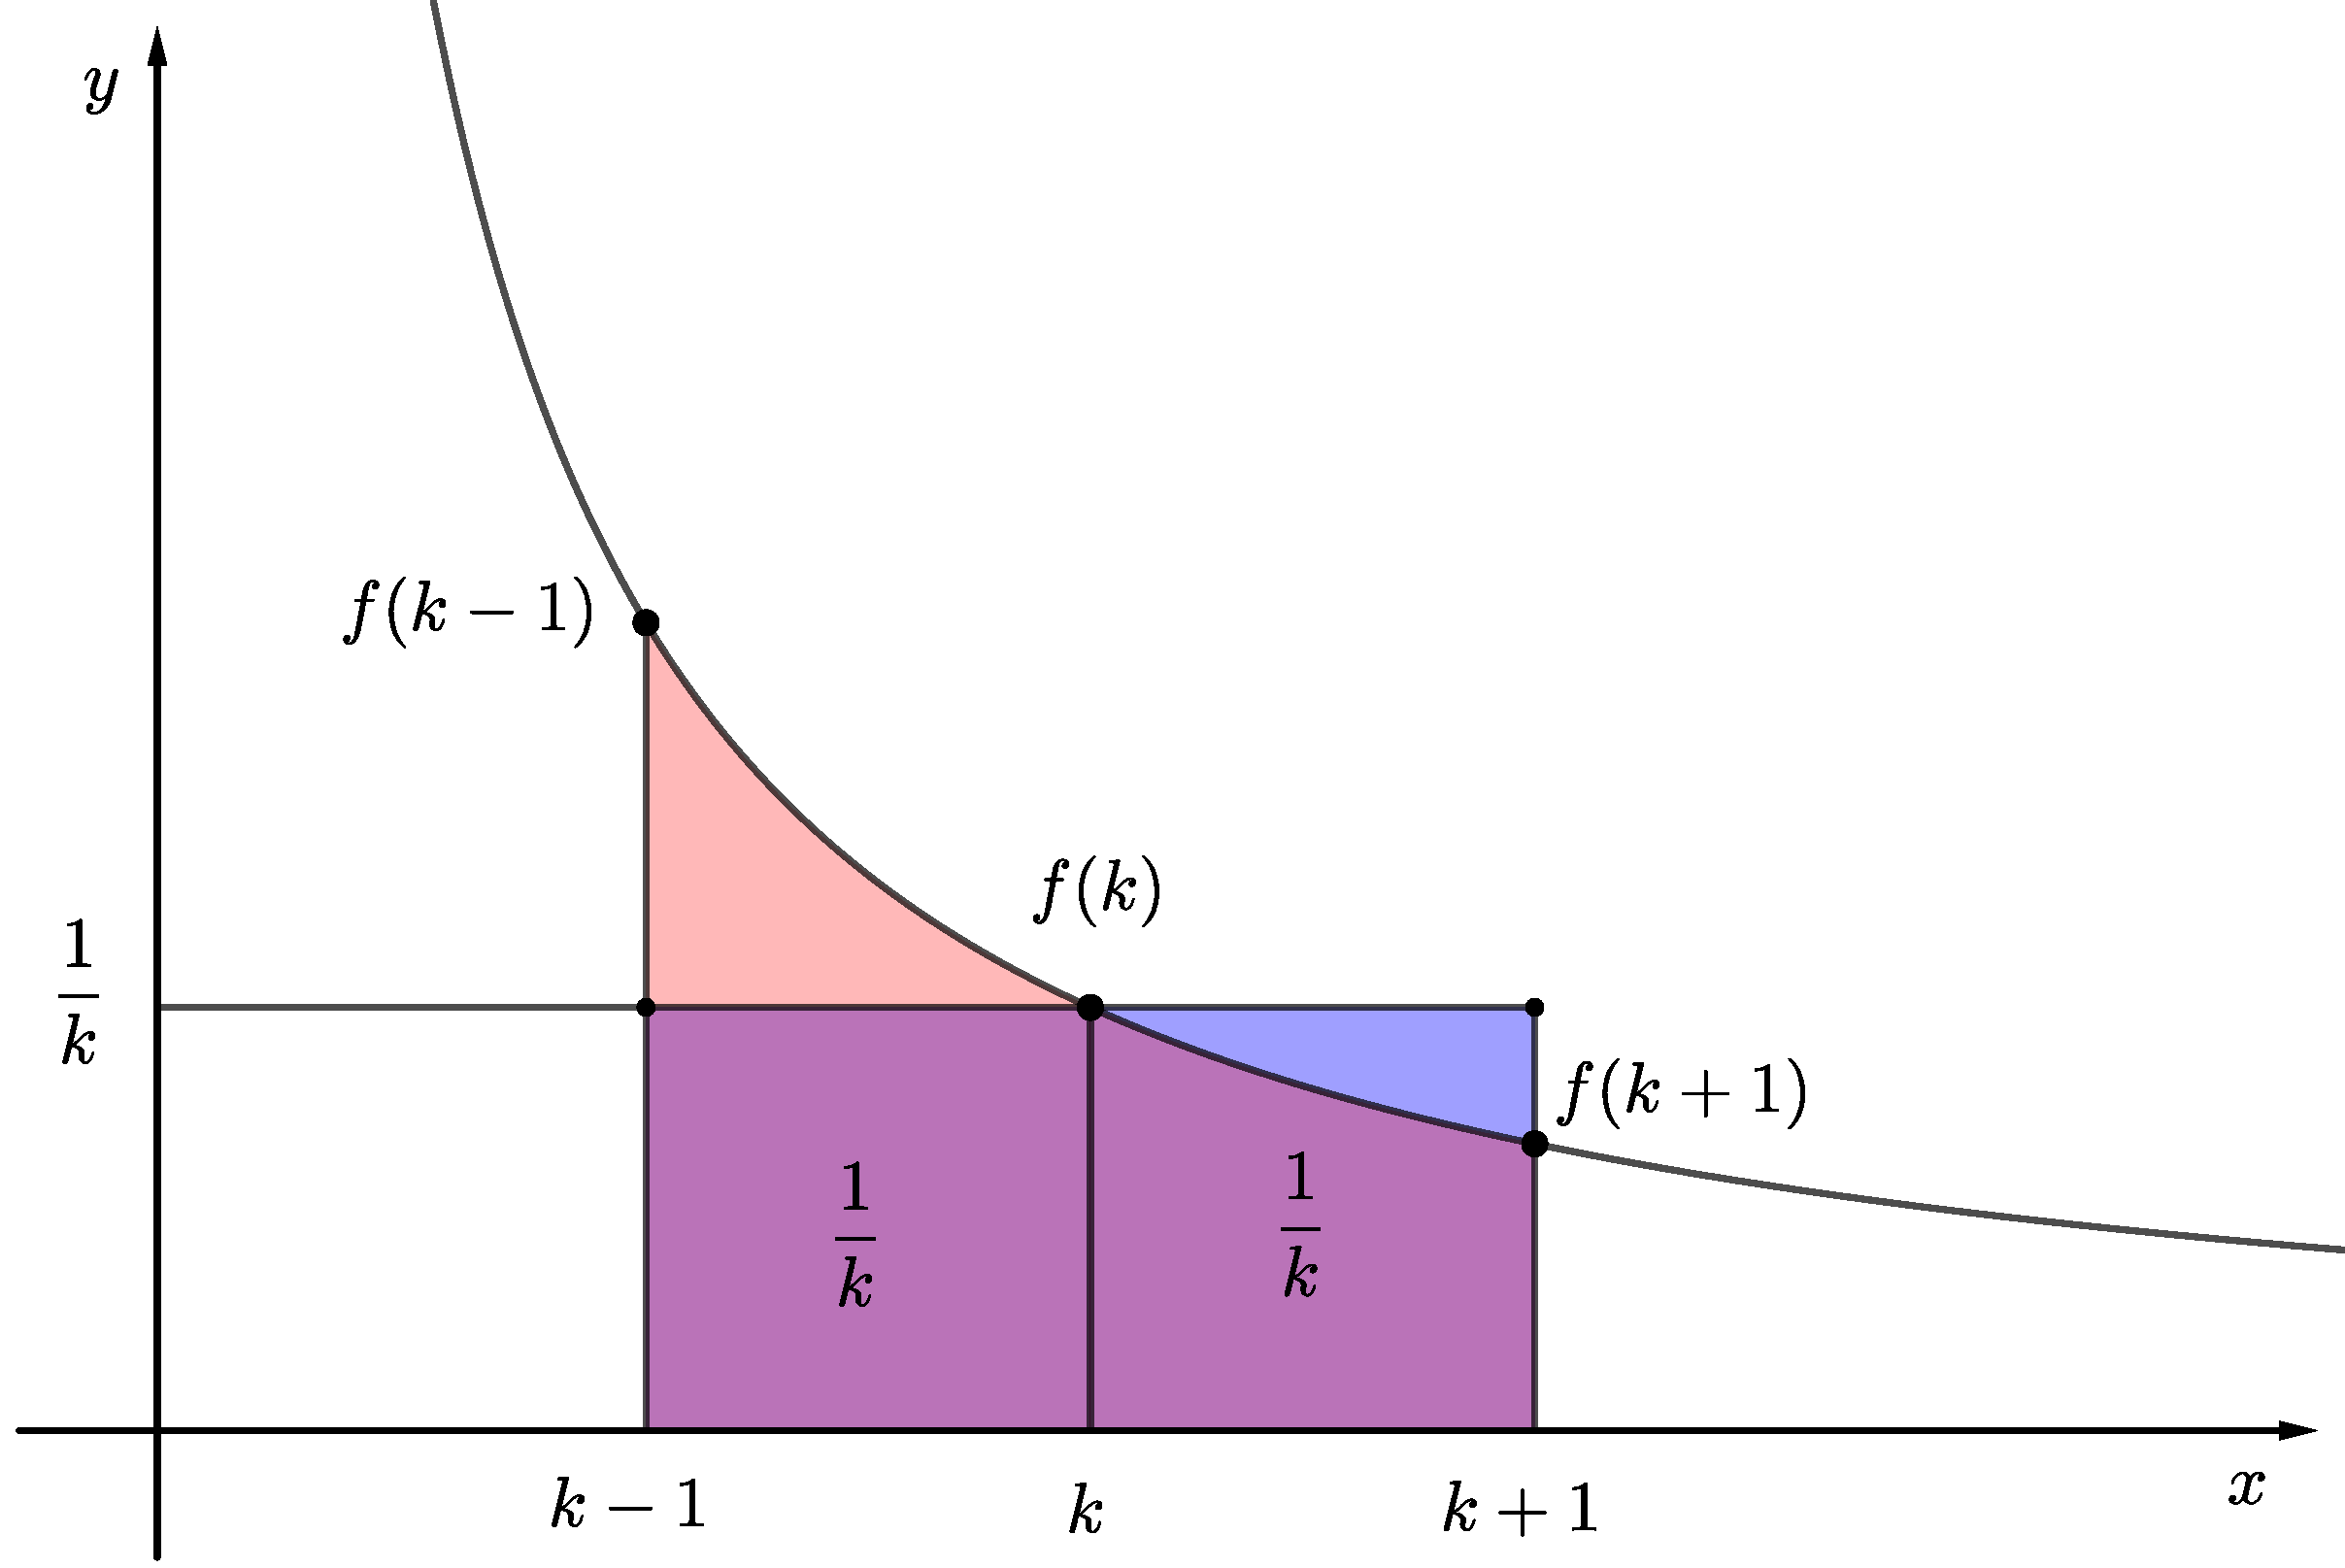
\includegraphics[width=0.7\textwidth]{grafici/intk}
	\caption{Approssimazione tramite integrale della somma della serie $\frac{1}{k}$.}
	\label{fig:intk}
\end{figure}
Da questa approssimazione si verifica che
\[
	\int_k^{k+1} \frac{dx}{x}\leq \frac{1}{k}\leq \int_{k-1}^k \frac{dx}{x}
\]
Estendendo l'approssimazione alla somma parziale:
\[
	\sum_{k=1}^n \int_k^{k+1} \frac{dx}{x}\leq \sum_{k=1}^n \frac{1}{k}\leq \sum_{k=1}^n \int_{k-1}^k \frac{dx}{x}
\]
Che applicando la proprietà \ref{int:somma} dell'integrale definito equivale a
\[
	\int_1^{n+1}\frac{dx}{x}\leq \sum_{k=1}^n \frac{1}{k} \leq \int_0^n\frac{dx}{x}
\]
Dalla prima disequazione si deduce che la somma parziale diverge, infatti:
\[
	\int_1^{n+1}\frac{dx}{x}=[\ln x]_1^{n+1}=\ln (n+1)\to+\infty
\]
Tuttavia, così com'è scritta la seconta disequazione non porta a nulla, dal momento che l'integrale improprio
\[
	\int_0^n\frac{dx}{x}=+\infty
\]
diverge in $0$ (infatti implica l'affermazione ovvia che la somma parziale sia minore di $+\infty$). È possibile però migliorare la stima: invece che stimare l'intero intervallo $(0,n)$ tramite l'integrale si utilizza per il primo valore della somma il valore stesso e per i successivi l'integrale:
\begin{align*}
	\sum_{k=1}^n \frac{1}{k} & \leq \sum_{k=1}^1 \frac{1}{k}+\int_1^n\frac{dx}{x} \\
	\sum_{k=1}^n \frac{1}{k} & \leq 1+\int_1^n\frac{dx}{x}
\end{align*}
Ovviamente, poiché come già dimostrato la somma parziale diverge anche la sua stima maggiore diverge:
\[
	1+\int_1^n\frac{dx}{x}=1+[\ln x]_1^n=1+\ln n
\]
Tuttavia, questo implica un'informazione ben più utile: poiché entrambi i valori di stima sono astintotici a $\ln n$, anche la somma parziale lo è:
\[
	\begin{cases}
		\ln(n+1)\sim \ln n \\
		1+\ln n\sim \ln n  \\
		\ln(n+1)\leq\sum_{k=1}^n \frac{1}{k}\leq 1+\ln n
	\end{cases}\Rightarrow
	\sum_{k=1}^n \frac{1}{k}\sim \ln n
\]

\begin{examp}
	Determinare il comportamento asintotico della seguente successione
	\[
		\ln(n!)
	\]
	La successione può essere espressa tramite una somma:
	\[
		\ln(n!)=\sum_{k=1}^n \ln k=\sum_{k=1}^n \ln k
	\]
	Questa somma può essere stimata tramite integrali della funzione $f(x)=\ln x$:
	\begin{gather*}
		\int_{k-1}^k \ln x ~dx\leq \ln k \leq \int_k^{k+1} \ln x ~dx\\
		\text{passando alle somme con $k=2$:}\\
		\int_1^n \ln x ~dx\leq \ln(n!) \leq \int_2^{n+1} \ln x ~dx
	\end{gather*}
	La primitiva di $f(x)$ è
	\[
		\int \ln x ~dx=x\ln x -\int x ~d(\ln x)=x\ln x -\int dx=x\ln x -x +c
	\]
	Quindi:
	\[
		n \ln n -n+1 \leq \ln(n!) \leq (n+1)\ln(n+1)-(n+1)-2\ln 2+2
	\]
	Entrambi i membri esterni sono astintotici a $n\ln n$, pertanto lo sarà anche la successione $\ln(n!)$.
\end{examp}

\begin{examp}
	Calcolare il limite di
	\[
		c_n=\sum_{k=n}^{2n} \frac{1}{k}
	\]
	Stimando tramite integrali ($f(x)=\frac{1}{k}$):
	\begin{gather*}
		\int_l^{k+1}\frac{dx}{x}\leq \frac{1}{k}\leq \int_{k-1}^k \frac{dx}{x}\\
		\int_n^{2n+1}\frac{dx}x \leq \sum_{n}^{2n} \frac{1}{k} \leq \int_{n-1}^{2n} \frac{dx}{x}\\
		\ln(2n+1)-\ln n \leq c_n \leq \ln(2n) -\ln(n-1)\\
		\ln\left(\frac{2n+1}{n}\right) \leq c_n \leq \ln\left(\frac{2n}{n-1}\right)
	\end{gather*}
	Essendo i membri esterni asintotici a $\ln 2$, il valore del limite è $\ln 2$.
\end{examp}

\begin{examp}
	Studiare il comportamento di
	\[
		\sum_{k=1}^{+\infty} ke^{-k}
	\]
	La serie si può stimare tramite integrali, tuttavia la funzione $f(x)=xe^{-x}$ non è elementare. Studiando la derivata $f'(x)=e^{-x}(1-x)$ si trova un unico massimo assoluto in $x=1$, dopo il quale la funzione decresce. Poiché per la stima integrale è necessaria una funzione monotona, si sceglie di partire da $k=2$, in modo che i rettangoli di base unitaria (si veda la figura \ref{fig:intk} riguardante però un'altra funzione non si estendano per $x<1$. Dal momento che la somma ha valori finiti per $k<2$ (uno), è possibile aggiungere tali valori "manualmente" dopo la stima. Per $k\geq2$ si ottiene:
	\begin{gather*}
		\int_k^{k+1} f(x)~dx \leq ke^{-k} \leq int_{k-1}^k f(x)~dx\\
		\int_2^{n+1} f(x)~dx \leq \sum_{k=2}^n ke^{-k} \leq \int_1^n f(x)~dx
	\end{gather*}
	L'integrale di $f(x)$ è
	\[
		\int xe^{-x}~dx=-\int x~d(e^{-x})=-xe^{-x}+\int e^{-x}~dx=-xe^{-x}-e^{-x}+c
	\]
	Tornando a $k\geq1$ e aggiungendo il valore della somma per $k=1$, ovvero $\frac{1}{e}$:
	\[
		\frac{1}{e}+\frac{3}{e^2} \leq \sum_{k=2}^n ke^{-k} \leq \frac{3}{e}
	\]
	Questa è una stima del valore della somma, che quindi converge. Per quanto riguarda lo studio del resto:
	\[
		\int_{n+1}^{+\infty} f(x)~dx \leq \sum_{k=2}^{+\infty} ke^{-k} \leq \int_n^{+\infty} f(x)~dx
	\]
	Svolgendo gli integrali impropri si ottiene:
	\[
		(n+2)e^{-(n+1)} \leq \sum_{k=2}^{+\infty} ke^{-k} \leq (n+1)e^{-n}
	\]
	Vale:
	\begin{gather*}
		(n+2)e^{-(n+1)}\sim ne^{-(n+1)}=\Theta(ne^{-n})\\
		(n+1)e^{-n}\sim ne^{-n}=\Theta(ne^{-n})
	\end{gather*}
	Quindi il resto è $\Theta(ne^{-n})$.
\end{examp}


\subsection{Proprietà delle somme finite nelle serie}
È innanzitutto utile menzionare la seguente proprietà
\begin{teor}[Condizione necessaria di convergenza]
	\label{teor:necconv}
	\[
		\sum_{k=0}^{+\infty} a_k\quad\text{converge}\quad\Rightarrow\quad a_k\to0\qquad k\to+\infty
	\]
\end{teor}
\begin{proof}
	\[
		\sum_{k=0}^n a_k-\sum_{k=0}^{n-1} a_k=a_n
	\]
	Le due somme non sono altro che successioni $S_n$ e $S_{n-1}$. Se per ipotesi $S_n\to S\in\R$, allora, per la proprietà delle successioni \vref{suc:trasl}, vale $S_{n-1}\to S$. La differenza di queste, cioè $a_n$, tende quindi a $0$.
\end{proof}

È naturale chiedersi se le proprietà applicate alle somme finite valgano anche per le serie infinite. La prima che è utile discutere è quella delle somme telescopiche (paragrafo \ref{sum:tele}). È possibile infatti applicare la proprietà alle somme parziali:
\[
	\sum_{k=1}^n a_k=\sum_{k=1}^n(b_k-b_{k+1})=b_1-b_{n+1}\to b_1-b_\infty
\]
Il limite della somma parziale, pertanto, esiste se
\[
	\exists \lim_{n\to+\infty} b_k := b_\infty
\]

Un'altra proprietà di cui ha senso questionare la validità è
\[
	\sum_{k=0}^{+\infty} a_k+b_k=\sum_{k=0}^{+\infty} a_k+\sum_{k=0}^{+\infty} b_k
\]
Da cui deriverebbe
\[
	\sum_{k=0}^{+\infty} c*a_k=c\sum_{k=0}^{+\infty} a_k
\]
Anche in questo caso ci si riconduce tramite la definizione alle somme parziali:
\[
	\sum_{k=0}^n (a_k+b_k)=\sum_{k=0}^n a_k + \sum_{k=0}^n b_k
\]
Posto che la prima somma sia regolare:
\[
	\exists \lim_{n\to+\infty} \sum_{k=0}^n a_k=a\qquad\land\qquad\exists \lim_{n\to+\infty} \sum_{k=0}^n b_k=b
\]
Che implica
\[
	\exists \lim_{n\to+\infty} \sum_{k=0}^n (a_k+b_k)=a+b
\]
A patto che i due limiti non siano infiniti discordi, nel qual caso si otterrebbe una forma di indecisione.


\subsection{Serie a termini definitivamente uguali}
\begin{teor}
	\label{ser:defugu}
	Se date due successioni $a_n$ e $b_n$ vale $a_n=b_n$ definitivamente, allora le relative somme infinite
	\[
		A=\sum_{n=0}^{+\infty} a_n, B=\sum_{n=0}^{+\infty} b_n
	\]
	hanno lo stesso carattere e la stessa velocità di convergenza/divergenza.
\end{teor}
\begin{proof}
	Per ipotesi:
	\[
		\exists\nu\mid a_n=b_n\forall n\geq\nu
	\]
	Dovendo calcolare il limite delle somme parziali per $n\to+\infty$, è lecito applicare ipotesi sulla grandezza arbitraria di $n$: in particolare, si pone $n\geq\nu$:
	\[
		A_n-A_{\nu-1}=\sum_{k=\nu}^n a_k=\sum_{k=\nu}^n b_k=B_n-B_{\nu-1}
	\]
	Da ciò si ricava che
	\[
		A_n=(A_{\nu-1}-B_{\nu-1})+B_n
	\]
	Ovvero, $A_n$ e $B_n$ differiscono di una costante $c_\nu$ dipendente solo da $\nu$. Questo significa che
	\[
		\lim_{n\to+\infty} A_n=c_\nu+\lim_{n\to+\infty} B_n
	\]
	Quindi:
	\begin{gather}
		A_n\to+\infty\Rightarrow B_n\to+\infty\land A_n\sim B_n\\
		A_n\to A\in\R\Rightarrow B_n\to B\in\R\land A_n\sim B_n
	\end{gather}
	E viceversa. Per quanto riguarda i resti, nel caso di convergenza:
	\[
		A-A_n=\sum_{k=n+1}^{+\infty} a_k=\sum_{k=n+1}^{+\infty} b_k=B-B_n
	\]
	Scelto $n\geq\nu$.
\end{proof}
Una conseguenza di questo teorema è che somme di serie di stesse successioni ma diversi indici minimi hanno lo stesso comportamento.

\subsection{Serie a termini definitivamente positivi}
\begin{teor}
	\label{ser:defpos}
	Se $a_k\geq0$ definitivamente, allora
	\[
		\sum_{k=0}^{+\infty} a_k
	\]
	è regolare.
\end{teor}
\begin{proof}
	La ridotta
	\[
		A_n=\sum_{k=0}^n a_k
	\]
	è definitivamente monotona crescente, infatti vale $A_{n+1}\geq A_n$ definitivamente poiché vale $A_{n+1}-A_n=a_{n+1}\geq 0$ definitivamente. Da ciò deriva che $A_n\to\text{sup}\{A_k\mid k\in\N\}$ (teorema \vref{suc:rego}), quindi la somma della serie esiste.
\end{proof}

\subsection{Criterio del confronto}
\begin{teor}[del confronto per le serie]
	\label{ser:confr}
	Date due successioni $a_k$ e $b_k$ a termini definitivamente positivi tali che $a_k\leq b_k$ definitivamente, se la serie che ha per termini le immagini di $b_k$ converge allora la serie che ha per termini le immagini di $a_k$ converge; se la seconda diverge allora la prima diverge. In simboli:
	\begin{gather*}
		\exists\nu\mid 0\leq a_k\leq b_k \quad\forall k\geq\nu\\
		\sum_{k=0}^{+\infty} a_k \text{ diverge}\quad\Rightarrow\quad \sum_{k=0}^{+\infty} b_k \text{ diverge}\\
		\sum_{k=0}^{+\infty} b_k \text{ converge}\quad\Rightarrow\quad \sum_{k=0}^{+\infty} a_k \text{ converge}
	\end{gather*}
\end{teor}
\begin{proof}
	Per $n\geq\nu$ (quindi opportunamente grande):
	\[
		\tilde A_n=\sum_{k=\nu}^n a_k\leq \tilde B_n=\sum_{k=\nu}^n b_k
	\]
	Se $\tilde A_n$ diverge si ha definitivamente
	\[
		M<\tilde A_n<\tilde B_n\qquad\forall M
	\]
	quindi $\tilde B_n$ è regolare e diverge. Essendo a termini definitivamente positivi, $\tilde A_n$ è regolare (teorema \ref{ser:defpos}). Se $\tilde B_n$ converge allora è limitata, quindi:
	\[
		\exists m \mid \tilde A_n \leq \tilde B_n\leq m
	\]
	Essendo $A_n$ limitata allora converge. Inoltre, essendo tali somme delle successioni, vale, per il teorema \vref{suc:glelandau}:
	\begin{equation}
		\tilde A_n =O(\tilde B_n)\quad\land\quad\tilde B_n =\Omega(\tilde A_n)
	\end{equation}
	e, nel caso di convergenza:
	\begin{equation}
		B-\tilde B_n=\Omega(A-\tilde A_n)\quad\land\quad\tilde A-A_n=O(B-\tilde B_n)
	\end{equation}

	Poiché definitivamente vale
	\[
		A_n=\sum_{k=0}^n a_k=\tilde A_n=\sum_{k=\nu}^n a_k\land B_n=\sum_{k=0}^n b_k=\tilde B_n=\sum_{k=\nu}^n b_k
	\]
	allora per il teorema \ref{ser:defugu} il comportamento delle somme iniziali è lo stesso.
\end{proof}
\begin{corol}
	\label{ser:confrasin}
	Date le serie degli $a_n$ e dei $b_n$ tali che $a_n,b_n\geq0$ definitivamente, vale
	\[
		a_n\sim b_n\quad\Rightarrow\quad \sum_{k=0}^n a_n=\Theta\sum_{k=0}^n b_n
	\]
	E le serie hanno, ovviamente, lo stesso carattere.
\end{corol}
\begin{proof}
	Poiché $\frac{b_n}{a_n}\to1$, si ha definitivamente:
	\[
		\frac{a_n}{2}\leq b_n\leq 2a_n
	\]
	Dal momento che le serie degli $\frac{a_n}{2}$ e dei $2a_n$ sono l'una $\Theta$ dell'altra, per il teorema \ref{ser:confr} la tesi è vera. Dimostrazione analoga occorre nel caso che come ipotesi si abbia $a_n=\Theta(b_n)$
\end{proof}

\begin{examp}
	Studiare la serie
	\[
		\sum_{k=1}^{+\infty}[1+2(k-\sqrt{k+k^2})]
	\]
	Sviluppando la radice con lo sviluppo notevole:
	\begin{gather*}
		1+2k\left(1-1-\frac{1}{2k}+\frac{1}{8k^2}+o\left(\frac{1}{k^2}\right)\right)=\\
		=1-1+\frac{1}{4k}+o\left(\frac{1}{k}\right)\sim\frac{1}{4k}=\Theta\left(\frac{1}{k}\right)
	\end{gather*}
	La serie diverge come $\ln n$ (serie armonica).
\end{examp}

\begin{examp}
	\[
		\sum_{k=2}^{+\infty}\frac{1}{(\ln k)^8}
	\]
	La serie è regolare dal momento che i suoi termini sono positivi. Inoltre, definitivamente vale:
	\begin{gather}
		\label{eq:serex1}
		1\leq(\ln k)^8\leq k\\
		\frac{1}{k}\leq\frac{1}{(\ln k)^8}\leq 1\notag
	\end{gather}
	Dalla la prima disequazione si deduce che la serie diverge. Per le somme parziali, applicando il teorema \ref{ser:confr}, vale inoltre:
	\[
		A_n=\Omega\left(\sum_{k=0}^n \frac{1}{k}\right)=\Omega(\ln n) \quad\land\quad A_n=O\left(\sum_{k=0}^n 1\right)=O(n)\\
	\]
	Volendo migliorare questa stima, si può notare che la seconda equazione della \ref{eq:serex1} vale anche per $k^\varepsilon$, $\forall\varepsilon>0$, da cui:
	\[
		A_n=\Omega(\ln n)\cap O(n^\varepsilon)
	\]
\end{examp}


\subsection{Convergenza assoluta}
\begin{defin}
	Si dice che una serie che ha per termini le immagini di una successione $a_n$ converge assolutamente se la serie che ha per termini le immagini di $\abs{a_n}$ converge:
	\[
		\sum_{k=m}^{+\infty} \abs{a_n}\to A\in\R
	\]
\end{defin}
\begin{teor}
	\label{teor:convass}
	Se una serie converge assolutamente, allora converge.
	\[
		\sum_{n=1}^{+\infty}\abs{a_n}\to A'\in\R\quad\Rightarrow\quad \sum_{n=1}^{+\infty} a_n\to A\in\R
	\]
\end{teor}
\begin{proof}
	Per ogni $a_n$ vale:
	\[
		-\abs{a_n}\leq a_n\leq \abs{a_n}
	\]
	Aggiungendo $a_n$ a tutti i membri
	\begin{gather*}
		\abs{a_n}-\abs{a_n}\leq a_n+\abs{a_n}\leq \abs{a_n}+\abs{a_n}\\
		0\leq a_n+\abs{a_n}\leq 2\abs{a_n}
	\end{gather*}
	Chiamando $b_n$ il membro centrale della relazione, si verifica che la serie che ha per termini le immagini di tale successione è convergente, dal momento che $b_n$ è maggiore di $0$ (da cui la regolarità) e minore di $2\abs{a_n}$, convergente per ipotesi. Dal momento che vale la relazione
	\[
		a_n\leq b_n-\abs{a_n}
	\]
	e le serie che hanno per argomento le due successioni al secondo membro convergono, allora anche $a_n$ converge.
\end{proof}


\subsection{Criteri della radice e del rapporto}
\begin{teor}
	Data una serie che ha per termini le immagini di una successione $a_n$ definitivamente non negativa, posto, se esiste:
	\begin{gather*}
		\sqrt[k]{a_k}\to L\\
		\frac{a_{k+1}}{a_k}\to L
	\end{gather*}
	\begin{itemize}
		\item Se $0\leq L<1$ allora la serie converge
		\item Se $L>1$ allora la serie diverge
	\end{itemize}
\end{teor}
\begin{proof}
	Si dimostra il criterio della radice. È possibile dimostrare il criterio del rapporto e che i due limiti $L$ sono uguali.

	In analogia con la dimostrazione del criterio della radice per le successioni (\vref{teor:sucradice}), per ogni coppia di estremi $p<q$ di un intorno di $L$ vale, definitivamente:
	\begin{gather}
		p<\sqrt[k]{a_k}<q\quad\Rightarrow\quad p^k<a_k<q^k\notag\\
		\label{eq:radiceserie}
		\sum_k^{+\infty}p^k<\sum_k^{+\infty}a_k<\sum_k^{+\infty}q^k
	\end{gather}
	\begin{itemize}
		\item Nel caso di $0\leq L<1$ è possibile scegliere un $q<1$. La serie dei $q^k$ sarà quindi una serie geometrica di ragione minore di $1$, pertanto converge. Per il teorema \ref{ser:confr} del confronto la serie degli $a_k$ converge;
		\item Nel caso di $L>1$ si ha $a_k>1$ definitivamente. Poiché la serie degli $a_k$ è regolare (essendo a termini definitivamente positivi) ma non soddisfa la condizione necessaria di convergenza (teorema \ref{teor:necconv}), la serie diverge.
	\end{itemize}
	In aggiunta alle conclusioni è possibile dire, per il teorema del confronto applicato alle serie della \ref{eq:radiceserie}, che
	\begin{itemize}
		\item Se la serie degli $a_k$ diverge:
		      \begin{gather*}
			      \sum^n a_k=\Omega\left(\sum^n p^k\right)\quad\land\quad \sum^n a_k=O\left(\sum^n q^k\right)\\
			      \sum^n p^k=\Theta(p^n)\quad\land\quad \sum^n q^k=\Theta(q^n)\\
			      \sum^n a_k=\Omega(p^n)\cap O(q^n) \qquad \forall(p<L<q)
		      \end{gather*}
		\item Se la serie degli $a_k$ converge, essendo
		      \[
			      R_n=S-\sum^n a_k=\Theta\left(\sum^n a_k\right)
		      \]
		      valgono le stesse considerazioni del caso precedente per $R_n$.
	\end{itemize}
\end{proof}
\begin{examp}
	\[
		\sum_{k=1}^{+\infty} \frac{k^2+2^k}{\ln k +\sqrt k}
	\]
	Vale
	\[
		a_k=\frac{k^2+2^k}{\ln k +\sqrt k}\sim \frac{2^k}{\sqrt k}=b_k
	\]
	Essendo la successione divergente, anche la serie lo è. Ai fini di studiare l'andamento, si applica il criterio del rapporto:
	\[
		\frac{b_{k+1}}{b_k}=\frac{2^{k+1}}{\sqrt{k+1}}*\frac{\sqrt k}{2^k}\to 2<1
	\]
	Da cui
	\[
		\sum_{k=0}^n b_k=\Omega(p^n)\cap O(q^n)
	\]
	Inoltre
	\[
		\frac{2^k}{\sqrt k}\leq 2^n\quad\Rightarrow\quad \sum_{k=0}^n b_k=\Omega(p^n)\cap O(2^n)
	\]
	Dal momento che, per il teorema \ref{ser:confrasin}, la somma parziale degli $a_k$ è $\Theta$ della somma parziale dei $b_k$, vi vale la stessa relazione, infatti:
	\[
		\sum_{k=0}^n a_k = \Theta\left(\sum_{k=1}^n\right)=
		\begin{cases}
			\Theta(\Omega(p^n))=\Omega(p^n) \\
			\Theta(O(2^n))=O(2^n)
		\end{cases}
	\]
\end{examp}

%% Copyright (C) 2019-2021 Alessandro Clerici Lorenzini
%
% This work may be distributed and/or modified under the
% conditions of the LaTeX Project Public License, either version 1.3
% of this license or (at your option) any later version.
% The latest version of this license is in
%   http://www.latex-project.org/lppl.txt
% and version 1.3 or later is part of all distributions of LaTeX
% version 2005/12/01 or later.
%
% This work has the LPPL maintenance status `maintained'.
%
% The Current Maintainer of this work is Alessandro Clerici Lorenzini
%
% This work consists of the files listed in work.txt


\section{Serie di potenze}
\begin{defin}
	Si definisce serie di potenze di centro zero\footnote{Una serie di potenze può avere centro diverso da zero. Una serie di potenze di centro $x_0$ si presenta nella forma:
		\[
			\sum_{k=0}^{+\infty} a_n (x-x_0)^n
		\]} una serie nella forma:
	\[
		A(x)=\sum_{n=0}^{+\infty} a_n x^n
	\]
	Con $a_n\in\R\forall n\land x\in\R$
\end{defin}
Per studiare il comportamento di una serie di potenze è innanzitutto utile fare un'osservazione:
\[
	A(0)=\sum_{n=0}^{+\infty} a_n*0^n=
	\begin{cases}
		a_0\quad & n=0    \\
		0 \quad  & n\neq0
	\end{cases}\Rightarrow A(0)\to a_0
\]
In questo caso si sceglie $0^0=1$ per convenzione.

È notevole altresì sottolineare che la serie geometrica è un caso particolare di serie di potenze, con $a_n=1$ costante.

\subsubsection{Raggio di convergenza}
Per studiare la convergenza di una serie di potenze, si studia la convergenza assoluta, dal momento che per il teorema \ref{teor:convass} essa implica la convergenza.
\[
	\sum_{n=0}^{+\infty}\abs{a_n*x^n}=\sum_{n=0}^{+\infty}\abs{a_n}\abs{x}^n
\]
Si applica poi un criterio come quelli del rapporto e della radice:
\[
	\begin{array}{cc}
		\text{Rapporto}                                                                                                 & \text{Radice}                                                            \\[1ex]
		\dfrac{\abs{a_{n+1}}\abs{x}^{n+1}}{\abs{a_n}\abs{x}^n}=\dfrac{\abs{a_{n+1}}}{\abs{a_n}}\abs{x}\to L\abs{x}\quad & \quad\sqrt[n]{\abs{a_n}\abs{x}^n}=\sqrt[n]{\abs{a_n}}\abs{x}\to L\abs{x}
	\end{array}
\]
Quindi, posto che $L$ esista:
\begin{itemize}
	\item Per $L\abs{x}<1\Rightarrow \abs{x}<\frac{1}{L}$ la serie converge assolutamente e quindi converge;
	\item Per $L\abs{x}>1\Rightarrow \abs{x}>\frac{1}{L}$ la serie diverge assolutamente e quindi quantomeno non converge
\end{itemize}
Il numero $\frac{1}{L}=R$ si chiama raggio di convergenza. Si può dimostrare che $A(R)$ non è definita e che, in particolare, $R$ è il minore, in modulo\footnote{Per la precisione, in generale, è il più vicino al centro.}, dei punti in cui $A(x)$ non è definita. Nelle serie geometriche, come è facile verificare, il raggio è $1$.

Quando $L=0$, $R$ non è definito, tuttavia si verifica la prima delle due situazioni sopracitate, quindi la serie converge per ogni $x$. Si dice che $R=+\infty$. Quando $L=+\infty$, $R$ non è definito, tuttavia si verifica la seconda situazione, ad eccezione di $x=0$, nel qual caso la serie converge. Si dice che $R=0$, o che la serie è formale.

\subsubsection{Polinomi tramite serie di potenze}
Un polinomio può essere scritto tramite una serie di potenze, per esempio:
\begin{examp}
	\begin{gather*}
		\sum_{n=0}^{+\infty} a_n x^n= x-\sqrt2 x^3 + 5x^4\\
		\text{con }a_n=
		\begin{cases}
			1\qquad       & n=1           \\
			-\sqrt2\qquad & n=3           \\
			5\qquad       & n=4           \\
			0\qquad       & 1<n<3\lor n>4
		\end{cases}
	\end{gather*}
	In questo caso si ha $R=+\infty$.
\end{examp}


\subsection{Combinazione lineare}
\begin{defin}[combinazione lineare di serie di potenze]
	\label{ser:comblin}
	\begin{equation}
		A\sum_{n=0}^{+\infty}a_n x^n+B\sum_{n=0}^{+\infty} b_nx^n=\sum_{n=0}^{+\infty} (Aa_k+Bb_k)x^n
	\end{equation}
	Da cui deriva
	\begin{equation}
		\label{eq:cperserie}
		c*\sum_{n=0}^{+\infty} a_nx^n=\sum_{n=0}^{+\infty}ca_nx^n
	\end{equation}
\end{defin}
L'operazione ha come elemento neutro la serie nulla e come inverso la serie opposta. Inoltre, per $A=B=1$, se la prima serie ha raggio di convergenza $R_A$ e la seconda $R_B$, ci si aspetta che il raggio di convergenza della loro combinazione lineare sia non inferiore a $\text{min}\{R_A,R_B\}$, e che in caso di convergenza la somma della combinazione sia uguale alla somma delle somme delle due serie. Entrambi questi risultati vengono chiaramente influenzati (ma in modo coerente) se i coefficienti sono diversi da $1$.

\begin{examp}
	Calcolare il raggio di convergenza di
	\[
		\sum_{n=0}^{+\infty}(2^{n+1}+1)x^n=
	\]
	La serie è una combinazione lineare, quindi:
	\[
		=2\sum_{n=0}^{+\infty}2^nx^n+\sum_{n=0}^{+\infty}x^n
	\]
	È possibile applicare una sostituzione, dal momento che $2^nx^n=(2x)^n$ e $t=2x$ non dipende da $n$:
	\[
		=2\sum_{n=0}^{+\infty}t^n+\sum_{n=0}^{+\infty}x^n
	\]
	La prima delle due serie converge a $\frac{1}{1-t}=\frac{1}{1-2x}$ con raggio $\frac{1}{2}$, mentre la seconda converge a $\frac{1}{1-x}$ con raggio $1$. La combinazione lineare, nonché serie iniziale, converge quindi a
	\[
		\frac{1}{1-2x}+\frac{1}{1-x}
	\]
	con raggio $\abs{x}<\frac{1}{2}$.
\end{examp}


\subsection{Derivazione}
La derivata di una serie di potenze viene così definita:
\begin{defin}
	\[
		D\left(\sum_{n=0}^{+\infty} a_nx^n\right):=\sum_{n=0}^{+\infty}(n+1)a_{n+1}x^n
	\]
\end{defin}
La definizione è coerente con il concetto di derivata, infatti:
\[
	D(a_0+a_1x+a_2x^2+a_3x^3+\dots)=0+a_1+a_2x+a_3x^2+\dots
\]
Vale inoltre la seguente relazione, che non dimostriamo:
\[
	D\left(\sum_{n=0}^{+\infty} a_nx^n\right)=\sum_{n=0}^{+\infty}D(a_nx^n)=\sum_{n=0}^{+\infty}a_nnx^{n-1}
\]
di cui l'ultima espressione è equivalente alla definizione, in quanto per $n=0$ il coefficiente di $x^{-1}$ è $0$.

\subsubsection{Somma e raggio della derivata}
Per quanto riguarda la somma della derivata, si dimostra che:
\begin{teor}
	Se una serie di potenze di raggio $R$ converge ad $A(x)$, allora la sua derivata converge ad $A'(x)$:
	\[
		\sum_{n=0}^{+\infty} a_n x^3=A(x)\Rightarrow\sum_{n=0}^{+\infty} a_n 2x^2=A'(x)\qquad\forall x\in(-R,R)
	\]
	Con $R$ comune.
\end{teor}
Benché la dimostrazione vada oltre gli strumenti precedentemente introdotti, si dimostra in seguito l'uguaglianza dei raggi:
\begin{proof}
	Applicando il criterio del rapporto all'argomento della derivata:
	\[
		\frac{1}{R'}=\lim_{n\to+\infty}\frac{b_{n+1}}{b_n}=\lim_{n\to+\infty}\frac{n+2}{n+1}*\frac{a_{n+2}}{a_{n+1}}=\frac{1}{R}
	\]
	Nell'ultimo prodotto, il primo fattore tende a $1$, mentre il secondo è il criterio del rapporto applicato alla serie non derivata e traslato di $+1$: tende pertanto allo stesso limite, cioè $\frac{1}{R}$.
\end{proof}

\begin{examp}
	\label{ex:dergeom}
	Calcolare la somma della seguente serie di potenze:
	\[
		\sum_{n=0}^{+\infty}(n+1)x^n=D\left(\sum_{n=0}^{+\infty}x^n\right)=D\left(\frac{1}{1-x}\right)=\frac{1}{(1-x)^2}
	\]
\end{examp}

\subsubsection{Derivata $m$-esima}
Calcolare le derivate successive alla prima significa calcolare la derivata di una derivata. Ad esempio:
\begin{examp}
	\[
		D^2\left(\sum_{n=0}^{+\infty}a_nx^n\right)=D\left(D\left(\sum_{n=0}^{+\infty}a_nx^n\right)\right)=D\left(\sum_{n=0}^{+\infty}(n+1)a_{n+1}x^n\right)
	\]
	Chiamando il coefficiente di $x^n$ $b_n$:
	\[
		=\sum_{n=0}^{+\infty}(n+1)b_{n+1}x^n=\sum_{n=0}^{+\infty}(n+1)(n+2)a_{n+2}x^n
	\]
\end{examp}

La derivata $m$-esima di una serie di potenze è espressa dalla seguente formula generalizzata:
\begin{equation}
	D^m\left(\sum_{n=0}^{+\infty}a_nx^n\right)=\sum_{n=0}^{+\infty}(n+1)(n+2)\dots(n+m)a_{n+m}x^n
\end{equation}
Questa scrittura viene compattata con il coefficiente binomiale, dividendo entrambi i membri per $m!$:
\[
	\frac{1}{m!}D^m\left(\sum_{n=0}^{+\infty}a_nx^n\right)=\sum_{n=0}^{+\infty}\binom{n+m}{m}a_{n+m}x^n
\]

Applicando la formula alla serie geometrica di potenze vale:
\[
	\frac{1}{(1-x)^{m+1}}=\frac{1}{m!}D^m\left(\sum_{n=0}^{+\infty}x^n\right)=\sum_{n=0}^{+\infty}\binom{n+m}{m}x^n
\]
Dove il primo membro è la derivata $m$-esima della somma divisa per $m!$.


\subsection{Prodotto di Cauchy}
Il prodotto di Cauchy (o di convoluzione) si pone lo scopo di definire il prodotto di due serie.
\[
	\left(\sum_{n=0}^{+\infty} a_nx^n\right)\left(\sum_{n=0}^{+\infty}b_nx^n\right)=\sum_{n=0}^{+\infty}\left(\sum_{k=0}^na_kb_{n-k}\right)x^n
\]
Infatti, in modo esplicito:
\[
	(a_0+a_1x+a_2x^2+a_3x^3+\dots)(b_0+b_1x+b_2x^2+b_3x^3+\dots)
\]
Ai termini di $n$-esimo grado contribuiscono solo i coefficienti la cui somma è $n$:
\[
	a_0b_0+(a_0b_1+a_1b_0)x+(a_0b_2+a_1b_1+a_2b_0)x^2+\dots
\]
da cui l'espressione di cui sopra.

Vale inoltre il seguente teorema
\begin{teor}
	Il prodotto di Cauchy di due serie convergenti converge al prodotto delle somme:
	\[
		\begin{cases}
			\displaystyle\sum_{n=0}^{+\infty}a_nx^n=A(x)\quad\text{per }\abs{x}<R_A \\[2ex]
			\displaystyle\sum_{n=0}^{+\infty}b_nx^n=B(x)\quad\text{per }\abs{x}<R_B
		\end{cases}\Rightarrow
		\sum_{n=0}^{+\infty}\left(\sum_{k=0}^na_kb_{n-k}\right)x^n=A(x)B(x)
	\]
	con raggio $\abs{x}<\text{min}\{R_A,R_B\}$
\end{teor}
\begin{examp}
	\[
		\left(\sum_{n=0}^{+\infty}x^n\right)^2=\sum_{n=0}^{+\infty}\left(\sum_{k=0}^n 1*1\right)x^n=\sum_{n=0}^{+\infty}(n+1)x^n
	\]
	Che come già visto all'esempio \ref{ex:dergeom} non è altro che la derivata della serie geometrica ed è quindi uguale a $\frac{1}{(1-x)^2}$.
\end{examp}

\begin{examp}
	\begin{equation}
		\label{ex:prodcauchy}
		x^p\sum_{n=0}^{+\infty}a_nx^n=\sum_{n=0}^{+\infty}a_nx^{n+p}=\sum_{n=p}^{+\infty}a_{n-p}x^n
	\end{equation}
	In questa soluzione il prodotto è stato interpretato come una combinazione lineare di una costante con una successione (\ref{eq:cperserie} alla definizione \ref{ser:comblin}). Il prodotto può essere interpretato anche come il prodotto di Cauchy della serie di potenze di $a_n$ con la serie:
	\[
		\sum_{n=0}^{+\infty}\delta_{np}x^n\qquad\text{con }\delta_{np}=
		\begin{cases}
			1\quad & n=p     \\
			0\quad & n\neq p
		\end{cases}
	\]
	In tal caso il prodotto equivale a
	\[
		\left(\sum_{n=0}^{+\infty}\delta_{np}x^n\right)\left(\sum_{n=0}^{+\infty}a_nx^n\right)=\sum_{n=0}^{+\infty}\left(\sum_{k=0}^n \delta_{kp}a_{n-k}\right)
	\]
	E dal momento che
	\[
		\sum_{k=0}^n \delta_{kp}a_{n-k}=
		\begin{cases}
			0\quad       & n<p     \\
			a_{n-p}\quad & n\geq p
		\end{cases}
	\]
	Il risultato equivale a quello ottenuto nella \ref{ex:prodcauchy}.
\end{examp}


\subsection{Serie di Taylor}
Gli sviluppi di Taylor permettono di approssimare una funzione attorno a un centro, a meno di un errore che dipende dall'ordine $N$:
\[
	f(x)=\sum_{n=0}^N\left[\frac{1}{n!}D^nf(0)x^n\right]+o(x^N)\qquad x\to0
\]
Dove
\[
	P_n=\sum_{n=0}^N\left[\frac{1}{n!}D^nf(0)x^n\right]
\]
è detto polinomio di Taylor. Una particolare classe di funzioni, dette analitiche, può essere espressa tramite un polinomio di Taylor di ordine infinito, chiamato serie di Taylor:
\begin{defin}
	Si dice serie di Taylor di una funzione $f$ liscia con centro $x_0$ la serie
	\begin{equation}
		\sum_{n=0}^{+\infty}\frac{1}{n!}D^nf(x_0)(x-x_0)^n
	\end{equation}
\end{defin}
Una serie di Taylor di centro $0$ si dice anche serie di McLaurin. Le serie di Taylor sono serie di potenze il cui raggio è l'intervallo in cui la funzione è liscia (cioè derivabile infinite volte). Per $x$ interno al raggio di convergenza, la serie è uguale alla funzione, senza bisogno di specificare alcun errore.

\subsubsection{Serie di Taylor notevoli}
\begin{itemize}
	\item $f(x)=e^x$. Il limite dello sviluppo di McLaurin per $N\to+\infty$ è per definizione la ridotta della serie di Taylor:
	      \[
		      \lim_{N\to+\infty}\sum_{n=0}^N\frac{x^n}{n!}=\sum_{n=0}^{+\infty}\frac{x^n}{n!}
	      \]
	      Come è facile dimostrare (criterio del rapporto) il raggio di convergenza della serie è $+\infty$. Il teorema \vref{tay:restolagrange} (resto secondo Lagrange dello sviluppo di Taylor) dimostra che
	      \[
		      \exists c_{x,N}\in(-x,x)\setminus\{0\}\mid R_n=\frac{e^{c_{x,N}}}{(N+1)!}x^{N+1}
	      \]
	      Essendo $R_n=f(x)-P_n$:
	      \[
		      e^x-\sum_{n=0}^N\frac{x^n}{n!}=e^{c_{x,N}}\frac{x^{N+1}}{(N+1)!}
	      \]
	      Poiché $c_{x,N}\leq \abs{x}$:
	      \[
		      e^x-\sum_{n=0}^N\frac{x^n}{n!}\leq e^{\abs{x}}\frac{x^{N+1}}{(N+1)!}
	      \]
	      Per $N\to+\infty$ il secondo membro tende a $0$, quindi:
	      \[
		      \sum_{n=0}^N\frac{x^n}{n!}\to e^x
	      \]
	      ovvero
	      \begin{equation}
		      e^x=\sum_{n=0}^{+\infty}\frac{x^n}{n!}\qquad\forall x\in\R
	      \end{equation}
	\item $f(x)=\ln(1+x)$ Con una dimostrazione simile alla precedente, si dimostra che
	      \begin{equation}
		      \ln(1+x)=\sum_{n=1}^{+\infty}\frac{(-1)^{n-1}}{n}x^n\qquad\forall \abs{x}<1
	      \end{equation}
	\item $f(x)=(1+x)^\alpha$. La serie di Taylor ha coefficiente $\binom{\alpha}{n}$. Applicando il criterio del rapporto si ricava il raggio:
	      \begin{gather*}
		      \abs{\frac{a_{n+1}}{a_n}}=\abs{\frac{\binom{\alpha}{n+1}}{\binom{\alpha}{n}}}=\\
		      =\abs{\frac{\alpha(\alpha-1)\dots(\alpha-(n+1)+1)}{(n+1)!}\cdot\frac{n!}{\alpha(a-1)\dots(\alpha-n+1)}}=\\
		      =\abs{\frac{\alpha-n}{n+1}}\to1
	      \end{gather*}
	      Per quanto riguarda la somma, si dimostra il caso della serie geometrica, cioè di $\alpha=-1$ e $x=-x$:
	      % TODO: spiegare meglio
	      \begin{gather*}
		      \sum_{n=0}^{+\infty}\binom{-1}{n}(-x)^n=\sum_{n=0}^{+\infty}\binom{-1}{n}(-1)^nx^n\\
		      \text{studiando il coefficiente:}\\
		      \binom{-1}{n}(-1)^n=\frac{(-1)(-2)\dots(-1-n+1)}{n!}*(-1)^n=\\=\frac{(-1)^n n!}{n!}*(-1)^n=1\quad\forall n
	      \end{gather*}
	      Quindi la serie è uguale alla serie geometrica di ragione $x$, quindi, come già visto, vale:
	      \[
		      \frac{1}{1-x}=\sum_{n=0}^{+\infty}x^n
	      \]
	      e quindi
	      \[
		      (1+(-x))^{-1}=\sum_{n=0}^{+\infty}\binom{-1}{n}(-x)^n
	      \]
	      Più in generale, vale
	      \begin{equation}
		      (1+x)^\alpha=\sum_{n=0}^{+\infty}\binom{\alpha}{n} x^n\qquad\forall \abs{x}<1
	      \end{equation}
	% TODO: aggiungere seno e coseno
\end{itemize}


\chapter{Ricorsione}
%% Copyright (C) 2019-2021 Alessandro Clerici Lorenzini
%
% This work may be distributed and/or modified under the
% conditions of the LaTeX Project Public License, either version 1.3
% of this license or (at your option) any later version.
% The latest version of this license is in
%   http://www.latex-project.org/lppl.txt
% and version 1.3 or later is part of all distributions of LaTeX
% version 2005/12/01 or later.
%
% This work has the LPPL maintenance status `maintained'.
%
% The Current Maintainer of this work is Alessandro Clerici Lorenzini
%
% This work consists of the files listed in work.txt


\section{Definizioni}
Una successione numerica definita ricorsivamente è una successione definita tramite una regola induttiva, cioè un'espressione che esprime un termine in funzione di quello precedente, e un dato iniziale, cioè un termine espresso in maniera assoluta e da cui partono tutte le induzioni.
\begin{examp}
	\[
		a=
		\begin{cases}
			a_{n+1}=2a_n+3 \quad \forall n \geq 0 \\
			a_0=3
		\end{cases}
	\]
	Applicando la regola induttiva al dato iniziale si ottiene il termine in 1, applicandola al termine in 1 si ottiene il termine in 2, et cetera:
	\begin{gather*}
		a_1=2a_0+3=2*3+3=9\\
		a_2=2a_1+3=2*9+3=21\\
		\dots
	\end{gather*}
\end{examp}
Analizzare una successione ricorsiva significa chiedersi se essa si può esprimere in forma esplicita, cioè in una forma che dipenda solo da $n$ e non da un termine precedente, o quantomeno studiarne il comportamento asintotico. Nel caso dell'esempio è sufficiente esprimere in funzione del termine in $0$ i termini successivi a quello in $1$, per ricavarne il pattern:
\begin{gather*}
	a_2=2(2a_0+3)+3=2^2a_0+2*3+3\\
	a_3=2^3a_0+2^2*3+2*3+3\\
\end{gather*}
Ne si ricava che la forma esplicita è
\begin{gather*}
	a_n=2^na_0+(2^{n-1}+2^{n-2}+\dots+2^0)3\\
	\text{ovvero}\\
	2^na_0+3\sum_{k=0}^{n-1} 2^k=2^na_0+3*\frac{2^n-1}{2-1}=2^na_0+3(2^n-1)=\\
	=(2^{n+1}-1)3 \qquad \forall n \geq 0
\end{gather*}
La stessa ricorsività può avere profondità maggiori di $1$, se la regola induttiva contiene più di un termine precedente:
\begin{examp}[successione di Fibonacci]
	\[
		f=
		\begin{cases}
			f_{n+2}=f_{n+1}+f_n \\
			f_0=0               \\
			f_1=1
		\end{cases}
	\]
\end{examp}
In questo caso non esiste una forma che esprima esplicitamente la successione ricorsiva.

% TODO da rivedere
\subsubsection{Interesse composto}
I concetti della ricorsione vedono applicazioni non solo nell'informatica, ma ad esempio anche nell'economia:
Il capitale di un conto a interesse composto all'anno $n$ è dato dalla formula:
\[
	C=
	\begin{cases}
		C_n=C_{n-1}+\alpha*C_{n-1} \\
		C_0=c
	\end{cases}
\]
dove $c$ è il capitale iniziale e $\alpha$ è il tasso di interesse. Si verifica che:
\[
	C_n=C(1+\alpha)^n \qquad \forall n\geq0
\]
\begin{proof}
	Per induzione:
	\begin{itemize}
		\item $n=0$:
		      \[ C_0=C(1+\alpha)^0=C \]
		\item $n \Rightarrow n+1$:
		      \[ C_{n+1}=C(1+\alpha)^{n+1}=C(1+\alpha)^n(1+\alpha)=C_n(1+\alpha) \]
	\end{itemize}
\end{proof}

% TODO: da completare


\end{document}
